\chapter{Développements logiciels} \label{chap:dev}

Dans la partie précédente, nous avons présenté les  évolutions majeures des plateformes utilisées dans le calcul haute performance. Nous avons évoqué les différentes opportunités technologiques et notamment l'utilisation de nouvelles architectures optimisées, rendue possible grâce au protocole \verb=Gen-Z=. Dans ce chapitre, nous discutons des principaux défis qu'il est nécessaire de relever pour pouvoir profiter de cette opportunité. Pour y répondre, nous présentons quatre outils permettant de caractériser ces nouvelles microarchitectures et d'analyser la performance des applications exécutées.

\minitoc
\glsresetall

    \iflong
        \section{Introduction} \label{sec:dev_intro}
    
    %Le domaine du HPC est en pleine croissance et les utilisateurs ont besoin d'architectures toujours plus puissantes pour analyser le tsunami de données produit par les objets connectés, prendre des décisions plus complexes (voiture autonome) et plus rapides (éviter un accident). Cependant, plusieurs contraintes ralentissent l'évolution des architectures dont les principales concernent l'énergie (loi de Moore, évolution de Dennard). Les 10 premiers supercalculateurs du Top500[1] consomment entre 7 et 20 MW quand l'objectif est de construire un supercalculateur Exascale (10 fois plus puissant) consommant entre 20 et 30 MW. Il n'est donc plus viable de garder la même tactique qui consiste à doubler le nombre de serveurs pour obtenir des clusters deux fois plus puissant.

Les nouvelles technologies présentées dans la \autoref{sec:oppo} vont permettre le développement d'une multitude de nouvelles architectures très différentes de celles utilisées aujourd'hui. Grâce au protocole Gen-Z (voir \autoref{sec:gen_z}), de nombreuses technologies pourront être agrégées pour exécuter les différents noyaux d'une application de façon optimale. La principale piste pour la construction d'une plateforme Exascale est d'utiliser ces architectures ultra-optimisées pour certains noyaux de calculs exécutés.

L'amélioration de la performance énergétique ne viendra pas seulement des architectures, mais aussi de la capacité des codes à les utiliser correctement, ce qui est loin d'être le cas aujourd'hui. La plupart des supercalculateurs atteignent rarement 80\% d'efficacité sur une application simple comme le \gls{benchmark} HPL \cite{Dongarra2003}. Pour des applications réelles, cette efficacité est encore plus faible, parfois inférieure à 10\% \cite{Oliker2005}. La principale source de consommation d'énergie ne provient pas du calcul, mais du déplacement des données \cite{Kothe2016}, l'optimisation de ces transferts est donc cruciale. De plus, comme la performance de la plupart des applications scientifiques est limitée par la bande passante mémoire, le travail de compréhension et d'optimisation est naturellement devenu la préoccupation de nombreux chercheurs et ingénieurs \cite{McCalpin1995}.
    

 

\subsection{Contributions}
%%%%%%%%%%%%%%%%%%%%%%%%%%%%%%%%%%%%%%%%%%%%%%%%%

    L'hétérogénéité des centres de calculs est l'unique solution pour l'élaboration de plateformes Exascale. Cependant, cela nécessite d'avoir recours à de nouvelles architectures très différentes de celles utilisées aujourd'hui (x86, GPU). Ces architectures seront spécialisées pour exécuter efficacement certaines catégories d'algorithmes. Ainsi, elles doivent être caractérisées pour exécuter les applications (ou certaines fonctions) qui peuvent profiter de cette efficacité. Une fois les plateformes et les noyaux de calculs caractérisés, le programmeur peut estimer le coût de portage d'une application. Cette mesure est à la fois un coût économique (prix de la plateforme, consommation électrique), mais aussi de temps pour réaliser la transformation de code nécessaire.
    
    Pour réaliser ce travail de caractérisation et d'optimisation, le programmeur doit avoir à sa disposition différents outils. Une première famille composée de code de benchmark lui permet de caractériser une nouvelle architecture pour en connaître les principales caractéristiques et estimer son efficacité pour une application. 
    Il doit ensuite utiliser un deuxième jeu d'outils pour obtenir le profil de son application. Chaque application HPC possède plusieurs zones de calculs intensifs qui peuvent avoir des caractéristiques différentes. Pour choisir la plateforme optimale pour l'un d'entre eux, le programmeur doit posséder un outil lui permettant d'extraire et de caractériser ces zones de codes.
    
    Pour pouvoir bénéficier de l'hétérogénéité et de la multitude de nouvelles architectures disponibles, nous proposons une méthodologie en 5 étapes. Celle-ci permet d'identifier et caractériser ces nouvelles plateformes, de modéliser la performance d'une application, pour enfin porter son code sur l'architecture choisie et en extraire la performance maximale. La méthodologie est résumée sur la \autoref{pic:methodologie_step_1} et présentée en détail dans le \autoref{chap:methodo}.

    \begin{figure}[h!]
    \center
    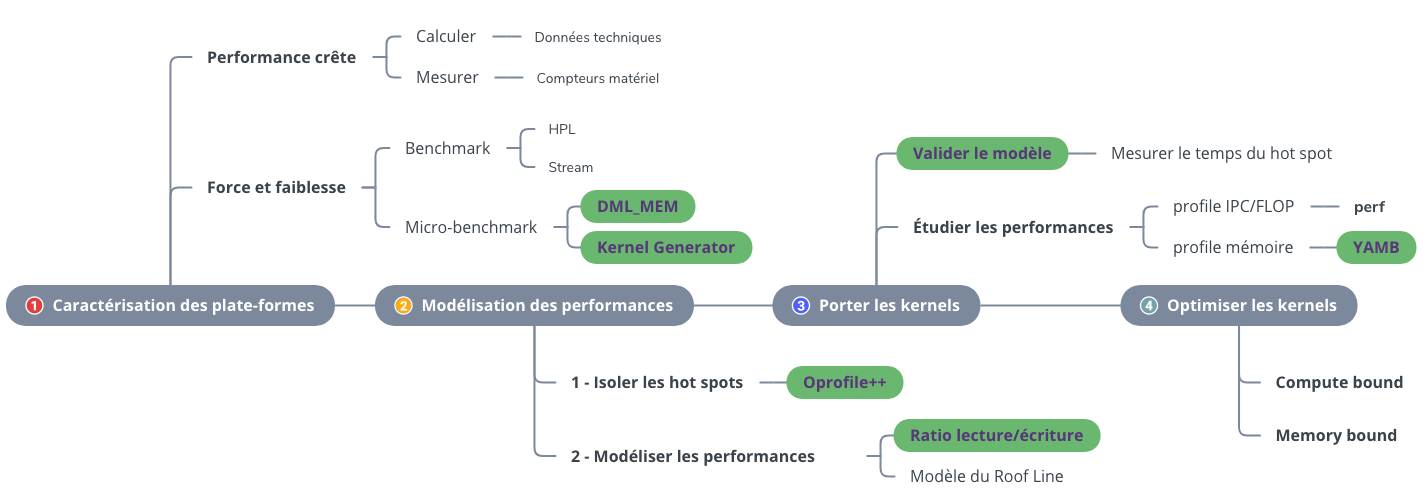
\includegraphics[width=\linewidth]{images/methodologie_step.png}
    \caption{\label{pic:methodologie_step_1} Méthodologie en 5 étapes pour caractériser et optimiser une application sur une nouvelle architecture. Les parties en vert représentent les développements présentés dans ce chapitre.}
    \end{figure}
    \textbf{TODO agrandir les caractère de cette image}
    
    Pour chaque étape, nous avons sélectionné les outils nécessaires pour répondre aux questions ce qui permet de poursuivre la méthodologie. Pour cela, nous avons réalisé un état de l'art des outils existants, sélectionné ceux répondant à nos critères de développement et développé les outils manquants.
    

        
\subsection{Critères de développement}
%%%%%%%%%%%%%%%%%%%%%%%%%%%%%%%%%%%%%%%%%%%%%%%%%%%%%%%%%%%%%%%%%%%%%%%%
    
    Pour sélectionner et développer les outils nécessaires à ce travail, nous avons établi une liste de critères à respecter:
    \begin{itemize}
        \item \textbf{La simplicité}: notre philosophie de développement repose sur l'utilisation d'outils simples répondant à une question précise. En développant des outils simples, le programmeur peut facilement en comprendre le déroulement et se l'approprier en apportant les modifications qu'il estime judicieuses. En proposant les outils en source ouverte, nous espérons que l'expérience des différents utilisateurs puisse profiter au reste de la communauté. Bien que certains travaux déplorent l'absence d'outils automatiques \cite{Chung2012}, nous estimons que la complexité des architectures et les multiples facteurs impactant la performance rendent impossible le développement d'outil automatique.\\
        
        \item \textbf{La compatibilité}: l'objectif de notre travail est la caractérisation de nouvelles plateformes, différentes de celles utilisées actuellement. Un critère majeur pour nos développements est d'assurer la compatibilité avec le maximum d'architectures. Le développement d'outils simples facilite d'autant plus la tâche du portage des outils. Ce critère interdit donc l'utilisation d'outils tels de \verb=VTune=, utilisable uniquement pour les architectures Intel.
        \textbf{TODO comme nous avons conclu dans la partie X que les compteurs matériels souffrent d'un ... même ceux d'un ...}Comme présenté dans la \autoref{sec:edl_hc_conclusion}, les compteurs matériels souffrent d'un manque de compatibilité entre les architectures (même d'un même constructeur) et peuvent être indisponibles sur des architectures de nouvelle génération. Les difficultés de programmation constaté dans l'état de l'art \textbf{todo c'est en annexe ça } nous ont contraint
        à ne sélectionner \textbf{todo check cette phrase} des outils se basant exclusivement sur des compteurs matériels standards. De plus, l'utilisation de compteurs plus complexes ne permet pas toujours de conclure facilement de la bonne ou mauvaise performance d'un code. Par exemple, un grand nombre de \textit{miss} dans le cache de niveau 1 n'implique pas forcément une mauvaise performance s'il s'agit d'un algorithme de \textit{stream}. Pour ces deux raisons, nous avons choisi d'utiliser et de développer des outils se basant uniquement sur des évènements simples: nombre de cycles, nombre d'instructions exécutées, instructions mémoire en cours et nombre de \textit{miss} \textbf{todo gls miss} dans le dernier niveau de cache.\\
        
        \item \textbf{La facilité d'utilisation}: le travail de caractérisation est une tâche très complexe. Si l'utilisation des outils doit être facilitée, il ne faut pas négliger la facilité d'installation. Plusieurs retours d'expérience nous ont montré que de nombreux utilisateurs n'utilisent pas certains outils lorsqu'ils ne parviennent pas à l'installer au premier essai. La réduction des dépendances à des librairies externes, et le développement d'outils simples nous assurent de réduire les difficultés lors de l'installation. De plus, dans des environnements industriels, l'utilisateur n'a pas toujours la liberté d'installer toutes les librairies qu'il souhaite le conduisant à renoncer à l'installation d'un outil. Les programmeurs qui travaillent quotidiennement sur des supercalculateurs savent que l'installation d'un outil, même simple, peut prendre du temps et de l'énergie : qu'il s'agisse de scripts de compilation complexes à déboguer ou de la dépendance vis-à-vis d’anciennes versions de bibliothèque. Pour ce faire, nos outils développés sont basés sur le nombre minimum de bibliothèques et l'outil de gestion de compilation libre de droits \textit{cmake}\footnote{CMake est un système de construction logicielle multiplateforme. Il permet de vérifier les prérequis nécessaires à la construction, de déterminer les dépendances entre les différents composants d'un projet (wikipédia) - \url{https://cmake.org/}}. CMake fait automatiquement la découverte et la configuration de la chaîne d'outils ce qui augmente la \textbf{portabilité} du code.
        Dans un environnement industriel, l'utilisateur n'aura pas non plus accès à des droits supplémentaires (\verb=root= ou \verb=kernel=). Nous avons donc sélectionné et développé des outils ne nécessitant pas ces droits. De plus, les compteurs matériels nécessitent des droits privilégiés, empêchant l'utilisation de nombreux outils existants. Cette raison est la principale motivation de l'utilisation du \textit{backend} de \verb=Perf Events= qui peut être rendu accessible à n'importe quel utilisateur. Bien que cette commande doive être exécutée par l'utilisateur \verb=root=, elle ne doit être exécutée qu'une seule fois à l'allumage de la machine:\\
        \verb|sudo sh -c 'echo 1 >/proc/sys/kernel/perf_event_paranoid'|\\
    
    \end{itemize}

        
        
\subsection{Organisation du chapitre}
%%%%%%%%%%%%%%%%%%%%%%%%%%%%%%%%%%%%%%%%%%%%%%%%%%%%%%%%%%%%%%%%%%%%%%%%
    
    Dans la \autoref{sec:edl_perf_intro} nous avons relevé le l'absence de plusieurs outils nécessaire pour accompagner l'utilisateur dans le travail de caractérisation d'architectures et d'analyse de performance d'applications. À notre connaissance ces outils n'existent pas. Soit ils EXISTENT PAS \textbf{TODO REPRENDRE} soit ceux existant ne répondent pas aux critères de développements n'ont soit pas pu être trouvés durant l'état de l'art du domaine, soit ils ne répondaient pas aux critères cités précédemment. Ce chapitre présente les 4 principaux outils développés lors de ce travail de thèse. Il suit la structure suivante:
   
   \begin{itemize}
       \item La \autoref{sec:dmlmem} présente un nouveau \gls{benchmark} permettant de réaliser des accès par sauts (strides) en mémoire pour des jeux de données de taille variable. Ce genre d'accès est très répandu dans les applications de type RTM \textbf{TODO expliquer RTM} et il est important de pouvoir caractériser la microarchitecture pour ces codes-là.
       \item La \autoref{sec:kg} introduit un générateur de benchmarks permettant de caractériser finement les unités de calcul arithmétique (ALU). Les architectures peuvent avoir des performances inégales et la performance de chaque instruction vectorielle doit être vérifiée pour valider la performance d'une application réelle (nombre d'instruction par cycle, fréquence supportée, opération flottante par seconde).
       \item La \autoref{sec:yamb} introduit un outil permettant de suivre l'évolution du trafic du bus mémoire. La mémoire étant une ressource critique des architectures modernes, cet outil est essentiel pour poursuivre la caractérisation des applications.
       \item La \autoref{sec:oprofile} présente un outil capable d'extraire le code assembleur des \gls{hotspot} d'une application et de caractériser chaque instruction ainsi que d'établir le résumé de la performance des boucles critiques.
   \end{itemize}
   
     


   
    %\subsubsection{Travaux existants}
    %%%%%%%%%%%%%%%%%%%%%%%%%%%%%%%%%%%%%%%%%%%%%%%%%%%%%%%%%%%%%%%%%%%%%%%%
    
        %\paragraph{Les outils de suivi de performance.} 
        
        %\paragraph{Les benchmarks.} Pour découvrir les caractéristiques d'une architecture, il est courant d'utiliser des programmes artificiels, appelés benchmarks, pour effectuer un certain type d'opération ou reproduire la même charge de travail qu'une application réelle. En HPC, deux benchmarks sont largement utilisés : le High Performance Linpack (HPL) \cite{Dongarra2003} mesure le taux d'exécution en virgule flottante pour résoudre un système d'équations linéaire. Le second, STREAM \cite{McCalpin1995}, est utilisé pour mesurer la bande passante mémoire durable pour un simple benchmark synthétique. Pour mieux représenter les applications réelles et avoir un classement des supercalculateurs, des suites de plusieurs benchmarks sont également utilisées telles que HPC Challenge \cite{Ang2016} ou HPCG \cite{dongarra2016high}. Pour caractériser plus précisément une partie de la microarchitecture, on peut utiliser d'autres codes tels que \textit{lmbench}. \cite{Staelin2004}. Il est composé de deux familles de benchmarks : une pour la bande passante mémoire et une pour la latence. Par exemple, il est capable de mesurer la latence de chaque niveau de cache de la mémoire. En raison de son incapacité à mesurer les performances du cache distant et les transactions de cohérence du cache, le benchmark \textit{x86-membench} benchmark \cite{Molka2017} a été développé pour supporter la mesure de la bande passante et de la latence du cache local ou distant, mais aussi de la mémoire. \newpage
        \section{Benchmark mémoire}\label{sec:dmlmem}

    La section suivante présente un benchmark mémoire appelé \textit{Demonstrate Memory Limit} ou \verb=DML_MEM=. Cet outil permet de vérifier le bon comportement de la hiérarchie mémoire lors d'accès mémoire à un jeu de donnée par sauts de taille constante. 

    

    \subsection{Motivations}
    %%%%%%%%%%%%%%%%%%%%%%%%%%%%%%%%%%%%%%%%%%%%%%%%%%%%%%
    
        L'industrie de la recherche pétrolière est un grand consommateur de calculs haute performance. Les applications utilisées utilisent des algorithmes de \textit{stencil}\footnote{En mathématiques, en particulier dans le domaine de l'analyse numérique, un stencil est un arrangement géométrique d'un réseau nodal qui se lie au point d'intérêt en utilisant une routine d'approximation numérique. Les stencils sont à la base de nombreux algorithmes de résolution numérique des équations aux dérivées partielles (EDP) (wikipédia).} qui impliquent des accès mémoire réguliers non contigus par \textit{sauts} aussi appelés \glspl{stride}. D'autres applications comme le calcul matriciel parcourent des matrices et génèrent des accès mémoire par saut de taille constante (multiple d'une taille d'une ligne). La \autoref{pic:dml_strides_acces_main} expose un exemple simple de tels accès. D'autres algorithmes peuvent réaliser ce genre d'accès par \textit{strides} comme les multiplications de matrices, les transformées de Fourrier ou le parcours d'un tableau de structures pour accéder à certains champs. Si les objets sont stockés continûment en mémoire, l'accès à un même champ de chaque objet réalise en réalité des accès mémoire par saut de taille fixes. 
        
        \begin{figure}[h!]
            \centering
                \begin{subfigure}[b]{0.25\linewidth}
                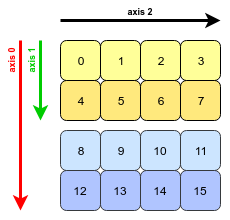
\includegraphics[width=\linewidth]{images/dml_strides_acces_matrix.png}
                \caption{Accès en ligne ou en colonne à une matrice.}
                \label{pic:dml_strides_acces_matrix}
                \end{subfigure}
            ~ %add desired spacing between images, e. g. ~, \quad, \qquad, \hfill etc. 
            %(or a blank line to force the subfigure onto a new line)
                \begin{subfigure}[b]{0.60\linewidth}
                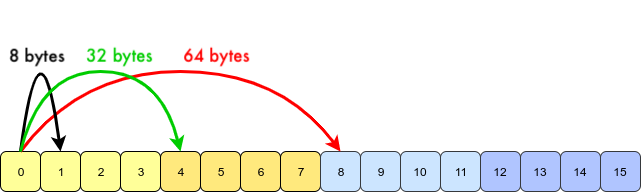
\includegraphics[width=\linewidth]{images/dml_strides_acces.png}
                \caption{Les accès en ligne ou en colonne impliquent des sauts en mémoire de différentes tailles.}
                \label{pic:dml_strides_acces}
                \end{subfigure}
            \caption{Exemple d'une application réalisant des accès en colonne à une matrice. Ces accès impliquent en réalité des sauts entre les adresses mémoires utilisées.}\label{pic:dml_strides_acces_main}
        \end{figure}
        % \subsubsection{Motivations}
    
    
        La grande majorité de ces applications ne réalisent pas suffisamment de calculs sur une donnée transférée pour masquer le temps de son accès mémoire. Ce déséquilibre de performance de l'architecture limite la performance de ces codes par celle du bus mémoire. 
        Pour ces applications, il est primordial que l'architecture soit capable d'anticiper le maximum des accès mémoire grâce à son matériel de prélecture mémoire (\textit{memory prefetcher}). Les \glspl{prelecteur} mémoires sont conçus pour anticiper les accès avant qu'ils ne soient réalisés pour réduire la latence d'accès. Lorsque les accès sont simples (taille régulière, proches en mémoire), la majorité des architectures modernes obtiennent de très bonnes performances. Cependant, les accès par sauts peuvent être grands (supérieurs à plusieurs lignes de cache) et lorsque de multiples accès sont réalisés en concurrence, le prélecteur peut rencontrer des difficultés à les anticiper. De plus, si le prélecteur mémoire anticipe de mauvais accès, le bus mémoire sera saturé de données inutiles au calcul. Le bus mémoire étant la ressource critique pour la majorité des applications HPC il est primordial que son utilisation soit la plus efficace possible.  
    
        

    \subsubsection{Objectifs}
        
        Le développement du benchmark \verb=DML_MEM= a été réalisé pour répondre à trois objectifs:
        \begin{enumerate}
            \item \textbf{Caractériser la performance} d'une architecture pour l'exécution d'applications utilisant un motif d'accès mémoire par strides. En mesurant ses performances, il est ensuite possible de prouver l’efficacité de l’utilisation du sous-système mémoire pour une application réelle utilisant ce type d'accès. En effet, nous montrons que pour vérifier la bonne performance d'une architecture pour une application donnée, il n'est pas suffisant de vérifier que le bus mémoire est saturé.
            \item \textbf{Attirer l'attention du programmeur} sur la complexité des architectures et de son impact sur les performances d'un code. Le benchmark développé doit pouvoir être utilisé pour caractériser l'ensemble de la hiérarchie mémoire: fonctionnement des caches et du prélecteur mémoire, saturation du bus mémoire, impact de l'utilisation de plusieurs coeurs... En appréhendant cette complexité, il sera plus simple pour le programmeur d'apporter les bonnes modifications à son code pour tirer la pleine performance du bus mémoire.
            \item \textbf{Aider à la conception} de nouvelles architectures en utilisant le benchmark pour vérifier le bon fonctionnement du système mémoire. En effet, en utilisant ce benchmark, nous avons trouvé certains dysfonctionnements majeurs dans un accélérateur prévu pour ce type d'applications. Grâce à notre outil, nous avons pu prouver que les performances théoriques de la plateforme n'étaient pas accessibles par l'application. 
        \end{enumerate}

    
    \subsubsection{Comparaison avec l'existant}
    %%%%%%%%%%%%%%%%
        L'étude des différents benchmarks existants est réalisée dans la \autoref{sec:edl_perf_intro}.  Au moment de la réalisation de ce travail de thèse, il n’existe à notre connaissance aucun benchmark permettant de caractériser l’architecture pour ce type d’accès. Le benchmark s’approchant le plus de cet objectif est celui de Saavedra \cite{Saavedra1995}. Il utilise une taille de saut fixée au début de l’exécution pour accéder à un jeu de données. Cependant, la taille de ce dernier doit être un multiple d’une puissance de 2 et ne permet pas de dépasser la taille du dernier niveau de cache. Comme le souligne \cite{Yotov2005}, le problème d’une telle approche est de vouloir mesurer tous les niveaux de la hiérarchie simultanément. Les mesures peuvent alors être influencées par différents paramètres de différents niveaux de caches. Ces mesures doivent être interprétées par l’utilisateur, le programme ne créant pas automatiquement la hiérarchie. Un second outil s'approchant de notre démarche est le benchmark DISBench \cite{disbench}. Cependant, il ne bénéficie d'aucune méthode solide de vérification de la performance comme celui implémenté par \verb=DML_MEM=. De plus, il n'est en aucun cas prévu pour faciliter le test de multiples tailles de strides sur différentes tailles de jeux de données. Le code n'est plus maintenu depuis 6 ans et ne peut pas être exécuté sans erreur lors de l'exécution.


\subsection{Le benchmark DML\_MEM}
%%%%%%%%%%%%%%%%%%%%%%%%%%%%%%%%%%%%%%%%%%%%%%%%%%%%%%
    Le motif d'accès par \gls{stride} est donc très courant dans le calcul haute performance. La distance entre deux accès peut varier d'une application, ou d'un jeu de données, à l'autre. Pour caractériser les plateformes pour ces applications, il est donc nécessaire de posséder un benchmark paramétrable permettant de faire varier la taille du jeu de données et la taille du saut. Cette section présente comment le benchmark \verb=DML_MEM= a été développé. Grâce à de nombreuses options nous montrons comment différentes parties de la microarchitecture peuvent être testée: caches, TLB, bus mémoire.


    \subsubsection{Concept}
    %%%%%%%%%%%%%%%%
        
        Le principe du benchmark est d'accéder à un tableau en utilisant différentes tailles de strides. Pour chaque stride une mesure de performance est réalisée. Une fois toutes les tailles de stride mesurée, le benchmark augmente la taille du jeu de données utilisé (voir \autoref{pic:dml_stride_intro}). La vitesse d'évolution de la taille des strides et du jeu de données peut être paramétrée. Les accès peuvent être réalisés en lecture ou en lecture/écriture.
       
        \begin{figure}[h!]
        \center
        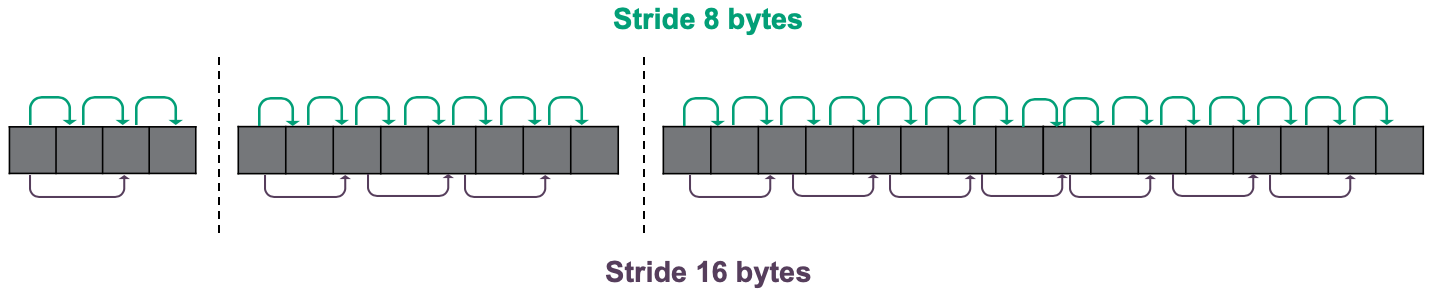
\includegraphics[width=14cm]{images/dml_stride_intro.png}
        \caption{\label{pic:dml_stride_intro}Évaluation de la performance de deux tailles de stride (8 et 16 bytes) sur trois jeux de données de tailles différentes.}
        \end{figure}


        Le benchmark se déroule en deux étapes: la configuration et son exécution.
        Lors de la configuration, les différents paramètres nécessaires pour l'exécution du benchmark sont extraits de la ligne de commande ou utilisent, le cas échéant, des valeurs par défaut. Les différentes versions du benchmark (mode d'accès, taille du déroulement des boucles) sont toutes compilées, l'initialisation utilise un pointeur de fonction vers la bonne version requise par l'utilisateur. Ensuite, le jeu de données est initialisé (voir \autoref{sec:dml_init}). 
        La deuxième étape consiste à exécuter le benchmark et à mesurer ses performances. Pour une taille de jeu de donnée et une taille de stride, la bande passante effective maximale, minimale ou moyenne est mesurée et affichée. Pour cela, le benchmark mesure le temps nécessaire pour réaliser le noyau de calcul. Celui-ci, renvoie le nombre d'accès réalisés grâce à l'initialisation du tableau durant la première étape. 
            \begin{verbatim}
time1 = get_micros();
num_ops = p->m_BENCHMARK();
time2 = get_micros();
bande_passante = calcul_bw(num_ops, time2 - time1);
            \end{verbatim}
            
        Ces mesures sont affichées au fur et à mesure de l'avancée du benchmark ainsi que dans un fichier de \textit{log}. Ce fichier peut ensuite être utilisé par un script pour afficher l'évolution de la performance de chaque stride en fonction de la taille du jeu de donnée. 
            
\begin{verbatim}
>./dml --type read --cacheline 64 --matrixsize 10000 --stride 8,64,256
...
Stride  S   ->          8         64        256
Value       ->    AVERAGE    AVERAGE    AVERAGE
       7.0 KiB     117.46          -          -
      81.0 KiB     114.29      88.24      74.12
      76.3 MiB      80.87      13.41       8.61
       7.5 GiB      80.35      13.11       7.18
...
\end{verbatim}

  

    \subsubsection{Les options}
    %%%%%%%%%%%%%%%%
        Le benchmark \verb=DML_MEM= accepte de nombreuses options. Grâce à celles-ci différentes configurations peuvent être utilisées pour tester différents scénarios sur différentes parties de la microarchitecture. Nous décrivons ici les options les plus utiles pour l'utilisateur. Les nombreuses options peuvent être affichées avec l'option \verb|--help|.
        
        
        \paragraph{-{}-stride, -{}-minstride, -{}-maxstride, -{}-stridemode} Ces quatre premières options permettent de définir quelles sont les différentes strides à utiliser pour réaliser les mesures. La première d'entre elles, permet à l'utilisateur de choisir une ou plusieurs à réaliser. Pour cela, une liste de taille de strides séparées par des virgules doit être entrée. Les trois dernières options permettent de générer automatiquement des strides à utiliser dans un intervalle $[min, max]$. L'option \verb|--stridemode| peut être utilisée avec les valeurs \textit{even} et \textit{odd} pour décaler les strides ainsi générées. Cela permet d'éviter des strides utilisant seulement des multiples de deux, pouvant être affectées par certaines caractéristiques de la microarchitecture (taille ligne de cache, taille des caches...). 
        
        \paragraph{-{}-matrixsize, -{}-minlog, -{}-maxlog, -{}-steplog, -{}-log} Ces 5 options permettent de définir la taille des jeux de données à utiliser. Leur taille évolue plus ou moins rapidement en fonction de la valeur de \verb|--steplog| jusqu'à atteindre la taille \verb|maxlog| ou bien celle de la matrice donnée avec l'option \verb|--matrixsize|. Si \verb|--steplog| est utilisé avec la valeur $0$, le benchmark réalise la mesure sur un seul jeu de données de la taille \verb=matrixsize=. L'option \verb|--log| permet de donner la même valeur à \verb|min| et \verb|max| pour ne réaliser la mesure que sur une taille de jeux de données. Couplée avec l'option \verb|--stride|, l'option \verb=--log= permet d'utiliser le benchmark pour n'accomplir qu'une seule mesure: un jeu de donnée, une stride.
        
        Ces 9 premières options sont les options principales du benchmark. Elles permettent de réaliser une multitude de mesures: performance des niveaux de caches, performance de la mémoire, fiabilité du \gls{prelecteur}, mesure de la taille d'une ligne de cache. Dans la \autoref{sec:dml_bad_stride} nous montrons comment ces options peuvent être utilisées pour identifier des tailles de strides ayant de mauvaises performances.
    
    
        \paragraph{-{}-type, -{}-unroll, -{}-mode} Ces trois options permettent de choisir le benchmark à utiliser. L'option \verb|--type| permet de réaliser les accès en lecture ou en lecture/écriture. La deuxième option permet d'appliquer l'optimisation du déroulement de boucle dont les différentes versions (déroulement de 2 à 64 fois) ont été programmées manuellement. La troisième option permet de choisir le mode d'accès. Par exemple l'utilisation de différents pointeurs pour réaliser plusieurs accès notamment lorsque l'option \verb|--unroll| est utilisée. L'analyse de la performance de ces options est réalisée dans la \autoref{sec:dml_unroll}.

        \paragraph{-{}-hugepages} Cette option permet d'allouer la mémoire pour le jeu de données en utilisant des pages de 2 MiB contre 4 KiB habituellement. La caractérisation des pages larges est réalisée dans la \autoref{sec:dml_large_page}.
        
        \paragraph{-{}-annotate} Cette option est utilisée lorsque l'activité du bus mémoire est mesurée avec l'outil YAMB présenté dans la \autoref{sec:yamb}. Le benchmark annote le graphique lorsqu'une nouvelle taille de stride ou de jeu de données est utilisée. Grâce à cette option, il est possible de corréler l'activité du bus avec une configuration particulière du benchmark. Cette option est utilisée dans la \autoref{sec:dml_cache_ok} pour mesurer l'activité du bus mémoire lorsqu'un jeu de donnée de la taille du dernier niveau de cache est utilisé. 

        \paragraph{Version parallèle} La dernière configuration du benchmark est la version parallèle utilisant MPI. Celle-ci doit être générée grâce à l'outil \textit{cmake} et la commande \verb|cmake -DOPT_BUILD_MPI=ON|. Grâce à cette version, plusieurs coeurs peuvent exécuter la même version du benchmark. Cette version du benchmark nous permet dans la \autoref{sec:dml_saturation} d'étudier l'évolution du débit mémoire lorsque des coeurs supplémentaires sont utilisés.
        
    
    \subsubsection{Validation des résultats} \label{sec:dml_init}
    %%%%%%%%%%%%%%%%

    Une grande difficulté lors de l'élaboration d'un benchmark a été de s'assurer que la performance mesurée était bien celle du code attendu. En effet, le compilateur peut appliquer certaines optimisations pour accélérer l'application. Ensuite, l'architecture elle-même peut se rendre compte de l'artificialité du code et en court-circuiter une partie. Dans les deux cas, le problème est que la mesure de la performance ne rend pas compte de la réalité du code et de la mesure attendue par le programmeur. 
    
    Pour éviter ces deux pièges, le benchmark \verb=DML_MEM= initialise le jeu de données avec deux valeurs suivant le type de l'accès voulu (lecture ou lecture/écriture). Lorsque le benchmark utilise des accès en lecture, le jeu de données est initialisé avec la valeur \textbf{1}, car chaque lecture occasionne un transfert sur le bus mémoire. 
    Lorsque le benchmark utilise le mode de lecture/écriture, le jeu de données est initialisé avec la valeur \textbf{2}. Chaque ligne doit être lue puis réécrite occasionnant deux passages sur le bus mémoire. Pour chaque accès la valeur contenue dans le tableau est stockée dans une variable de compteur.  L'utilisation de chaque valeur pour l'ajouter au compteur empêche le compilateur et l'architecture d'appliquer certaines optimisations. À la fin de l'exécution, le benchmark retourne cette variable permettant de compter le nombre total d'accès \textbf{effectivement} réalisés.
    

    
    
    
    
    
    
    
    
\subsection{Expérimentations et principaux résultats}
%%%%%%%%%%%%%%%%%%%%%%%%%%%%%%%%%%%%%%%%%%%%%%%%%%%%%%

    Dans cette section nous présentons les principaux résultats obtenus avec le benchmark \verb=DML_MEM=. L'objectif est de montrer au lecteur les différentes mesures rendues possibles par l'utilisation de l'outil. Les tests sont principalement réalisés sur l'architecture des processeurs Intel Skylake. 


    \subsubsection{Impact du choix du compilateur sur la performance}
    %%%%%%%%%%%%%%%%
    
        Contrairement au benchmark du générateur de kernel (voir \autoref{sec:kg}), le code de \verb=DML_MEM= n'est pas écrit directement en assembleur. La qualité du compilateur peut donc avoir un impact significatif sur ses performances. Avant de réaliser plus d'expérimentations, nous avons testé deux compilateurs (GCC 8.2 et ICC 19.0) avec différents drapeaux de compilation. Avec d'anciennes versions de GCC (telle que la version 4.8), nous avons mesuré une amélioration d'un facteur deux en utilisant les drapeaux \verb|-O3 -march=skylake-avx512|. Le compilateur ayant reçu de nombreuses améliorations depuis, nous n'avons trouvé aucun drapeau permettant d'améliorer les performances de ce dernier. Nous l'avons comparé avec la version 19.0 du compilateur d'Intel ICC couplé avec le drapeau \verb|-O3|. Les performances mesurées dans les différents niveaux de la hiérarchie mémoire sont présentées dans le \autoref{tab:dml_compiler}.

        \begin{table}[h!]
        \centering
        \begin{tabular}{|l|c|c|}
        \hline
        Niveau de la hiérarchie & GCC 8.2 & ICC 19.0 \\ \hline
        L1 & 58 & 310 \\ \hline
        L2 & 56 & 161 \\ \hline
        L3 & 26 & 26 \\ \hline
        Memory & 12.5 & 12.5 \\ \hline
        \end{tabular}%
        \caption{Performance du benchmark \texttt{DML\_MEM} configuré pour mesurer le débit maximal (GB/s) atteignable pour quatre niveaux de la hiérarchie mémoire. Le benchmark compare la performance atteignable lors de l'utilisation des compilateurs GCC et ICC. Le drapeau d'optimisation \text{-O3} est utilisé dans les deux cas.}
        \label{tab:dml_compiler}
        \end{table}

        Lorsque le jeu de données tient dans le premier niveau de cache, nous avons mesuré des différences de performances du benchmark pouvant aller jusqu'à un facteur 8. Cet écart de performance entre les deux compilateurs se réduit lorsque la taille du jeu de données augmente. En effet, nous mesurons des performances équivalentes pour les deux versions de compilateurs lorsque le jeu de donnée accédé est localisé en mémoire. Nous expliquons l'écart de performance constaté dans les premiers niveaux de cache par la mauvaise performance du code généré par le compilateur GCC. Le premier niveau de cache des processeurs Skylake est capable de fournir 128 octets par cycle, soit une bande passante de 345 GB/s. Le code généré par GCC ne parvient pas à utiliser plus de 58 GB/s. Nous avons mesuré que le benchmark compilé par GCC utilisé deux fois plus d'instructions que celui compilé par ICC. La performance du benchmark compilé par GCC n'est alors pas limitée par la performance du bus mémoire (\gls{memorybound}) mais par celle du processeur (\gls{computebound}). La bande passante disponible se réduisant lorsqu'on \textit{remonte} les niveaux de la hiérarchie mémoire, l'impact de la qualité du code est aussi réduit. Les performances du benchmark compilé par ICC étant toujours supérieures à celles produites par GCC, nous utiliserons le compilateur d'Intel dans les prochaines expérimentations. Lorsque de nouvelles versions sont disponibles ou que d'autres architectures sont étudiées, nous conseillons de toujours tester les différentes versions de compilateurs avec les drapeaux de compilation adéquats. Ce constat réalisé sur notre benchmark et aussi applicable pour une application réelle.
    
    
    \subsubsection{Mesurer la taille d'une ligne de cache}
    %%%%%%%%%%%%%%%%
    
        Les transferts de données entre la mémoire et le processeur sont réalisés par paquet de données appelés \textit{ligne de cache}. L'origine et les propriétés des caches sont présentées dans l'\aref{sec:cache}. Connaître la taille d'une ligne de cache de l'architecture est nécessaire pour obtenir les mesures correctes par le benchmark. Cette taille peut aussi être nécessaire lors du développement d'une application pour disposer les données de façon optimale. Nous montrons dans cette expérimentation comme celle-ci peut être retrouvée en utilisant le benchmark \verb=DML_MEM=. Pour cela, nous désactivons le \gls{prelecteur} mémoire (memory prefetcher) pour l'empêcher d'anticiper le chargement d'une ou plusieurs lignes de cache avant son accès. Le jeu de données utilisé doit quant à lui être plus grand que le dernier niveau de cache. La taille des lignes de cache des architectures modernes est généralement comprise entre 32 et 256 bytes. Nous utilisons le benchmark pour mesurer la performance du système mémoire en utilisant des \glspl{stride} de puissance de 2 allant de 8 à 256 bytes. Les performances ainsi mesurées sont présentées dans le \autoref{tab:dml_cache_line}.
    
        \begin{table}[h!]
        \centering
        \begin{tabular}{|l|c|c|c|c|c|c|}
        \hline
        Taille de la stride (byte) & 8 & 16 & 32 & 64 & 128 & 256 \\ \hline
        Bande passante (GB/s) & 31.58 & 25.84 & 14.50 & 7.62 & 7.65 & 7.62 \\ \hline
        \end{tabular}%
        \caption{Pour un jeu de données de 1 GiB, mesure de la performance de plusieurs tailles de stride lorsque le prélecteur mémoire est désactivé.}
        \label{tab:dml_cache_line}
        \end{table}
        
         L'interprétation de ces résultats doit être la suivante. Pour des \glspl{stride} de 64, 128 ou 256 bytes, la performance est la même. Il est important de rappeler que le benchmark mesure le débit mémoire atteint par l'application et non le trafic mémoire du bus. La performance de ces trois strides est égale.  Peut importe la taille du saut réalisé, la donnée accédée lors du prochain accès sera sur une autre ligne de cache. Ceci indique que pour ces trois cas, le processeur attend une ligne de cache pour réaliser un accès.  Lorsqu'une stride de 32 bytes est utilisée, la performance double, indiquant que la taille d'une ligne de cache est de 64 bytes. En effet, le processeur est capable de réaliser deux fois plus d'accès. Ceci est possible, car lorsqu'un premier accès est réalisé sur une ligne de cache, le suivant le sera aussi. La donnée est alors déjà présente dans le cache L1. L'utilisation d'une stride de 16 bytes améliore encore la performance du benchmark sans doubler pour autant. En effet, comme dans la première expérimentation le code devient \gls{computebound}. Le benchmark additionne des nombres flottants et la performance du code est alors limitée par l'ALU. 
    
    
    \subsubsection{Performances de différentes tailles de strides} \label{sec:dml_bad_stride}
    %%%%%%%%%%%%%%%%
        
        Un objectif principal de notre benchmark est de vérifier le bon comportement du processeur lors d'accès mémoire utilisant des sauts d'adresse de taille constante. Pour cela, nous avons développé un script qui permet d'exécuter le benchmark avec un grand nombre de strides et d'afficher leur performance dans un graphique. La \autoref{pic:dml_strides_bad} montre le résultat d'une telle exécution. Pour chaque \glspl{stride} et chaque taille de jeu de données, une mesure est réalisée. Pour faciliter la lecture du graphique, nous avons coloré les strides en fonction de leur taille en allant du bleu (pour les strides les plus petites) au rouge (pour les plus grandes). Nous remarquons que les strides de grande taille (plusieurs MiB) ont de meilleures performances que celle de petite taille. En effet, même pour des tailles de jeu de données de plusieurs centaines de mégaoctets (ne pouvant pas tenir dans le cache), le benchmark mesure des performances similaires à si le jeu de données se trouvait dans le cache. En réalité, pour des grandes tailles de strides, le jeu de données réellement utilisé par le benchmark peut être contenu dans les différents niveaux de cache. 
      
        \begin{figure}
        \center
        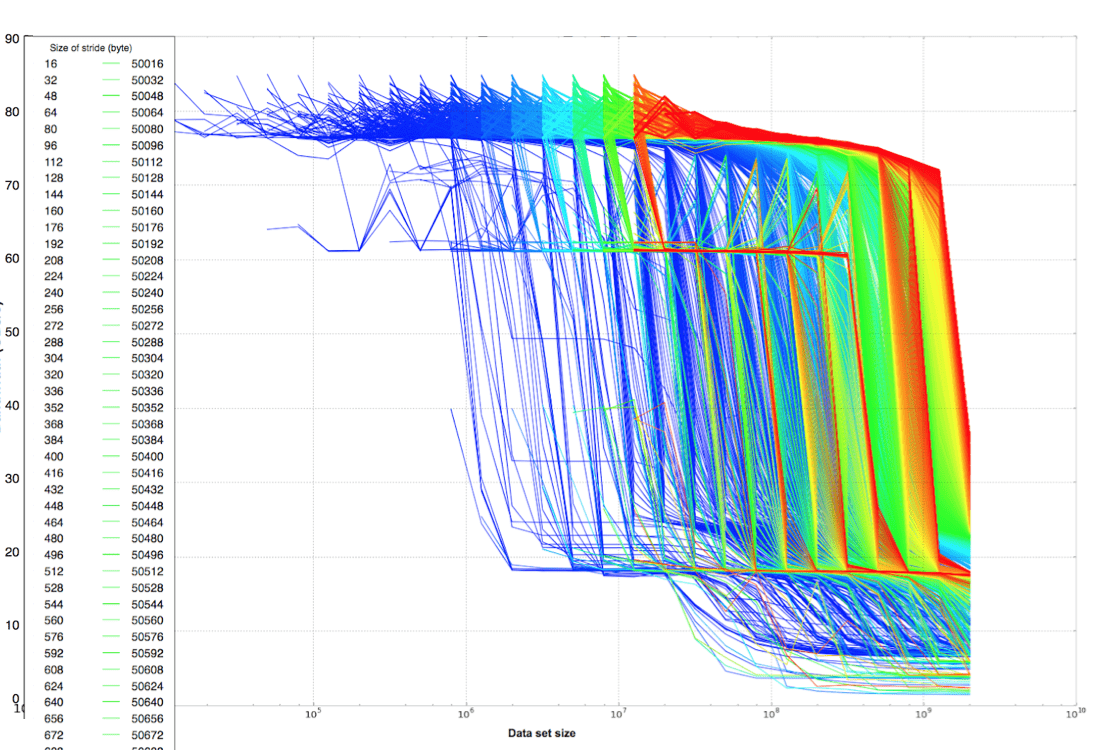
\includegraphics[width=12cm]{images/dml_strides_bad.png}
        \caption{\label{pic:dml_strides_bad} Performance du benchmark donnée en GB/s pour différentes tailles de strides représentées par des couleurs allant du bleu (petite taille) au rouge (grande taille). Nous remarquons que certaines strides de taille similaire ont des performances très inégales.}
        \end{figure}
        
        Nous remarquons sur la \autoref{pic:dml_strides_bad} que certaines \glspl{stride} ont des comportements différents que des strides de tailles proches (donc de couleurs proches aussi). En effet, des groupes de strides ont des performances bien plus faibles que d'autres et les mêmes résultats sont obtenus en utilisant des pages larges pour réduire l'impact sur la TLB. Nous avons isolé certaines d'entre elles et reporté leur performance dans le  \autoref{tab:dml_bad_strides}. Pour réaliser ces mesures, la commande suivante a été utilisée: 
        \begin{verbatim}
./dml --steplog 0.01 --unroll 8 --mode special --type read --cacheline 64 
      --stride 73704,73728,77816,77824,81928,81920 --measure 10 --matrixsize 10000
        \end{verbatim}
        
        
        \begin{table}[h!]
        \centering
        \begin{tabular}{|c|c|c|c|c|}
        \hline
        \rowcolor[HTML]{EFEFEF} 
        Taille de la stride (byte) & Débit mémoire mesuré (GB/s) & Nb. inst. & IPC & LLC Miss \\ \hline
        \rowcolor[HTML]{FFFFC7} 
        73704 & 24.54 & 690071400 & 0.34 & 21100474 \\ \hline
        \rowcolor[HTML]{FFFFC7} 
        73728 & 2.04 & 690064918 & 0.22 & 30612018 \\ \hline
        \rowcolor[HTML]{E8FFFE} 
        77816 & 24.53 & 688909428 & 0.33 & 21152403 \\ \hline
        \rowcolor[HTML]{E8FFFE} 
        77824 & 4.01 & 688905576 & 0.27 & 30144907 \\ \hline
        \rowcolor[HTML]{E6FFE6} 
        81928 & 24.76 & 690692156 & 0.33 & 21194483 \\ \hline
        \rowcolor[HTML]{E6FFE6} 
        81920 & 4.03 & 690693382 & 0.27 & 30794354 \\ \hline
        \end{tabular}%
        \caption{Mesure du débit mémoire atteint, du nombre d'instructions exécuté et le débit de leur exécution (Instruction Par Cycle) ainsi que le nombre de \textit{miss} mesuré dans le dernier niveau de cache (LLC) pour trois couples de strides de taille similaire.}
        \label{tab:dml_bad_strides}
        \end{table}
        
        
        Le benchmark qui utilise une \textit{mauvaise} stride (73728, 77824 ou 81920) voit sa performance limitée par la latence du système mémoire  (\textit{latency bound}). En effet, nous avons réalisé différentes mesures telles que le nombre de \textit{miss} du dernier niveau de cache ou l'activité du bus mémoire. L'analyse de l'activité du bus mémoire montre qu'il est loin d'être saturé. Si la ligne de cache n'est pas présente dans un des niveaux de cache, et que le bus n'est pas saturé, c'est que le processeur l'attend et n'a pas anticipé son manque (\textit{miss}). On remarque que l'IPC est plus faible et que le nombre de \textit{miss} est lui plus élevé pour ces strides. La question est alors de savoir pourquoi pour une certaine taille la ligne de cache est présente dans le cache et que pour une stride plus grande de quelques bytes elle n'y soit pas. L'explication vient de la taille des strides utilisées. Nous avons utilisé des strides de taille $ Stride_{n+1} = Stride_n + 16 ~ bytes$ avec $Stride_0 = 16 ~ bytes$. En utilisant des tailles de multiple de 16, certaines d'entre elles génèrent des conflits avec la politique de remplacement de lignes de caches. Ainsi, ces tailles de saut particulières mettent la pression seulement sur une partie du cache, le rendant inefficace. Le processeur doit donc attendre pour une majorité des accès, que la ligne de cache soit transférée depuis la mémoire. La performance du code est alors limitée par la latence du système mémoire (\textit{latency bound}).
        
        Nous avons ensuite réalisé la même expérimentation en décalant la taille des strides utilisées en commençant avec une stride minimale $Stride_0 =  8 ~ bytes$. Ainsi, aucune stride utilisée n'est multiple de 32, et aucune d'entre elles n’obtient de performance inattendue (voir \autoref{pic:dml_strides_good}).
        
        
        \begin{figure}
        \center
        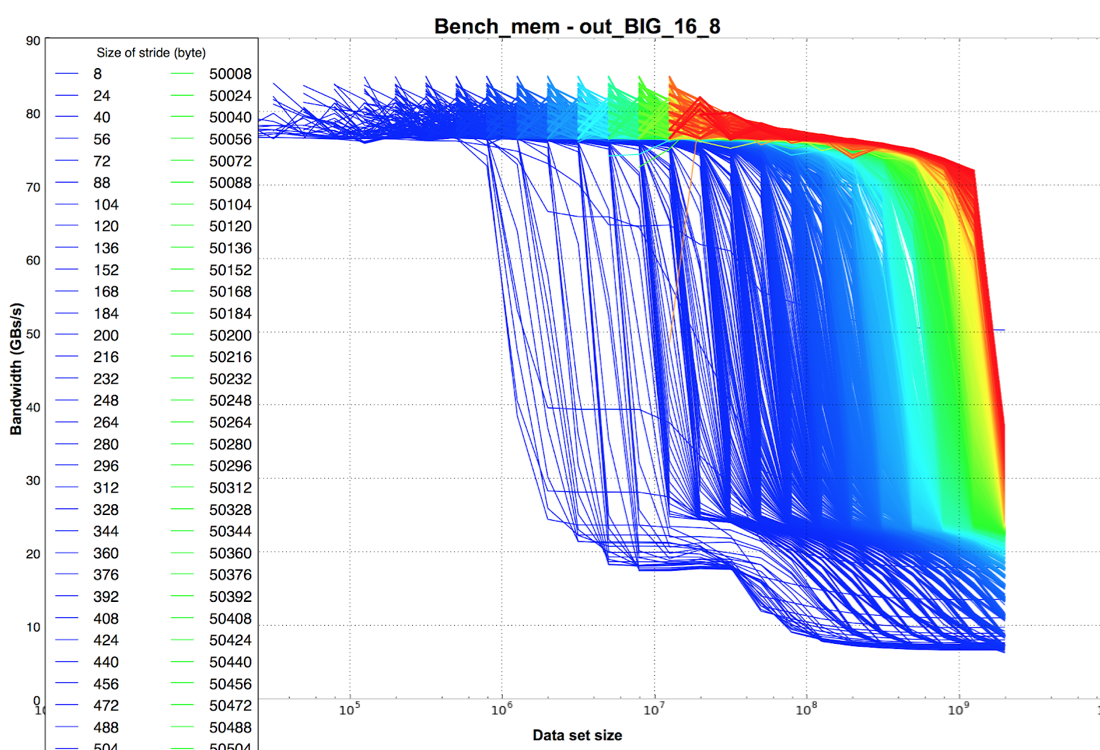
\includegraphics[width=12cm]{images/dml_strides.png}
        \caption{\label{pic:dml_strides_good} Performance du benchmark pour différentes tailles de strides (couleurs).  }
        \end{figure}
        
        À travers cette expérimentation, nous avons voulu montrer qu'un code aussi simple qu'il est peut avoir des performances inattendues. La complexité des architectures modernes est telle qu'elle peut avoir une incidence forte sur la performance des applications. Pour des strides aussi longues (plusieurs MiB), le \gls{prelecteur} mémoire ne semble pas arriver à anticiper ces accès. Si une application réalise ce type d'accès, le programmeur doit s'assurer de ne pas réaliser des strides de cette taille en ajoutant du \textit{padding} (remplissage) pour décaler artificiellement les données accédées. Une autre optimisation lors d'accès à certains champs d'objets contenus dans un tableau est de regrouper ces mêmes champs dans une structure spécifique. Ainsi, ces champs sont contigus en mémoire. 
        

    \subsubsection{Saturation du bus mémoire}\label{sec:dml_saturation}
    %%%%%%%%%%%%%%%%
        Pour pouvoir modéliser la performance des applications (modèle du \textit{Roof Line}) il est courant d'utiliser les performances maximales atteignables par une ressource. Pour cela, nous avons exécuté le benchmark en utilisant différents nombres de coeurs. Les résultats sont visibles sur le graphique de la \autoref{pic:dml_bw_mpi}. Sur ce processeur, notre benchmark arrive à obtenir une bande passante mémoire maximale de 114 GB/s. À titre de comparaison, le benchmark STREAM permet d'atteindre un débit mémoire de 108 GB/s. La loi de Little ne permet pas à un seul coeur de saturer la totalité du bus mémoire. Nous montrons à travers cette expérimentation qu'il faut au moins 15 coeurs pour le saturer. Les coeurs supplémentaires ne permettent pas ensuite d'améliorer le débit mémoire, car le bus est saturé. Pour des codes \gls{memorybound}, il peut alors être intéressant d'en désactiver certains ou de ne pas investir dans des processeurs avec plus de coeurs. Nous présentons dans la \autoref{sec:dml_core_vs_freq} un script permettant de réaliser cette recherche du nombre minimal de coeurs permettant de saturer le bus mémoire. 
        
        \begin{figure}
        \center
        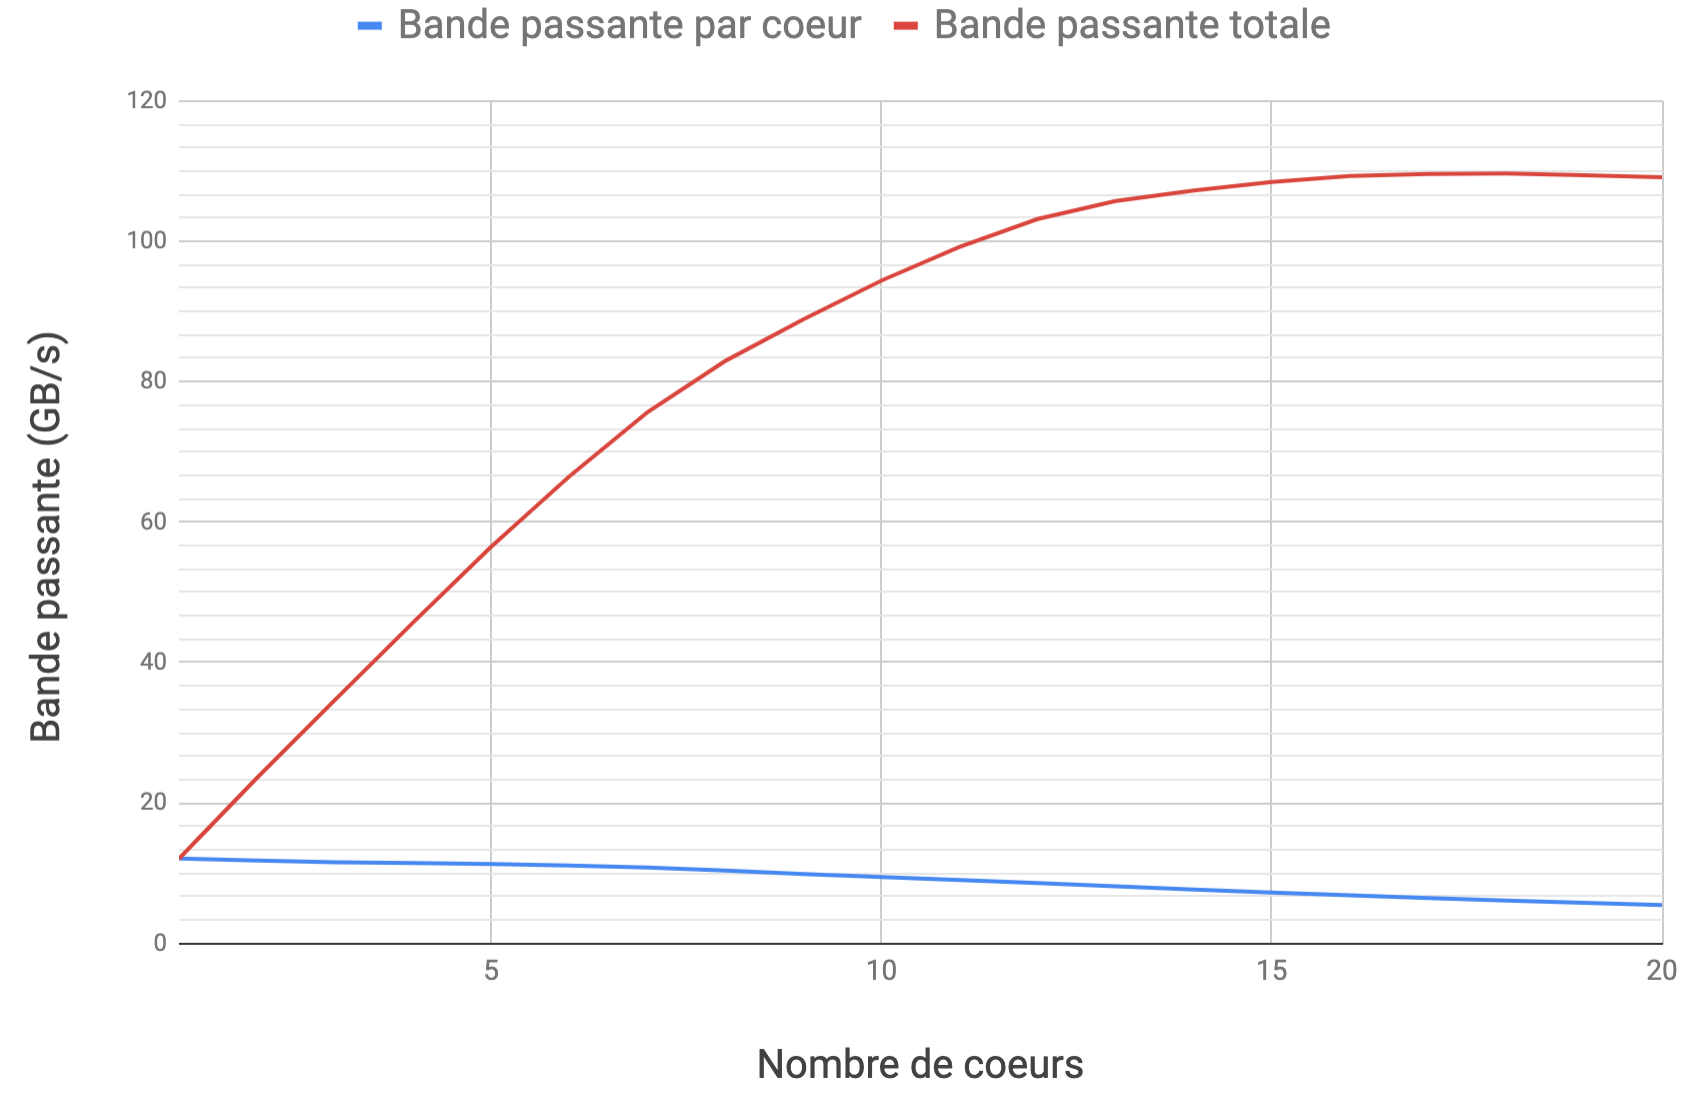
\includegraphics[width=10cm]{images/dml_bw_mpi.png}
        \caption{\label{pic:dml_bw_mpi} Bande passante mémoire atteinte pour différent nombre de coeurs}
        \end{figure}
        
    
    
    

    \subsubsection{Vérifier le bon fonctionnement des caches} \label{sec:dml_cache_ok}
    %%%%%%%%%%%%%%%%
        Les caches des architectures modernes se sont complexifiées et sont devenues très efficaces pour accélérer les accès mémoires. Cependant, sur des architectures différentes que celles utilisées communément, il peut être intéressant de vérifier leur bon fonctionnement. Nous montrons dans cette expérimentation les tests pouvant être réalisés.
        
        La première vérification est de s'assurer de l'indépendant des caches propres à chaque coeur. Dans le cas des processeurs Skylake, les deux premiers niveaux sont privés à chaque coeur. Nous avons implémenté une option pour annoter la taille de niveau de cache sur le graphique final. Les résultats de deux exécutions sur 1 et 20 coeurs sont présentés sur la \autoref{pic:dml_cache}. Comme attendu, la performance du benchmark n'est pas impactée lorsque le jeu de données utilisé est situé dans les caches L1 et L2. Les performances se dégradent lorsque le jeu de données commence à remplir le dernier niveau de cache, commun à tous les coeurs.
        
        \begin{figure}
        \centering
            \begin{subfigure}[b]{0.47\linewidth}
            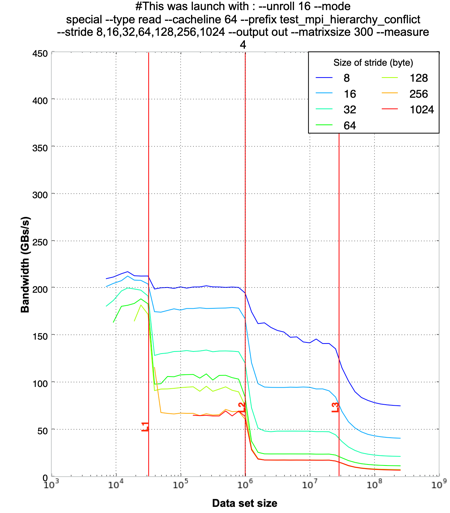
\includegraphics[width=\linewidth]{images/dml_cache_1core.png}
            \caption{Performance mesurée lors de l'utilisation d'un seul coeur}
            \label{pic:dml_cache_1core}
            \end{subfigure}
        ~ %add desired spacing between images, e. g. ~, \quad, \qquad, \hfill etc. 
        %(or a blank line to force the subfigure onto a new line)
            \begin{subfigure}[b]{0.47\linewidth}
            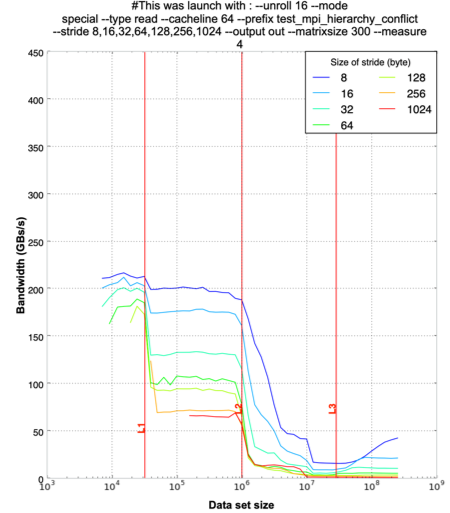
\includegraphics[width=\linewidth]{images/dml_cache_20core.png}
            \caption{Performance mesurée lorsque les vingt coeurs du processeur sont utilisés}
            \label{pic:dml_cache_20core}
            \end{subfigure}
        \caption{Performance du système mémoire mesurée à l'aide du benchmark \texttt{DML\_MEM} lors de sont exécution par 1 coeur (a) et vingt coeurs (b). Les résultats montrent que les caches L1 et L2 ne sont pas affectés par l'utilisation d'autres coeurs. Le débit mémoire disponible par coeur s'effondre lorsque plusieurs coeurs utilisent un jeu de données situé dans le cache L3.}\label{pic:dml_cache}
        \end{figure}
        
        Une deuxième expérimentation pouvant être menée au niveau des caches est la vérification du fonctionnement du cache L3. Pour cela, nous utilisons un jeu de donnée dont la taille évolue jusqu'à remplir le cache L3.  En parallèle, nous mesurons l'activité sur le bus mémoire avec l'outil YAMB, présenté dans la \autoref{sec:yamb}. Les résultats de cette expérimentation sont montrés sur la \autoref{pic:dml_L3_sharing} et peut être réalisée avec les commandes suivantes:
        \begin{verbatim}
./monitoring_bw_main.sh --start
./dml --steplog 0.01 --unroll 2 --type read --cacheline 64 --stride 64  
      --matrixsize 100 --measure 1000 --minlog 6.1 --annotate log_mem.annotate
./monitoring_bw_main.sh --stop
        \end{verbatim}
        
         \begin{figure}
        \center
        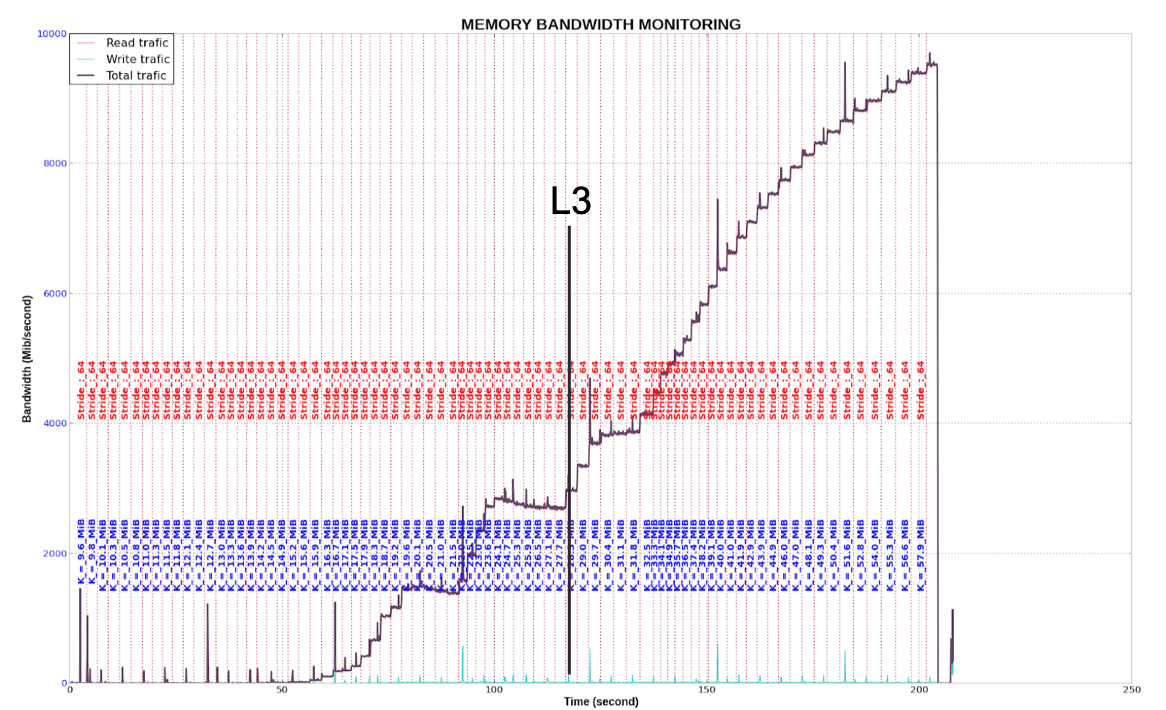
\includegraphics[width=14cm]{images/dml_L3_sharing.png}
        \caption{\label{pic:dml_L3_sharing} Évolution de l'activité du bus mémoire en fonction de la taille du jeu de donnée.}
        \end{figure}
        
        Nous montrons ainsi que pour un cache L3 de 28 MiB ne parvient pas à garder la totalité d'un jeu de donnée dépassant les 16 MiB. Au-delà de cette taille, YAMB mesure de l'activité sur le bus mémoire pouvant atteindre les 3 GB/s pour un jeu de donnée de la taille du L3 (28 MiB). Cette mauvaise utilisation du cache peut être due au phénomène de coloration de page discuté dans les expérimentations suivantes. Cette caractéristique impacte la performance de chaque coeur, car certaines données sont éjectées du cache et génèrent un évènement de \textit{miss}. Nous avons réalisé une seconde expérimentation en utilisant deux jeux de données de 20 et 28 Mib. Pour chaque jeu, nous utilisons progressivement la totalité des coeurs. Le résultat présenté sur la \autoref{pic:dml_bw_cacheL3} montre que le phénomène de \textit{trash} est encore plus fort lorsque plusieurs coeurs sont utilisés. Le trafic généré atteint les 19 GB/s pour 6 coeurs se partageant un jeu de données de 28 MiB. Cependant, la performance entre les deux benchmarks est identique, permettant de conclure du bon fonctionnement du prélecteur mémoire. Si une architecture ne possède pas un composant aussi efficace, il peut alors être intéressant de réduire la taille des jeux de données utilisés. Pour certaines optimisations comme le \textit{cache blocking}, nos expérimentations nous ont montré que d’utiliser 80\% de la capacité du dernier niveau de cache était le plus efficace.
        
        \begin{figure}
        \center
        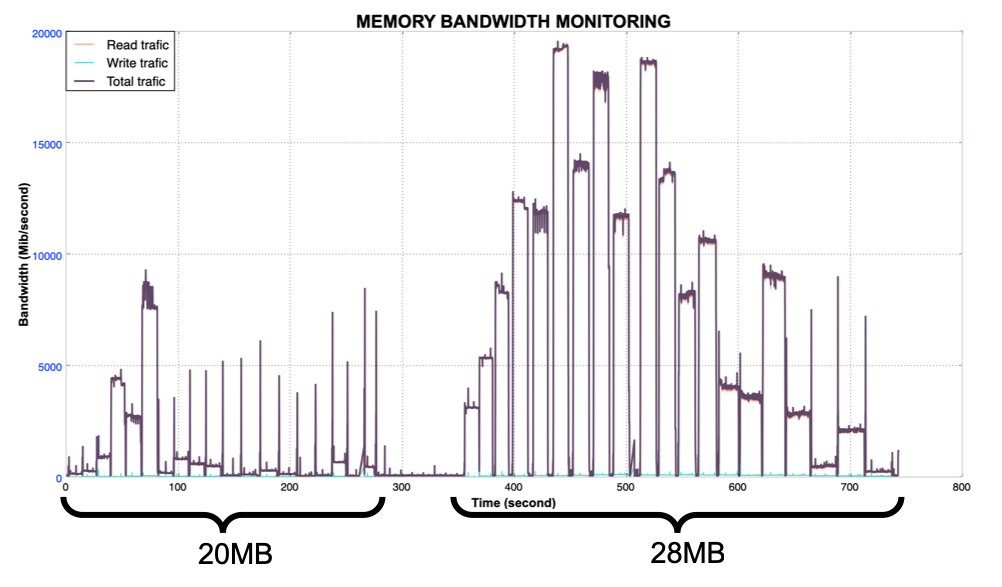
\includegraphics[width=14cm]{images/dml_bw_cacheL3.png}
        \caption{\label{pic:dml_bw_cacheL3} Évolution du trafic mémoire pour deux jeux de données de 20 et 28 MiB. Chaque jeu est accédé par 1 à 20 coeurs.}
        \end{figure}
        
        

    \subsubsection{Prélecteur mémoire}
    %%%%%%%%%%%%%%%%
        
        Dans l'expérimentation précédente, nous avons vu que le \gls{prelecteur} permettait de maintenir la bonne performance du benchmark même lorsque des données sont évincées du cache. Dans cette partie nous questionnons l'utilité de son activation permanente à l'aide de trois expérimentations:
        \begin{enumerate}
            \item Débit mémoire atteignable par différent nombre de coeurs lors de l'activation ou non du prélecteur.
            \item Débit mémoire atteignable par un coeur lorsque le prélecteur est activé ou non pour différentes tailles de \glspl{stride}.
            \item Débit mémoire atteignable par différent nombre de coeurs lorsque le prélecteur est activé ou non pour une taille de \textit{stride} correspondant à la taille de deux lignes de cache.
        \end{enumerate}

        
       \paragraph{Impact de l'activation ou non du prélecteur.} 
            Si une architecture possède un prélecteur mémoire défaillant, il peut être intéressant de vérifier si les coeurs du processeur sont capables de générer suffisamment de requêtes mémoires pour saturer le bus.
            En utilisant la version parallèle de \verb=DML_MEM=, nous avons mesuré la performance du benchmark lorsque le mécanisme de prélecture était actif ou non, avec différent nombre de coeurs. Le benchmark a été configuré pour utiliser des sauts de 64 bytes (une ligne de cache). Ce type d'accès correspond à un algorithme de \textit{stream} accédant à toutes les données.  La \autoref{pic:dml_prefetch_mpi} montre que si le prélecteur est désactivé la totalité des coeurs ne suffisent pas à saturer le bus mémoire. Dans ce cas-là, il peut alors être intéressant de réaliser le préchargement manuellement.
        
                \begin{figure}
                \center
                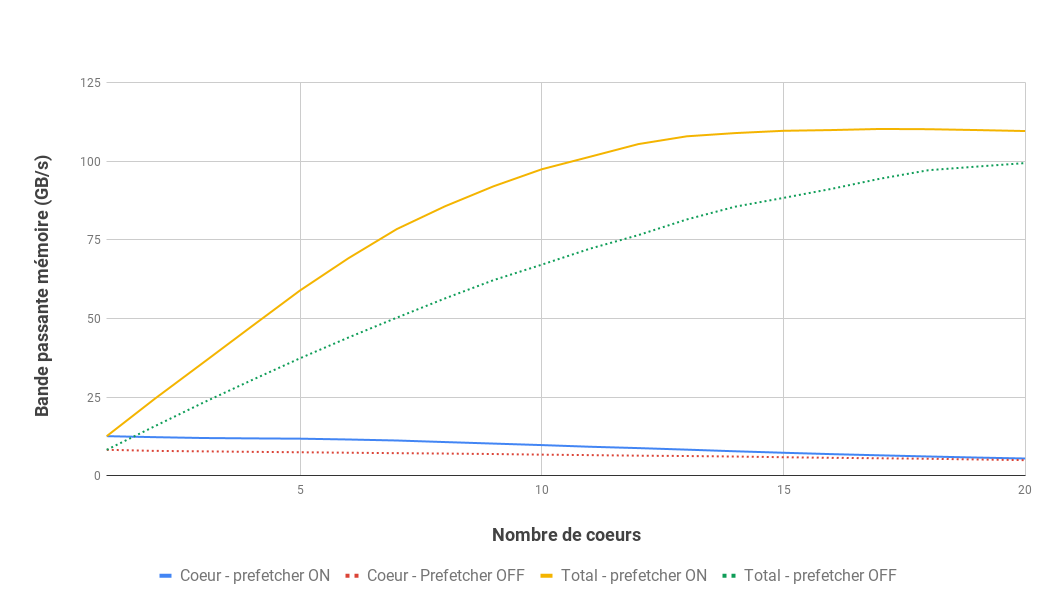
\includegraphics[width=14cm]{images/dml_prefetch_mpi.png}
                \caption{\label{pic:dml_prefetch_mpi} Performance du benchmark pour un jeu de données de 300 MiB avec un et plusieurs coeurs actifs lorsque le prélecteur adjacent activé ou non. La stride utilisée est égale à la taille d'une ligne de cache (64 bytes).}
                \end{figure}

        
        \paragraph{Utilisation d'un coeur.}
            Si le prélecteur est efficace pour l'exécution d'un algorithme de \textit{stream}, il est important de vérifier son bon fonctionnement pour d'autres types d'accès. Ainsi, nous avons exécuté le benchmark \verb=DML_MEM= pour utiliser différentes tailles de \textit{strides} lors de l'accès au jeu de données lorsque le prélecteur était actif ou non. La \autoref{pic:dml_prefetch} montre débit mémoire atteint par un seul coeur  pour des sauts allant de 64 à 3700 bytes. On remarque que les performances sont similaires sauf pour une \textit{stride} de 64 bytes, correspondant à la taille d'une ligne de cache. Pour une telle taille de \textit{stride}, la bande passante mémoire atteinte est réduite de 40\% lorsque le prélecteur est désactivé. La raison de cette baisse vient d'un mécanisme couramment utilisé dans les architectures appelé le prélecteur adjacent (\textit{adjacent prefetch}. Les codes parcourent souvent la mémoire de façon contiguë (données d'un tableau, instruction d'un programme). Ainsi, lors d'un accès mémoire, le prélecteur adjacent anticipe les futurs accès en chargeant aussi la ligne de cache suivante. Avec l'utilisation d'une \textit{stride} de 128 bytes, nous remarquons que le mécanisme de prélecture n'améliore plus les performances, car il ne s'occupe de charger que la ligne de caches adjacente. Lorsque celui-ci est activé, le bus mémoire transfère alors des données inutilisées pouvant affecter la performance d'une application.
            
            
        
        \begin{figure}
        \center
        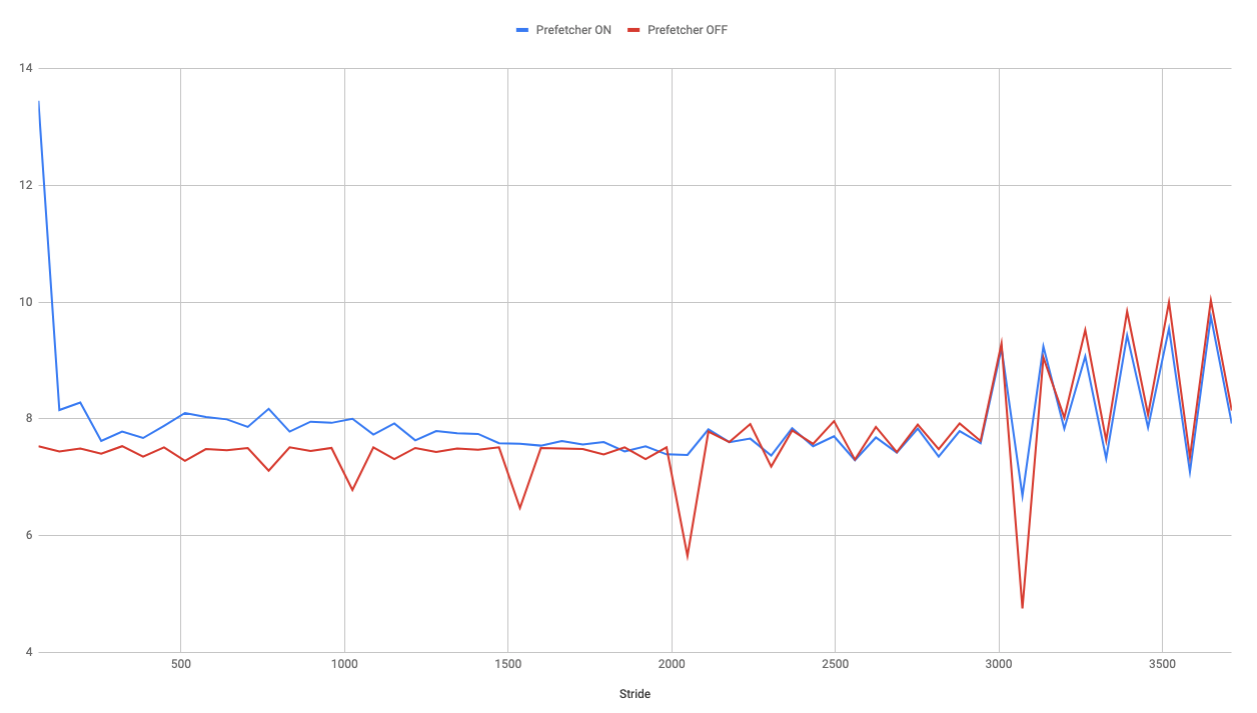
\includegraphics[width=10cm]{images/dml_prefetch.png}
        \caption{\label{pic:dml_prefetch} Débit mémoire atteint par un coeur (en GB/s) lors de l'activation (en bleu) ou non (en rouge) du prélecteur mémoire pour différentes tailles de stride. }
        \end{figure}
        
        
        
         
        \paragraph{Utilisation de tous les coeurs.} 
            
            Pour montrer que l'activation du prélecteur peut altérer les performances d'une application, la version parallèle du benchamrk \verb=DML_MEM= a été utilisée. En effet, la prélecture de la ligne de cache adjacente n'est bénéfique que si elle est ensuite utilisée. Lorsqu'un seul coeur est actif, le chargement de cette ligne de cache n'impacte pas la performance du benchmark, car le bus est loin d'être saturé. En effet, un seul coeur n'est pas capable de générer un trafic supérieur à 10 GB/s alors que le bus mémoire peut assurer un débit dépassant 110 GB/s (voir \autoref{pic:dml_prefetch}). 
            
            Afin de montrer l'impact que pourrait avoir l'activation du prélecteur mémoire nous avons utilisé la version parallèle de \verb=DML_MEM= pour charger la totalité des coeurs du processeur. Le benchmark a alors été utilisé pour réaliser un accès mémoires avec un saut de 128 bytes correspondant à deux lignes de cache. Ainsi, nous avons pu mesurer l'impact du prélecteur mémoire qui utilise le bus mémoire pour transférer 50\% de données inutiles. Ainsi, la désactivation du prélecteur a permis d'atteindre des performances 16\% supérieures (91 GB/s contre 73 GB/s) lorsque le prélecteur était activé. Ce type d'accès plus grand que deux lignes de cache est très courant dans les applications. Il peut donc être avantageux de le désactiver le prélecteur de la ligne de cache adjacente pour ces portions de codes. De plus, le prélecteur de données peut être réalisé manuellement grâce à des instructions telles que \verb| __builtin_prefetch (&a[i+j]); |.





    
    \subsubsection{Déroulement de boucle} \label{sec:dml_unroll}
    %%%%%%%%%%%%%%%%
    Pour améliorer les performances du benchmark \verb=DML_MEM=, l'optimisation du déroulement de boucle à été utilisée. Au vu de l'amélioration des performances obtenues, cette section présente comment l'optimisation est implémentée et comment les applications peuvent en tirer partie. 
    Le déroulement de boucle est une optimisation permettant de réduire l'impact du code responsable du contrôle de la boucle (le test de continuité et l'incrémentation). Le principe est de développer manuellement le code de plusieurs itérations dans la boucle et d'incrémenter ensuite la boucle de même nombre de déroulements. Ainsi, la proportion de code responsable du contrôle de la boucle est réduite par rapport à l'intérieur de la boucle. 
    
    \paragraph{Première implémentation.}
    
        Une première version du code utilisé pour réaliser le déroulement est présentée dans l'\autoref{lst:dml_unroll_orig}. Pour permettre au processeur commencer les accès mémoire grâce au mécanisme d'exécution dans le désordre, 4 pointeurs différents sont utilisés. Chaque pointeur pointe vers une stride et la valeur est sommée dans la variable \verb|sum|.  
    
        \begin{lstlisting}[label=lst:dml_unroll_orig ,language=C, caption=Première version du déroulement de la boucle par 4.]
for (rep = 0; rep < repeat; rep++) {
    DML_DATA_TYPE *p1 = mat;
    DML_DATA_TYPE *p2 = p1 + step;
    DML_DATA_TYPE *p3 = p2 + step;
    DML_DATA_TYPE *p4 = p3 + step;
    for (steps = 0; steps < ops_per_scan; steps++) {
        sum += *p1;
        p1 += xstep;
        sum += *p2;
        p2 += xstep;
        sum += *p3;
        p3 += xstep;
        sum += *p4;
        p4 += xstep;
    }
}
\end{lstlisting}
    
         Les résultats obtenus par cette première version sont mauvais, notamment pour des jeux de données situés dans les premiers niveaux de cache (baisse de la performance d'un facteur trois). Cet effondrement de performance vient de l'incapacité du compilateur à appliquer sa propre optimisation de déroulement de boucle. Cette première version étant plus mauvaise, la performance est fortement dégradée. Par ce premier résultat, nous souhaitons attirer l'attention du programmeur sur le fait que le compilateur réalise déjà certaines optimisations. Il peut être contre-productif de la réaliser, soit même.

    \paragraph{Deuxième implémentation.}
    
        L'erreur dans la première version du déroulement est l'utilisation d'une unique variable de sommation (\verb=sum=). En effet, cette variable doit être incrémentée à chaque lecture d'une stride et crée une dépendance en écriture, empêchant le code d'exécuter deux opérations d'addition par cycle. L'\autoref{lst:dml_unroll_spe} présente la version \textit{special} de l'optimisation du déroulement qui utilise autant de variables de sommation que de déroulements réalisés. Avec cette version, la performance du benchmark dans les caches L1 et L2 est améliorée respectivement de 12\% et 30\% par rapport à la version non-optimisée (produite par le compilateur).
    
    \begin{lstlisting}[label=lst:dml_unroll_spe ,language=C, caption=Deuxième version du déroulement par 4 utilisant 4 variables sum.]
for (rep = 0; rep < repeat; rep++) {
    BM_DATA_TYPE *p1 = mat;
    BM_DATA_TYPE *p2 = p1 + step;
    BM_DATA_TYPE *p3 = p2 + step;
    BM_DATA_TYPE *p4 = p3 + step;
    for (steps = 0; steps < ops_per_scan; steps++) {
        sum1 += *p1;
        p1 += xstep;
        sum2 += *p2;
        p2 += xstep;
        sum3 += *p3;
        p3 += xstep;
        sum4 += *p4;
        p4 += xstep;
    }
}
return sum1 + sum2 + sum3 + sum4;
\end{lstlisting}
    
    \paragraph{Recherche du nombre optimal de déroulements de la boucle.}
    
        La suite de cette expérimentation s'intéresse au nombre de déroulements de la boucle et de son impact sur la performance de benchmark. Pour cela, le benchmark a été exécuté en utilisant entre 1 et 64 déroulements sur un jeu de données remplissant 80\% du cache de niveau 2. Les résultats obtenus sont présentés dans le \autoref{tab:dml_unroll_bench}. Nous vérifions que l'optimisation du déroulement est bénéfique pour la performance du benchmark améliorant les performances progressivement de 117.8 GB/s à 337 GB/s pour un déroulement de boucle allant de 2 à 8 fois. On remarque que moins d'instructions sont exécutées et que le nombre d'instructions exécutées chaque cycle augmente de 2 à 3.22. Au-delà de 8 déroulements, la performance du benchmark se dégrade progressivement. Avec 64 déroulements de la boucle, le nombre d'instructions exécutées double et les performances s'effondrent à 140 GB/s. Cette expérimentation nous permet de montrer que la mesure du nombre d'instructions exécutées chaque cycle (IPC) n'est pas un indicateur suffisant pour évaluer la performance d'un code. 
    
    
        \begin{table}[h!]
        \centering
        \begin{tabular}{|c|c|c|c|}
        \hline
        \rowcolor[HTML]{EFEFEF} 
        \multicolumn{1}{|l|}{\cellcolor[HTML]{EFEFEF}Nb. de déroulements} & \multicolumn{1}{l|}{\cellcolor[HTML]{EFEFEF}Bande passante (GB/s)} & \multicolumn{1}{l|}{\cellcolor[HTML]{EFEFEF}Nb. d'instructions exécutée}s & \multicolumn{1}{l|}{\cellcolor[HTML]{EFEFEF}Instruction par cycle} \\ \hline
        1 & 117.8 & 4204612342 & 2 \\ \hline
        2 & 235.47 & 3159994082 & 2.99 \\ \hline
        4 & 311.07 & 2634059908 & 3.28 \\ \hline
        8 & 337.96 & 2380891060 & 3.22 \\ \hline
        16 & 306.66 & 2483260088 & 3.07 \\ \hline
        32 & 315.17 & 2513084995 & 3.19 \\ \hline
        64 & 140.98 & 4993000253 & 2.87 \\ \hline
        \end{tabular}%
        \caption{Performance du benchmark \texttt{DML\_MEM} utilisant plusieurs tailles de déroulement de la boucle pour un jeu de donnée atteignant 80\% du cache L2 pour une stride de 64 byte.}
        \label{tab:dml_unroll_bench}
        \end{table}
        
        Pour comprendre la mauvaise performance du code lorsqu'il est déroulé plus de 8 fois, nous avons extrait leur code assembleur. L'\autoref{lst:unroll4} montre comment le code du benchmark est généré lorsque 4 déroulements sont réalisés. On remarque que les 4 opérations d'additions sont vectorisées et qu'elles se suivent dans le code permettant à l'exécution dans le désordre de les exécuter deux par deux. On remarque aussi que 16 des 32 registres \verb|%xmm| sont utilisés. L'\autoref{lst:unroll16} expose le code assembleur du benchmark déroulant 16 fois la boucle. Le processeur utilise alors la totalité des 32 registres \verb|%xmm|. Cependant, ce n'est pas suffisant pour réaliser tous les traitements et il est obligé de stocker et charger certains éléments depuis la pile. L'exécution des opérations d'addition vectorisées est alors ralentie. Pour comprendre l'effondrement des performances lors de 64 déroulements, l'analyse du code assembleur est une fois de plus précieuse. Lorsque 64 déroulements sont utilisés, le compilateur ne parvient plus à générer d'additions vectorielles. Les performances sont alors divisées par deux, alors que l'IPC est presque similaire. 
        

\begin{minipage}{.45\textwidth}
\begin{lstlisting}[
label=lst:unroll4,
basicstyle={\scriptsize\ttfamily},
identifierstyle={\color{black}},
language={[x86masm]Assembler},
tabsize=2,
numbersep=8pt,
frame=tlbr,framesep=2pt,framerule=0pt,
morekeywords ={class,run},
caption=Boucle déroulée 4 fois.
]
vmovhpd (%r14,%r11,8),%xmm8,%xmm9
lea     (%rsi,%r12,8),%r14
vmovhpd (%r15,%r11,8),%xmm10,%xmm11
lea     (%r12,%r11,2),%r12
vmovsd  (%r15),%xmm14
vmovhpd (%r14,%r11,8),%xmm12,%xmm13
vmovhpd (%r15,%r11,8),%xmm14,%xmm15
vaddpd  %xmm9,%xmm3,%xmm3
vaddpd  %xmm11,%xmm2,%xmm2
vaddpd  %xmm13,%xmm1,%xmm1
vaddpd  %xmm15,%xmm0,%xmm0
\end{lstlisting}
\end{minipage}%%
\hfill
%&
%
\begin{minipage}{.45\textwidth}
\begin{lstlisting}[
label=lst:unroll16,
basicstyle={\scriptsize\ttfamily},
identifierstyle={\color{black}},
tabsize=2,
language={[x86masm]Assembler},
numbersep=8pt,
xleftmargin=0.5cm,frame=tlbr,framesep=2pt,framerule=0pt,
morekeywords ={class,run},
caption=Boucle déroulée 16 fois.
]
vmovsd  (%r15),%xmm30
vmovhpd (%r15,%r9,8),%xmm30,%xmm30
lea     (%r14,%rdx,8),%r15
vaddpd  %xmm30,%xmm31,%xmm31
vmovsd  (%r15),%xmm30
vmovhpd (%r15,%r9,8),%xmm30,%xmm30
lea     (%r11,%rdx,8),%r15
vaddpd  %xmm30,%xmm3,%xmm3
. 
. 
. 
\end{lstlisting}
\end{minipage}
    
        
        Pour mieux apprécier les performances de chaque déroulement, le benchmark est exécuté dans les différents niveaux de la hiérarchie mémoire. Les résultats sont présentés sur le graphique de la \autoref{pic:dml_unroll_best}. Dans le cache L1, l'utilisation de 4 et 8 pointeurs permet d'améliorer la performance de 40 GB/s. On remarquera aussi la mauvaise performance de deux déroulements de la boucle dans ces premiers niveaux de caches. Cette expérimentation permet de montrer que la manière optimale d'accéder à un jeu de données présent dans les caches est d'utiliser entre 4 et 8 pointeurs différents. Au-delà, le nombre de restreint de registres disponibles pour le processeur détériore la performance. La performance dans les caches des versions avec 4, 8 ou 16 déroulements est supérieure à celle du compilateur \verb|ICC| (correspondant à un déroulement de 1 dans la \autoref{pic:dml_unroll_best}). Lorsque les données sont dans la mémoire, le déroulement n'améliore pas les performances (voire les dégrade). 
    
        \begin{figure}
        \center
        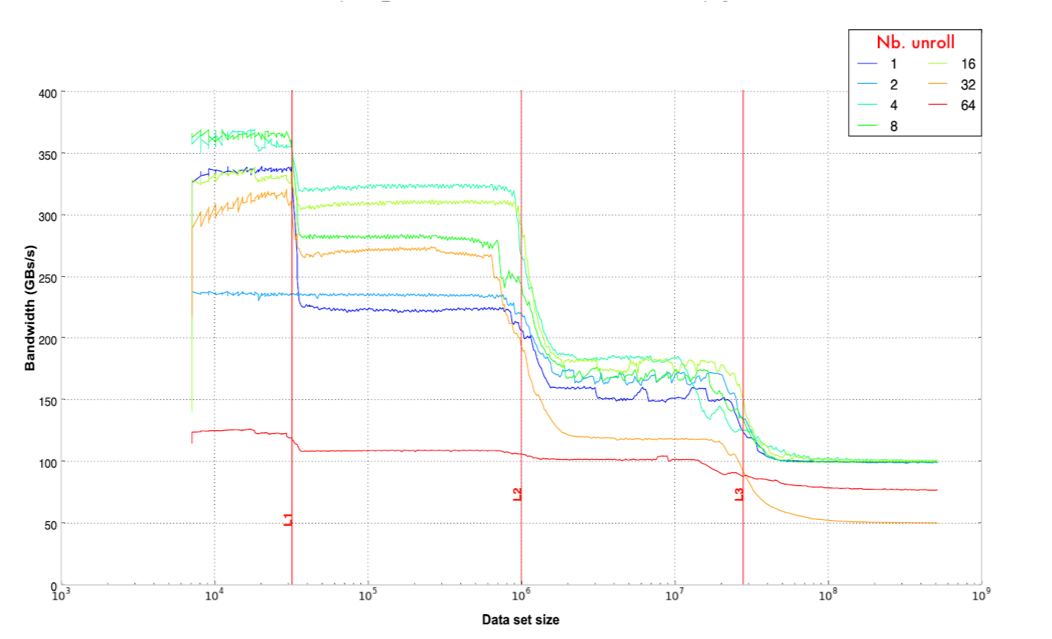
\includegraphics[width=16cm]{images/dml_unroll_best.png}
        \caption{\label{pic:dml_unroll_best} Performance de plusieurs déroulements pour une stride de 8 bytes (lecture de tous les éléments).}
        \end{figure}
        
    
    \subsubsection{Large page} \label{sec:dml_large_page}
    %%%%%%%%%%%%%%%%

    L'expérimentation suivante a pour objectif de comparer la performance du benchmark lors de l'utilisation de différentes tailles de pages mémoire. Comme présenté dans l'\aref{sec:page}, l'utilisation de page de plus grande taille permet d'améliorer la performance du système mémoire, notamment en accélérant le traitement de la TLB. Les pages plus larges permettent aussi de réduire les conflits d'associativité dans les caches. L'expérimentation réalisée avec un coeur actif a permis d'obtenir les résultats présentés dans le \autoref{tab:large_page_memory}. La performance des caches est améliorée avec l'utilisation des pages larges, jusqu'à 30\% dans le cache L3. Lorsque le jeu de données est dans le cache de niveau 3, la mesure du nombre d'évènements \textit{miss} de la TLB augmente d'un facteur 300. Cependant, la TLB arrive à masquer la majorité de ces \textit{miss} et conserve une bonne performance (150 GB/s).

    \begin{table}[]
    \centering
    %\resizebox{\textwidth}{!}{%
    \begin{tabular}{l|c|c|c|c|c|}
    \cline{2-6}
     & \cellcolor[HTML]{EFEFEF}L1 (GB/s) & \cellcolor[HTML]{EFEFEF}L2 (GB/s) & \cellcolor[HTML]{EFEFEF}L3 (GB/s) & \cellcolor[HTML]{EFEFEF}Memoire (GB/s) & \cellcolor[HTML]{EFEFEF}dTLB-load-misses \\ \hline
    \multicolumn{1}{|l|}{\cellcolor[HTML]{EFEFEF}Page de 4 KiB} & 320 & 220 & 150 & 13.40 & 2254025 \\ \hline
    \multicolumn{1}{|l|}{\cellcolor[HTML]{EFEFEF}Page de 2 MiB} & 340 & 225 & 200 & 13.45 & 6556 \\ \hline
    \end{tabular}%
    %}
    \caption{Performance du benchmark \texttt{DML\_MEM} utilisant deux tailles de pages. Le débit des 4 niveaux de la hiérarchie mémoire (GB/s) a été mesurée en utilisant une stride de 64 bytes. Le nombre d'évènements \textit{miss} correspond à l'exécution du benchmark avec un jeu de donnée situé dans le cache L3.}
    \label{tab:large_page_memory}
    \end{table}
    
    
    Nous nous sommes ensuite intéressés aux performances du benchmark lorsque plusieurs coeurs sont actifs, avec et sans l'utilisation des pages larges. Nous observons les mêmes écarts de performances lorsque le jeu de données est stocké dans les caches. Lors de l'utilisation de pages standards (4 KiB), nous constatons que lorsque la taille du jeu de données approche de la taille d'un niveau de cache, la performance commence à se détériorer. Avec l'utilisation des pages de 4 MiB, la performance dans chaque niveau de cache est constante et ne se détériore que lorsque le jeu de donnée dépasse la taille du niveau de cache. Cet effet observé lors de l'utilisation de petites pages est appelé \textit{page coloring}\footnote{La coloration de page est une technique logicielle permettant d'améliorer le mappage d'une page de la mémoire physique sur les lignes de cache du processeur. Cette technique permet d'assurer que des pages contiguës en mémoire virtuelle sont allouées à des pages physiques qui se répartiront efficacement dans les caches.} \cite{Zhang2009}.
  
    \begin{figure}
    \center
    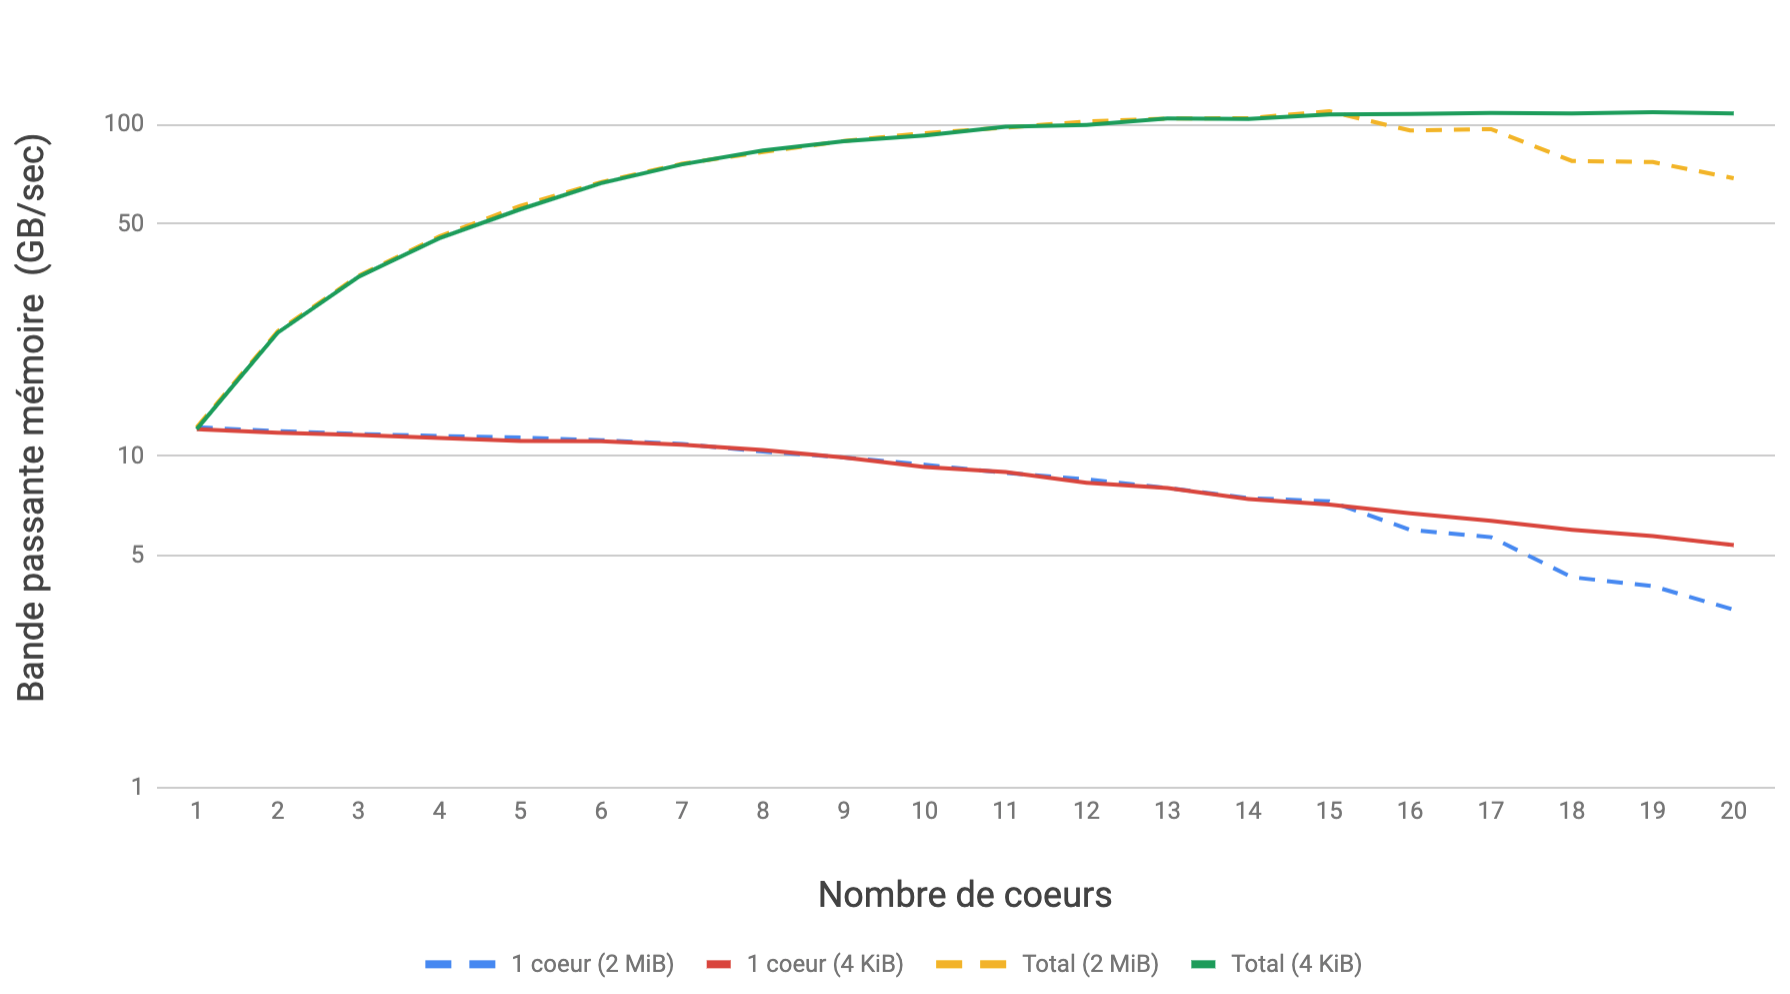
\includegraphics[width=14cm]{images/dml_large_page_bw.png}
    \caption{\label{pic:dml_large_page_bw} Débit mémoire mesuré en GB/s atteint par un coeur (rouge et bleu) et par différents nombre de coeurs (jaune et vert) utilisant des pages de 4 KiB (rouge et vert) et 2 MiB (bleu et jaune) pour accéder à un jeu de données de 2 GiB.}
    \end{figure}
    
    Le graphique de la \autoref{pic:dml_large_page_bw} montre les performances du benchmark avec un ou plusieurs coeurs actifs sur un jeu de donnée de 2 GiB. Nous remarquons que la performance du benchmark baisse lorsque plus de 15 coeurs sont utilisés avec des pages larges. La performance par coeur diminue de 5.39 GB/s à 3.44 GB/s alors que le bus mémoire n'est pas saturé. Nous n'avons pour le moment pas réussi à expliquer ce problème qui affecte tous les jeux de données supérieurs à 2 GiB.
    
    Bien que la TLB limite rarement les performances des applications réelles, le recours à l'utilisation de pages larges peut être bénéfique. Les versions récentes du noyau Linux peuvent choisir elles-mêmes lors de l'allocation mémoire si le recours à des pages plus grandes peut être bénéfique pour l'application (Red Hat Transparent Huge Pages (THP)). Comme nous montrons dans cette dernière expérience que l'utilisation de page de 2 MiB peut détériorer les performances, nous conseillons que cette responsabilité revienne à l'utilisateur qui devra décider ou non de leur utilisation en fonction de son application. 
  


    
    \subsubsection{Fréquence et coeurs: impact sur le débit mémoire} \label{sec:dml_core_vs_freq}
    %%%%%%%%%%%%%%%%
    
    Dans cette expérimentation nous avons mesuré la bande passante mémoire atteignable par notre benchmark pour différente configuration de fréquence et nombre de coeurs actifs. Les résultats sont visibles sur la \autoref{pic:dml_core_vs_freq}. Comme dans l'expérimentation précédente (\autoref{sec:dml_saturation}), nous démontrons que la totalité des coeurs n'est pas nécessaire pour saturer la bande passante. Cette expérience montre aussi que les coeurs utilisés n'ont pas besoin d'utiliser leur fréquence maximale. En effet, notre benchmark sature le bus mémoire avec 17 coeurs cadencés à seulement 2.1 GHz. Le script utilisé pour générer la \autoref{pic:dml_core_vs_freq} annote automatiquement le graphique pour identifier rapidement les maximums. Une telle utilisation du benchmark \verb=DML_MEM= permet d'identifier le couple  \verb|{fréquence, nombre de coeurs}| minimal pour saturer le bus mémoire. Pour des applications limitées par la performance de ce dernier, il peut être intéressant de désactiver les coeurs supplémentaires ou de plafonner la fréquence du processeur pour limiter la consommation électrique. En plus de vérifier la présence potentielle de bogues dans l'architecture, cette expérimentation peut permettre à un utilisateur de choisir la meilleure configuration pour un achat de nouveaux processeurs. 
    
    \begin{figure}[h!]
    \center
    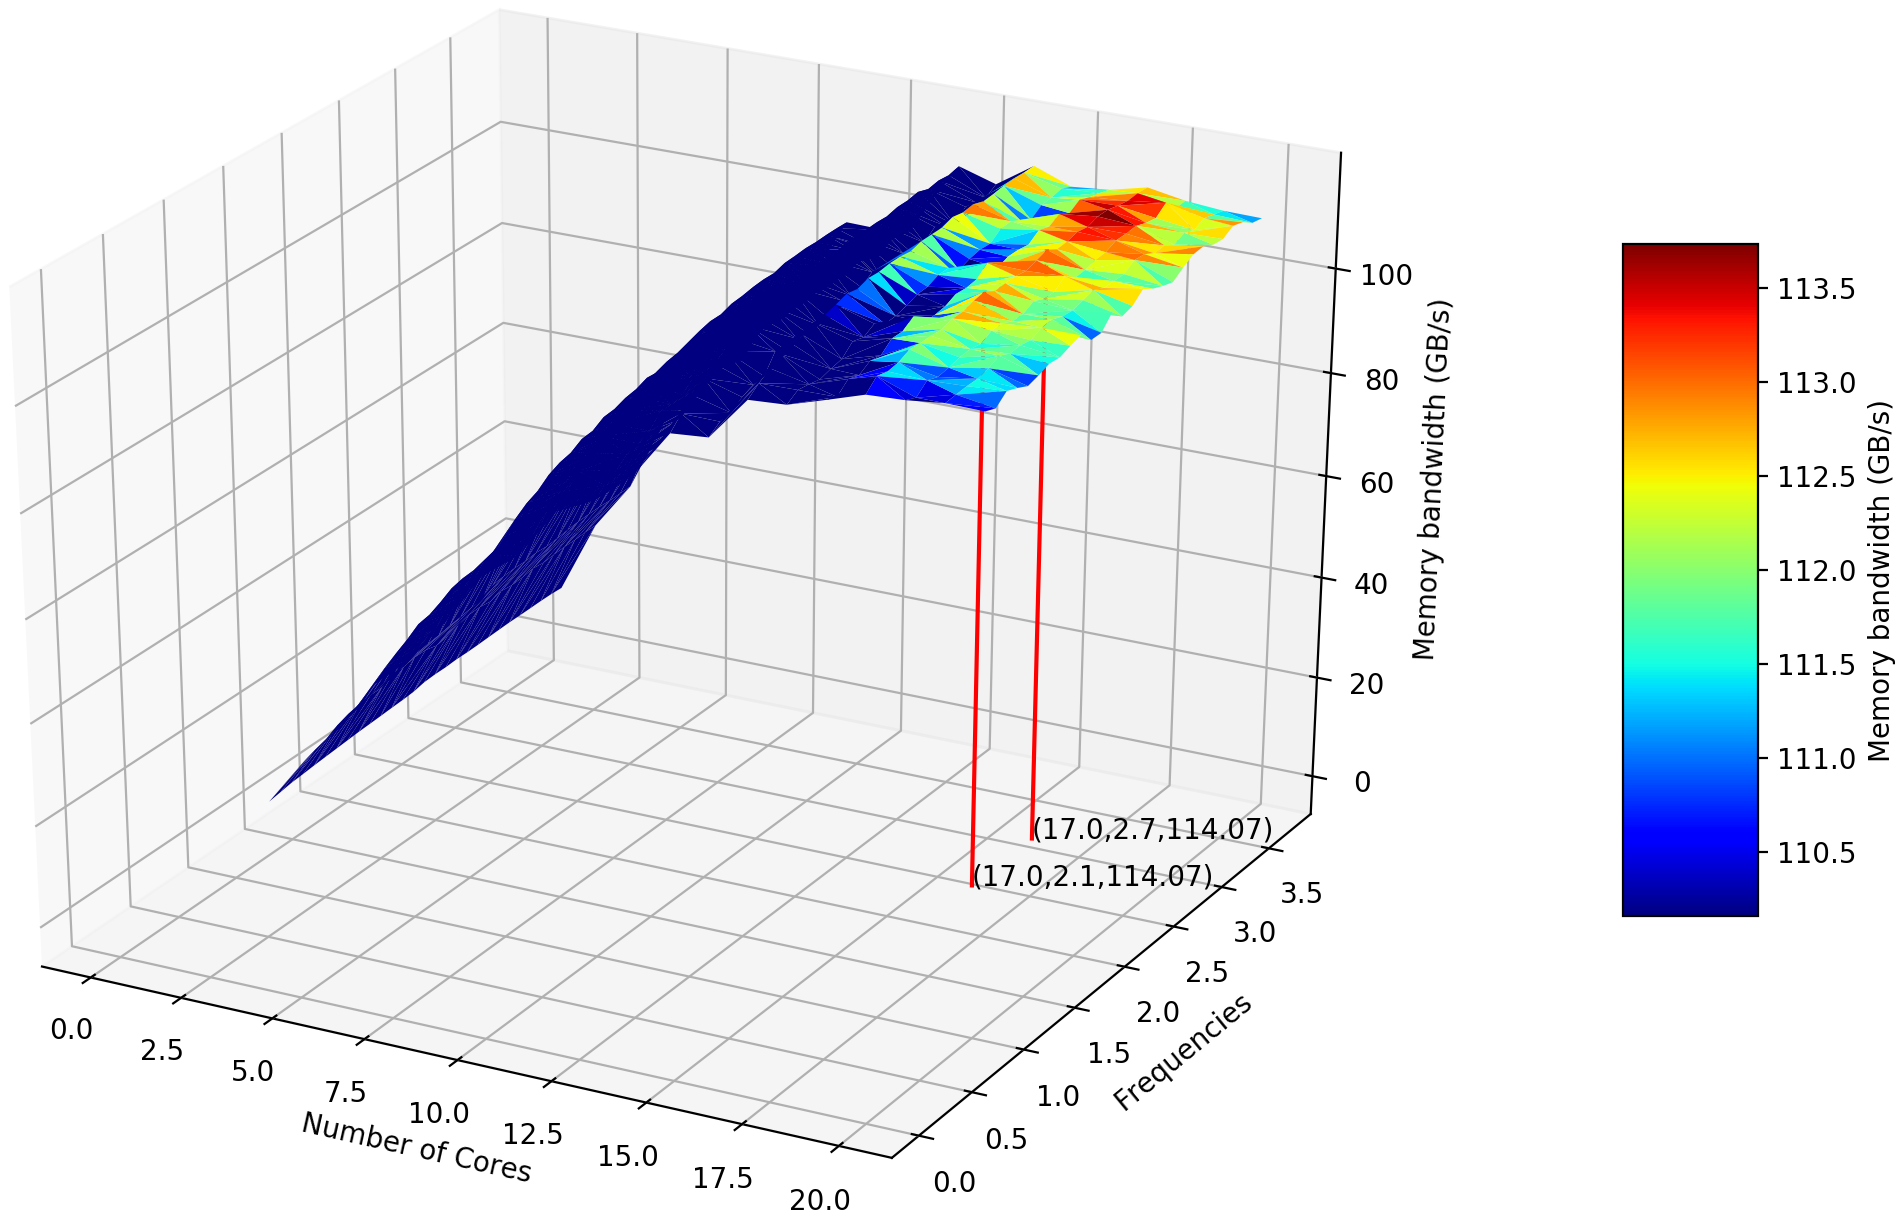
\includegraphics[width=14cm]{images/dml_core_vs_freq.png}
    \caption{\label{pic:dml_core_vs_freq}  Mesure du débit du bus mémoire (en GB/s) atteint par le benchmark lors de l'utilisation de différent nombre de coeurs dont la fréquence était limitée à différentes valeurs (en GHz). Le débit maximal atteint pour ce processeur est de 114.07 GB/s en utilisant 17 coeurs cadencés à 2,1 ou 2,7 GHz.}
    \end{figure}
    


    
    

\subsection{Conclusion}
%%%%%%%%%%%%%%%%%%%%%%%%%%%%%%%%%%%%%%%%%%%%%%%%%%%%%%

    Cette section s'intéresse au benchmark \verb=DML_MEM=, un outil permettant de caractériser de multiples parties du système mémoire. Le benchmark utilise des accès mémoire par saut, appelés \glspl{stride} et nous a permis de caractériser plusieurs parties de la microarchitecture. Une première utilisation nous a permis de déduire la taille d'une ligne de cache, donnée importante pour la programmation efficace d'applications. En utilisant différentes tailles de strides, nous avons pu mesurer l'impact que celles-ci pouvaient avoir sur la performance des différents niveaux de la hiérarchie mémoire. En utilisant une taille de stride correspondant à la taille d'une ligne de cache, nous avons pu caractériser l'architecture pour l'exécution d'algorithmes de streaming. Nous avons ainsi pu mesurer le débit maximal atteignable par le bus mémoire. Lors de nos expérimentations, nous avons obtenu des débits supérieurs (de l'ordre de 5\%) que ceux obtenus grâce au benchmark STREAM \cite{McCalpin1995}. Nous avons ensuite utilisé le benchmark \verb=DML_MEM= pour exposer la complexité des microarchitectures modernes. Nous montrons que la microarchitecture peut avoir des comportements inattendus lors de l'utilisation de certaines tailles de saut. À travers ces expérimentations nous souhaitons attirer l'attention du programmeur sur la complexité de la microarchitecture et de la nécessité de sa caractérisation. Nous avons pu voir que les performances atteintes par un code aussi simple pouvaient varier de plusieurs ordres de grandeur à cause de paramètres subtils: préchargement mémoire, taille des pages, nombre de déroulements de boucle...
    
    
    Lors des travaux de thèse, l'utilisation de cet outil nous a permis de caractériser plusieurs plateformes différentes et de déceler un bogue majeur dans un nouvel accélérateur. Ce bogue, inconnu par l'entreprise l'ayant conçue, condamne les applications utilisant des motifs de calculs de type Stencil, à n'accéder qu'à une fraction des performances mémoires théoriques de l'accélérateur. Ce travail réalisé pour un client industriel ne peut cependant pas être rendu public dans ce manuscrit.\newpage
        \section{Benchmark d'unité arithmétique}\label{sec:kg}


    Cette section présente un benchmark appelé \verb=Kernel Generator=. Cet outil permet de vérifier le bon comportement du matériel responsable de l'exécution des instructions de calculs sur des nombres à virgule flottante, utilisées par la grande majorité des applications HPC. L'exécution de ces opérations est réalisée par un composant, appelé unité de calcul en virgule flottante (ou \gls{FPU}), présentée dans la section suivante. Lorsque la performance des applications n'est pas limitée par celle du système mémoire, leur performance dépend essentiellement de celle des FPU. 



\subsection{Motivation et objectifs}
%%%%%%%%%%%%%%%%%%%%%%%%%%%%%%%%%%%%%%%%%%%%%%%%%%%%%
    
    La performance des applications sur des architectures modernes est principalement limitée par celle du système mémoire. Ainsi, les efforts de développement d'outils de caractérisation se sont en grande partie consacrés à la caractérisation de cette partie de l’architecture. Cependant, avec le développement de nouvelles architectures, la différence de performance entre les unités de calculs et celle du système mémoire devrait être plus équilibrée. Il est donc important d'avoir les outils nécessaires pour les caractériser.
    
    Bien que le comportement des FPU d'architectures actuelles soit connu, certaines particularités sont encore difficiles à caractériser: exécution dans le désordre et dépendances entre instructions (\aref{sec:out_of_order}) ou la fréquence atteignable pour un type d'instruction vectorielle (\aref{sec:frequency}).
    Il est nécessaire de connaître la performance maximale d'un processeur (mesurée par le nombre d'\gls{FLOP}) pour différents types de calculs. Celle-ci peut alors être utilisée pour apprécier les performances d'un code grâce à des modèles de type Roof line (voir \autoref{sec:roofline}). Afin d'obtenir le débit maximal de calculs réalisable par une architecture, deux approches peuvent être envisagées. La première utilise les caractéristiques matérielles pour la calculer. Cependant, la complexité des architectures nous a souvent montré que la performance réellement atteignable pouvait être différente (inférieure, mais parfois supérieure) des performances théoriques. La deuxième technique a recourt à des codes de \glspl{benchmark}. En utilisant des codes réels, il est alors possible de trouver des comportements cachés de l'architecture et d'en déceler des limitations.
    
    
    \subsubsection{Floating Point Unit (FPU)}
    %%%%%%%%%%%%%
        La \gls{FPU} est un composant majeur des ordinateurs et a connu de nombreuses évolutions au fil des générations. À l'origine, les FPU étaient des composants additionnels pouvant être ajoutés sur la carte mère pour accélérer l'exécution de calcul en virgule flottante (\autoref{pic_cpu_fpu}). C'est pour cela qu'il est commun de designer ce composant comme un accélérateur. Cependant, les applications réalisant de plus en plus de calculs de ce type, les FPU ont ensuite été directement intégrées au processeur (\autoref{pic_cpu_fpu_recent}). La FPU reçoit ses instructions du même décodeur que celui de l'\gls{ALU}. Lorsque les premiers étages du pipeline ont décodé l'instruction à exécuter (voir \autoref{sec:pipeline}), le séquenceur choisi si elle doit être exécutée par l'\gls{ALU} ou la \gls{FPU}. 
        
        \begin{figure}
            \centering
            \begin{subfigure}[b]{0.45\linewidth}
                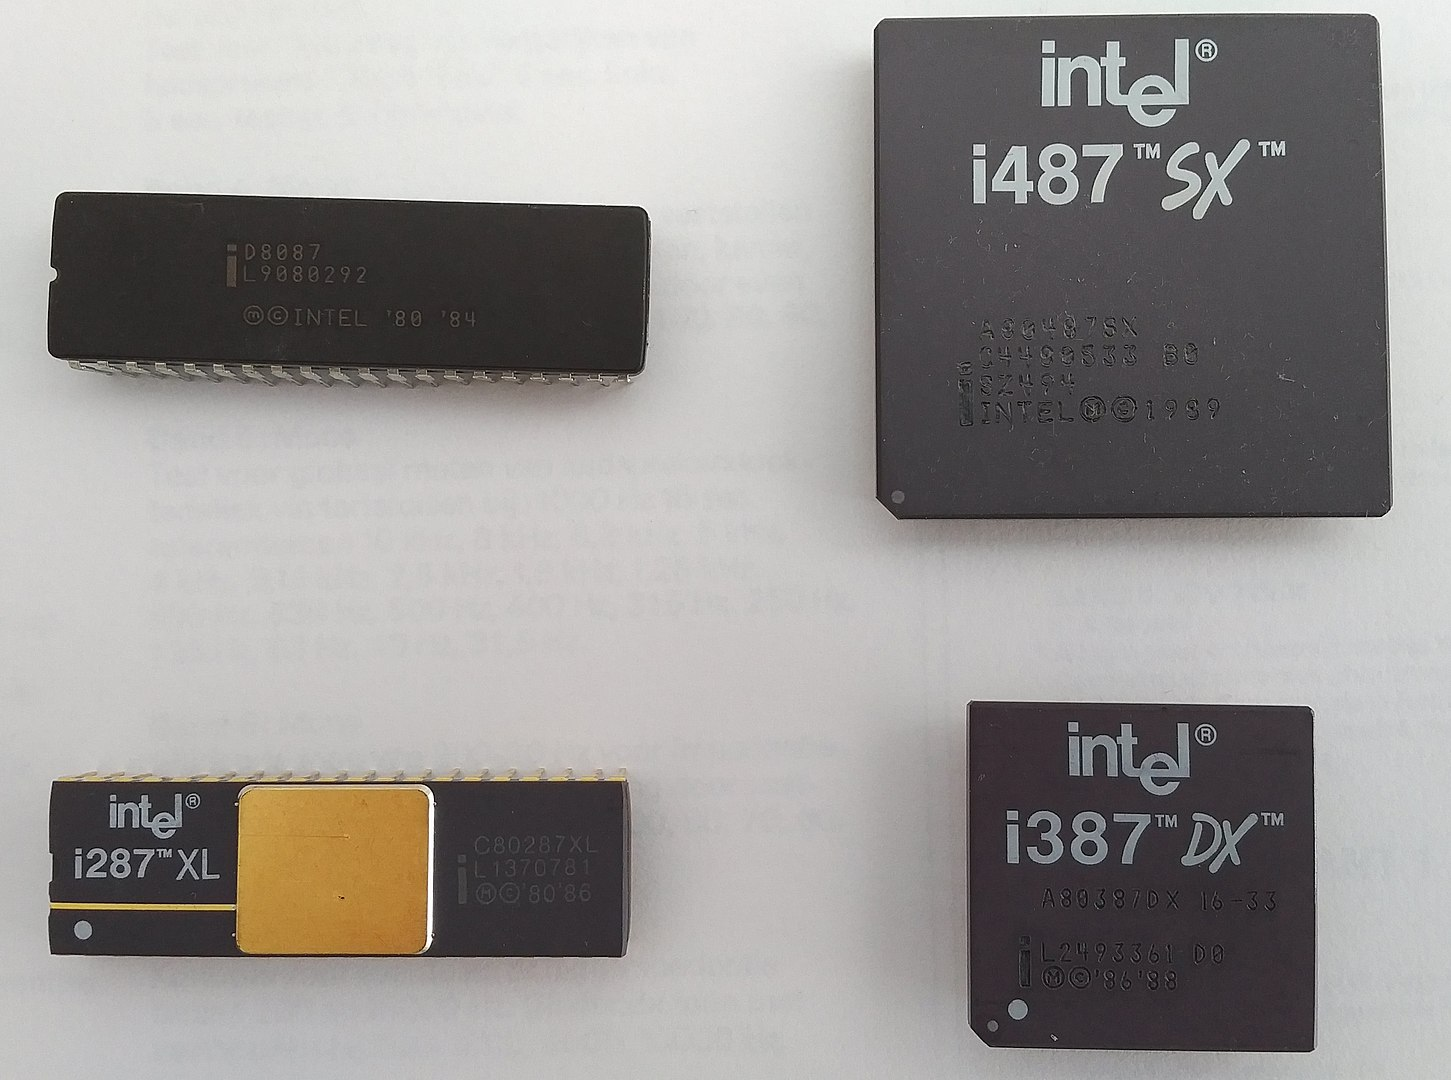
\includegraphics[width=\linewidth]{images/cpu_fpu.jpg}
                \caption{À l'origine, les FPU pouvaient être achetées séparément des processeurs.}
                \label{pic_cpu_fpu}
            \end{subfigure}
            ~ %add desired spacing between images, e. g. ~, \quad, \qquad, \hfill etc. 
              %(or a blank line to force the subfigure onto a new line)
            \begin{subfigure}[b]{0.45\linewidth}
                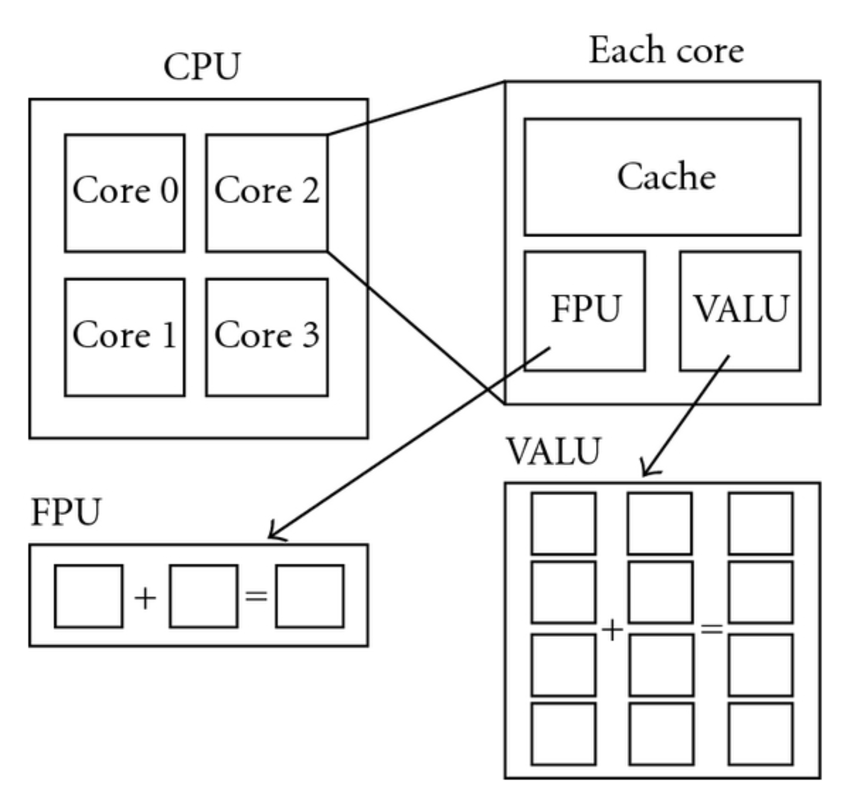
\includegraphics[width=\linewidth]{images/cpu_fpu_recent.png}
                \caption{Aujourd'hui, la FPU fait partie de chaque coeur du processeur.}
                \label{pic_cpu_fpu_recent}
            \end{subfigure}
            \caption{La FPU d'un processeur est un matériel permettant d'exécuter efficacement des instructions de calculs arithmétiques sur des nombres à virgule flottante: addition, soustraction, multiplication, division, racine carrée, etc...\protect\footnotemark }\label{fig:cacheinclusionpolicy}
        \end{figure}
        \footnotetext{Source images: \url{https://en.wikipedia.org/wiki/Floating-point_unit} et \url{https://www.extremetech.com/computing/263963-intel-reverses-declares-skylake-x-cpus-two-avx-512-units}}
        
        L'ajout de la FPU directement sur les coeurs a notamment permis de réduire les latences d'accès. De plus, avec l'apparition de plateformes multiprocesseurs, la gestion d'erreurs et d'exceptions liées aux FPU externes était devenue très difficile. Le premier processeur Intel à posséder une FPU et une ALU sur la même puce est le processeur Intel 80486DX produit en 1989.  Aujourd'hui, les FPU sont des composants de haute performance capable d'exécuter plusieurs instructions de calcul sur des nombres réels grâce à des instructions vectorielles.  

        
        
        Les applications de HPC réalisent majoritairement des calculs sur nombres à virgule flottante qui sont exécutés par les FPU. Ces unités sont très sollicitées et il est important d'en connaître les caractéristiques: débit, latence, fréquence maximale soutenable par le processeur. Les instructions vectorielles les plus longues utilisent plus de transistors pour être utilisées. Ainsi, la chaleur émise par le processeur varie et les instructions les plus complexes ne peuvent pas être exécutées aux fréquences maximales du processeur. Les différentes fréquences atteignables pour un type d'instruction peuvent être difficiles à prévoir.
        
        %Les modèles tels que celui du \textit{roof line} (voir \autoref{sec:roofline}), ont besoin de ces caractéristiques pour pouvoir comparer la performance mesurée d'une application à celle théoriquement atteignable. 
       
       
    \subsubsection{Objectifs}
    %%%%%%%%%%%%%
    \textbf{todo revoir les objectifs a la fin}
    
        Dans ce chapitre, nous présentons  un outil permettant de caractériser finement les performances des unités de calcul en virgule flottante (\gls{FPU}). Le développement de cet outil a été motivé par la nécessité d'obtenir différentes caractéristiques de la microarchitecture:
        \begin{enumerate}
            \item La première caractéristique pouvant être mesurée est la performance maximale atteignable par la FPU pour un certain type d'instruction. Cette performance est mesurée en \gls{FLOPS} et notée \gls{flopsmax}). Elle doit être mesurée pour des types et des tailles d'instructions vectorielles différents. L'avantage de cette unité est de rendre les résultats du Kernel Generator comparable avec ceux d'autres benchmarks (tel que \textit{HPL} \cite{Dongarra2003}).
            
            \item La deuxième caractéristique mesurable est la latence des instructions. Il peut être intéressant de connaître celle-ci lors de l'exécution d'instructions dépendantes.
            
            \item D'autres comportements doivent être caractérisés pour anticiper et comprendre la performance de certaines applications. Parmi eux, celui de l'unité d'exécution dans le désordre. Certains codes comportant beaucoup de dépendances sont limités par la faculté du processeur à exécuter plusieurs chaînes de dépendances. 
        
        \end{enumerate}
 
        
\subsection{Kernel Generator}    
%%%%%%%%%%%%%%%%%%%%%%%%%%%%%%%%%%%%%%%%%%%%%%%%%%%%%

        Afin de répondre aux objectifs fixés dans la section précédente, nous proposons l'outil \verb=Kernel Generator=. Il permet de générer des \gls{kernel} en assembleur pour caractériser finement le comportement des \gls{FPU}. Cet outil vise plus particulièrement les développeurs d'application dont la performance est limitée par le débit d'exécution d'instructions de calcul (\gls{computebound}). Bien que la performance des processeurs soit souvent limitée par la bande passante mémoire, une partie significative des codes est purement \gls{computebound}. 
        
        L'outil du \verb=Kernel Generator= permet de mesurer certaines caractéristiques de la FPU d'un processeur grâce à l'exécution d'un kernel généré en assembleur comportant des instructions de calcul arithmétique. Les instructions utilisées peuvent être scalaires ou vectorielles. La version actuelle de l'outil supporte les instructions de types scalaire, SSE, AVX2 et AVX512. 
            
        Grâce à ses différentes options, l'utilisateur peut générer des kernels d'instructions de types et de tailles différents. La valeur de l'outil vient de son utilisation et des différents tests que le programmeur peut réaliser. L'outil peut aussi être utilisé pour détecter des problèmes de la microarchitecture lors de l'exécution intensive d'instructions de calculs. Détecter ces comportements cachés peut ensuite permettre de mieux apprécier la performance d'une application réelle. 
            

        
        

    \subsubsection{Concept}
    %%%%%%%%%%%%%%%%%%%%%%
        L'outil du \verb=Kernel Generator= est un générateur de code assembleur permettant de mesurer la performance de la FPU d'un coeur de processeur. Pour cela, l'outil génère automatiquement un programme en langage C++ contenant:
        \begin{itemize}
            \item Les instructions assembleurs sélectionnées par l'utilisateur. 
            \item Le code responsable de l'exécution et des différentes mesure de performance
        \end{itemize}
                    \begin{figure}
            \center
            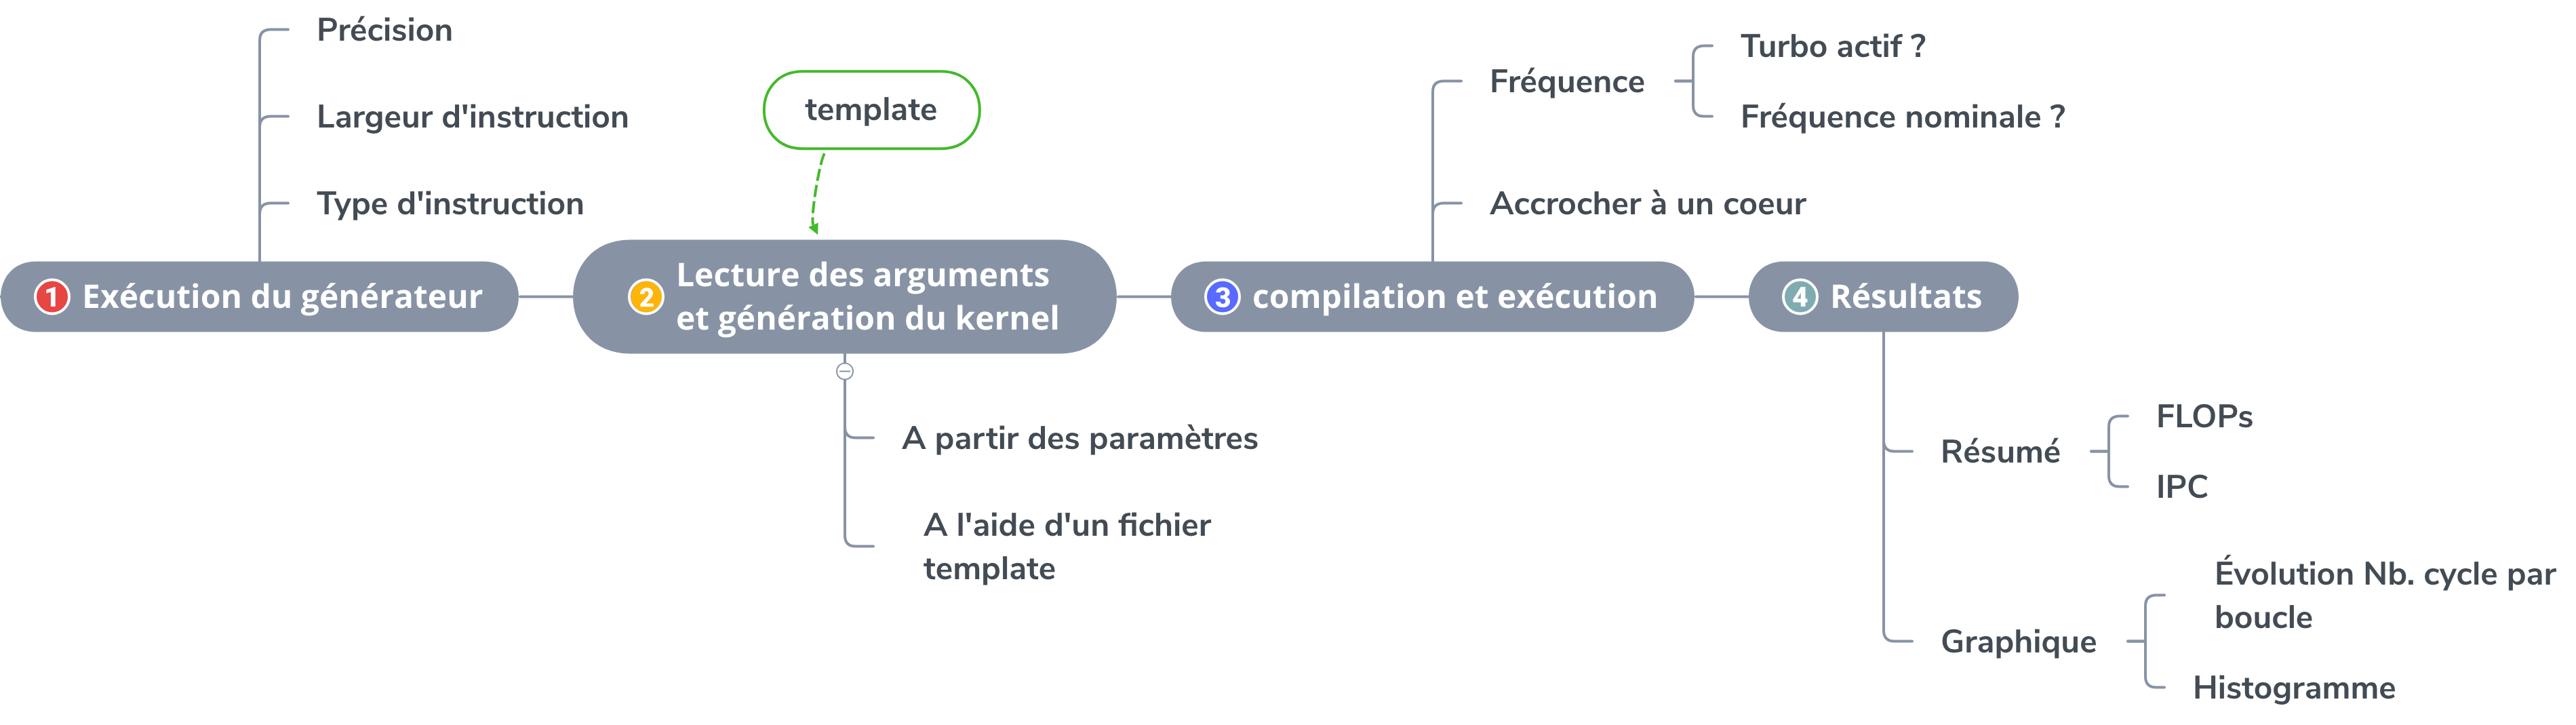
\includegraphics[width=17cm]{images/kg_workflow.png}
            \caption{\label{pic_kg_workflow} Déroulement de l'exécution du générateur de kernels.}
            \end{figure}
        La \autoref{pic_kg_workflow} montre les étapes principales de l'utilisation du générateur de kernel. Le code généré par l'outil reste simple pour faciliter les conclusions que pourra tirer son utilisateur. En effet, produire un code trop complexe rendrait l'analyse des résultats trop difficile sur des  architectures aussi complexes que celles étudiées. Un exemple d'utilisation de l'outil peut être réalisé grâce à la commande suivante:\\
        \verb|./kg   -P double -W 128  -O aamm|\\
        Cette commande permet de générer un kernel de calculs utilisant quatre instructions vectorielles de 128 bits sur des nombres flottants en double précision. Le kernel généré est présenté dans l'\autoref{code_kg_exemple}. Il composé de quatre instructions: deux additions et deux multiplications.
        
\begin{minipage}{0.97\linewidth}
\begin{lstlisting}[label=code_kg_exemple ,language=, caption=Exemple de kernel généré à l'aide de la commande \texttt{./kg   -P double -W 128  -O aamm} contenant 4 instructions vectorielles de 128 bits.]
"vaddpd %%xmm0, %%xmm1, %%xmm2;"
"vaddpd %%xmm0, %%xmm1, %%xmm3;"
"vmulpd %%xmm0, %%xmm1, %%xmm4;"
"vmulpd %%xmm0, %%xmm1, %%xmm5;"
\end{lstlisting} 
\end{minipage}

        À partir des arguments, le générateur écrit un programme en langage C++ qu'il compile et exécute. Les résultats sont ensuite présentés sous forme de texte dans le terminal ou sous forme de graphique (nécessite python).
        Le choix du langage assembleur a été motivé par la volonté de s'assurer que les instructions générées étaient bien exécutées. En effet, les compilateurs deviennent toujours plus performants et optimisent les codes rendant l'analyse de performance plus difficile. De plus, ils peuvent comprendre l'artificialité d'un code et contourner son exécution. En générant nous même le code assembleur, nous nous assurons que la performance du code mesuré est bien celle attendue.
    
       
    \subsubsection{Les options.}\label{sec:kg_option} 
    
        Une des forces du générateur vient de sa capacité à générer un grand nombre de benchmarks différents. Ceci est possible grâce à l'utilisation des différentes options dont les principales sont listées ci-dessous:
    
        \paragraph{\texttt{-{}-operation [a,m,f]+}} Lister les opérations à réaliser par le kernel à l'aide d'une chaîne de caractères composé des lettres \texttt{a}, \texttt{m} et \texttt{f} correspondant aux opérations suivantes : addition (a), multiplication (m) ou \gls{FMA} (f). Différentes opérations peuvent être mixées et seront insérées dans le \gls{kernel} dans le même ordre. Un script externe peut alors être utilisé pour générer des kernels testant différentes combinaisons d'opérations. En faisant varier à la fois les opérations et la taille des instructions, l'outil permet de découvrir des comportements cachés des architectures.

        \paragraph{\texttt{-{}-precision (single | double)}} Définir la précision utilisée pour réaliser les calculs: simple ou double. Pour le moment, des instructions ayant des précisions différentes ne peuvent pas être mixées dans un même kernel.
        
        \paragraph{\texttt{-{}-width (64 | 128 | 256 | 512)}} Définir la \textit{largeur} des instructions vectorielles utilisées. Sur une architecture Intel, ces instructions correspondents aux ISA suivantes: MMX (64), SSE (128), AVX (256) et AVX-512 (512). Pour le moment, des instructions vectorielles de tailles  différentes ne peuvent pas être mixées dans un même kernel.
        
        \paragraph{\texttt{-{}-dependency N}} Générer une instruction  dont un opérande est le résultat produit par l'instruction précédente. Un nombre \texttt{N} peut être donné pour générer plusieurs chaînes de dépendances. Cette option est particulièrement utile pour mesurer la latence des instructions et la performance du tampon d'exécution dans le désordre.
        
        \paragraph{\texttt{-{}-binding N}} Accrocher (\textit{bind}) le benchmark généré à un coeur spécifique. Le benchmark n'étant pas parallélisé il est nécessaire d'en exécuter plusieurs versions en parallèle pour tester la performance d'un processeur lorsque plusieurs coeurs sont utilisés. Les différents processus crées peuvent alors être \textit{accrochés} aux différents coeurs du processeur à l'aide d'un script externe.
        
        \paragraph{\texttt{-{}-unroll N}} Appliquer l'optimisation du déroulement de boucle \texttt{N} fois. Cette optimisation permet de dérouler plusieurs fois le corps de la boucle à l'intérieur de celle-ci pour réduire l'impact du traitement des instructions de contrôle de la boucle (incrémentation et comparaison) sur les performances du benchmark. 
        
        \paragraph{\texttt{-{}-frequency (true | false)}} Générer exécuter une fonction en début de benchmark qui mesure la fréquence du processeur. Les calculs des résultats sont impactés par l'utilisation du mode turbo. En connaissant la valeur de la fréquence turbo, ces résultats peuvent être ajustés. En effet, la mesure de la performance du benchmark est réalisée en utilisant la valeur de la fréquence de base du processeur. 
        
        \paragraph{\texttt{-{}-loopsize N}} Améliorer la précision des résultats et éliminer les potentiels bruits de mesure en réalisant \texttt{N} mesures.
    
    
    \subsubsection{Fonctionnement du générateur}
    %%%%%%%%%%%%%%%%%%%%%%
        
        Une fois les différentes options analysées, le générateur va écrire un programme C++ contenant le benchmark à exécuter. Tous les benchmarks ont une partie commune de code qui est stockée dans un fichier \textit{template}. Le générateur s'occupe seulement d'écrire la partie en assembleur dans ce fichier et d'initialiser quelques variables (nombre de mesures, coeur sur lequel s'exécuter). Le \textit{template} contient le code permettant de mesurer les résultats, de calculer la fréquence et d'afficher le résultat  dans le terminal. Un exemple d'exécution du générateur est résumé sur la \autoref{pic_kg_generation}. 

        \begin{figure}[h!]
            \center
            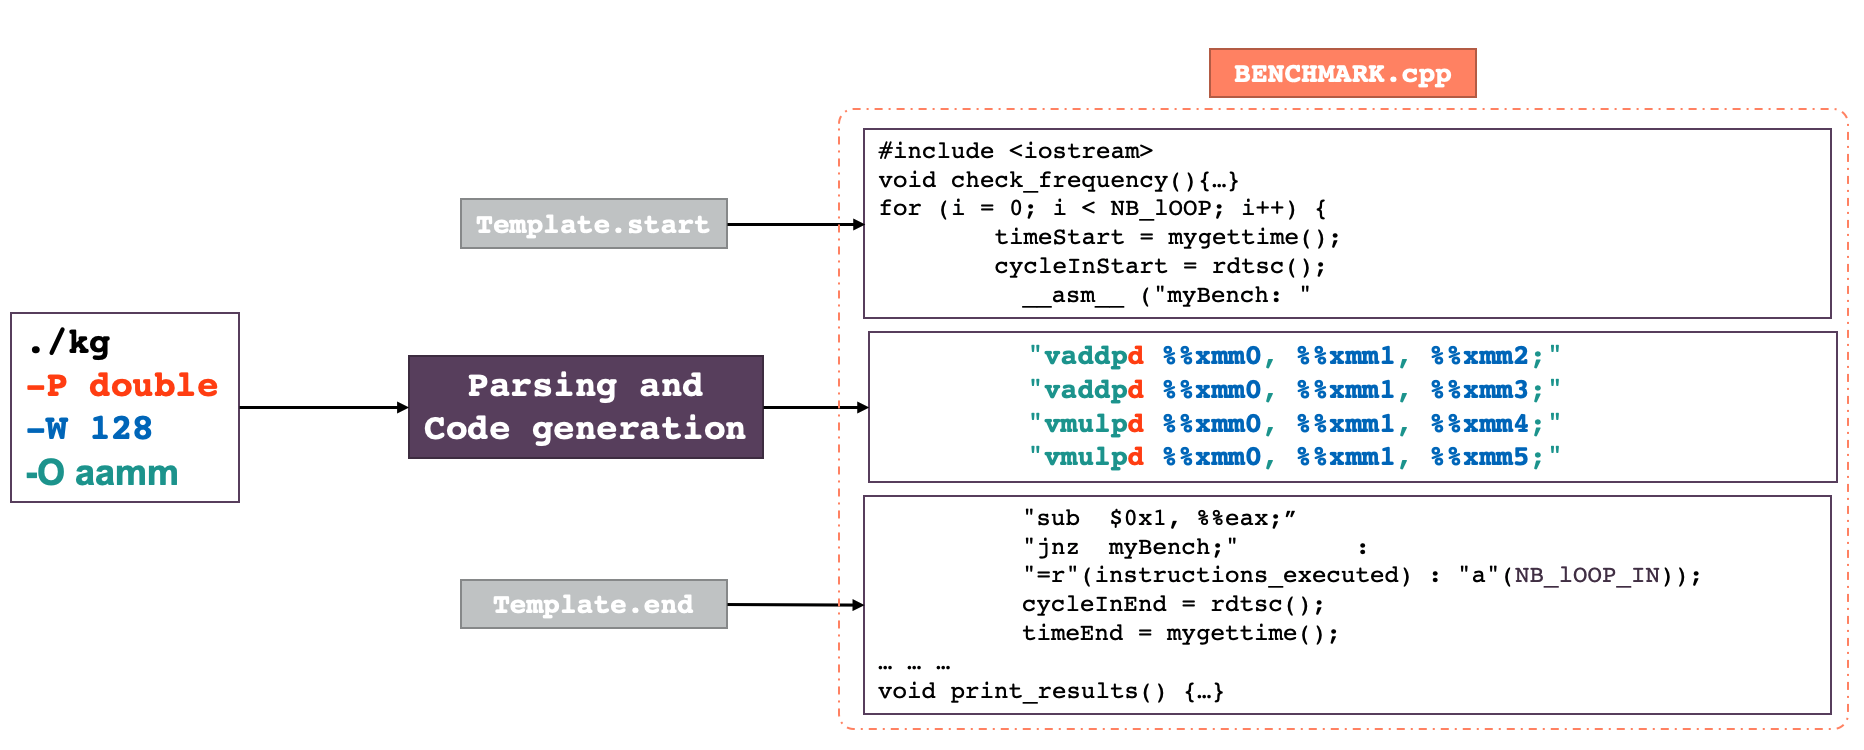
\includegraphics[width=14cm]{images/kg_generation.png}
            \caption{\label{pic_kg_generation}Génération du benchmark à partir de la ligne de commande entrée par l'utilisateur. La partie commune du code est stockée dans un fichier de \textit{template}.}
        \end{figure}
        
        Lorsque le code du benchmark généré, celui-ci est compilé automatiquement par le générateur (le compilateur utilisé peut facilement être modifié). Ces deux fichiers (le fichier source et l'exécutable) sont créés dans le dossier courant de l'utilisateur. L'exécutable peut ensuite être utilisés sans passer de nouveau par le générateur. Un exemple de résultat de l'exécution du benchmark est présenté dans l'\autoref{output:basic_gflops}.
    
 \begin{minipage}{0.97\linewidth}
 \begin{lstlisting}[label=output:basic_gflops ,language=, caption=Exemple d'exécution d'un benchmark de quatre instructions AVX-512.]
./kg -W 512 -O aamm -P double -U 4 -S 30000 -L 500000

--------------------  CHECK FREQUENCY  ------------------------
+ Base      frequency is 2.69GHz
+ Current   frequency is 2.68GHz
+ OK: the core is running at his frequency based value

------------------  INSTRUCTIONS SUMMARY -----------------------
_label_|   NB INSTRUCTIONS      Time    FREQUENCY   Giga_inst/sec     IPC
_value_|      240000000000      44.7         2.69            5.37    1.99

----------------------  FLOP SUMMARY  --------------------------
 PRECISION     FLOP/cycle         FLOP/second
    Single              0                   0
    Double             16             4.3e+10
----------------------------------------------------------------


\end{lstlisting}   
 \end{minipage}   
        Le benchmark généré comporte quatre instructions vectorielles AVX-512: deux additions et deux multiplications. Le processeur utilisé est un  Intel Xeon 6150 cadencé à 2.70GHz. Pour cette expérimentation le turbo a été désactivé. Pour améliorer la précision des résultats, la boucle générée est déroulée 4 fois. La boucle réalise 500000 itérations et sa performance est mesurée 30000 fois. Le CPU est capable d'exécuter deux opérations flottantes vectorielles par cycle d'horloge. Pour des données en doubles précisions, cela correspond à réaliser 16 opérations flottantes par cycle. La puissance de calcul atteinte par l'exécution du benchmark sur un coeur est de 43 GFLOPS . Pour chaque mesure le nombre de cycles et le temps nécessaire à l'exécution de la boucle sont sauvés dans un fichier. Ce fichier peut ensuite être affiché avec un script python (voir \autoref{fig:kg_graph}). La \autoref{pic_kg_plot} permet de voir comment la performance du benchmark évolue au fil des exécutions. On peut détecter des problèmes de détérioration des performances pouvant être dus à un mauvais refroidissement du processeur par exemple.  La \autoref{pic_kg_hist} affiche l'histogramme permettant de voir deux familles de performances. Dans cet exemple, la différence entre ces deux familles est inférieure à 0,02\%. Il peut cependant arrivé que pour certaines architectures, le processeur ne soit pas capable de maintenir une performance constante lors de l'exécution de certaines instructions. Ce comportement pourra alors être mis en évidence grâce à ce graphique.
        
        \begin{figure}
            \centering
            \begin{subfigure}[b]{0.45\linewidth}
                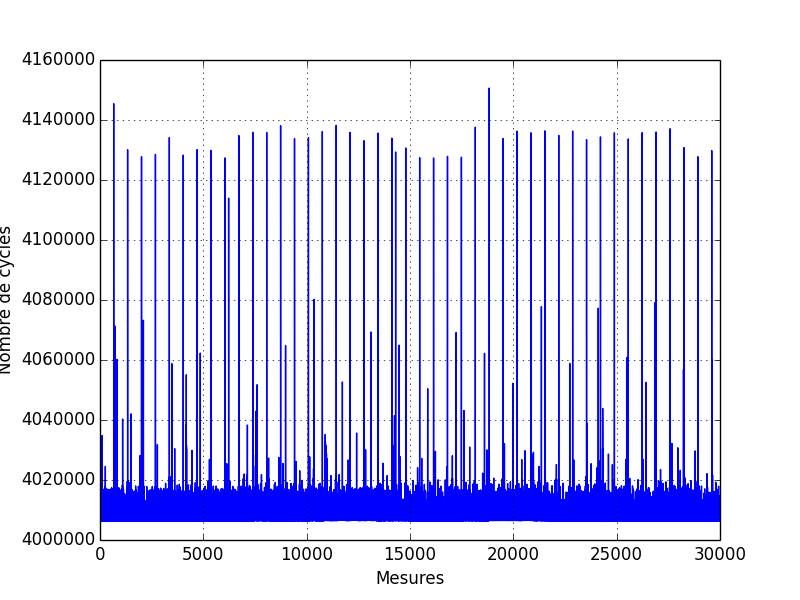
\includegraphics[width=\linewidth]{images/kg_plot.png}
                \caption{Évolution du nombre de cycles nécessaire pour l'exécution de la boucle de benchmark}
                \label{pic_kg_plot}
            \end{subfigure}
            ~ %add desired spacing between images, e. g. ~, \quad, \qquad, \hfill etc. 
              %(or a blank line to force the subfigure onto a new line)
            \begin{subfigure}[b]{0.45\linewidth}
                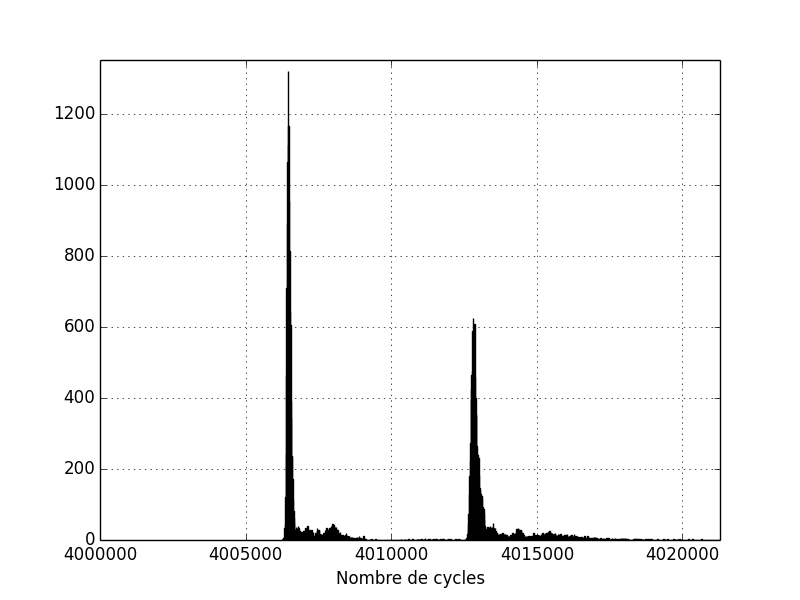
\includegraphics[width=\linewidth]{images/kg_hist.png}
                \caption{Histogramme du nombre de cycles nécessaire}
                \label{pic_kg_hist}
            \end{subfigure}
            \caption{Grâce à un script python, le fichier de résultat peut être affiché sous forme de graphique. }\label{fig:kg_graph}
        \end{figure}
    
  
        %%%% OPTION %%%    
    
    
    \subsubsection{Validation des résultats}
    
        Lors du développement du générateur, il a été nécessaire d'utiliser des outils nous permettant de valider les performances rapportées par le benchmark. Pour s'assurer du bon fonctionnement du benchmark sur de nouvelles architectures, certaines de ces méthodes de vérification ont été implémentées dans l'outil directement. 
        
        %#TODO enelver le compteur je pense qu'il est NDA pour HPE
        \paragraph{Validation du nombre d'instructions.} 
            
            La première valeur à valider est de s'assurer que le bon nombre d'instructions a été exécuté par le benchmark. Le benchmark affiche le nombre d'instructions qui devrait être exécuté. Un moyen de le vérifier est d'utiliser les compteurs matériels. L'outil \textit{perf} permet de mesurer le nombre d'évènements d'un compteur en utilisant son adresse. La ligne de commande suivante permet de compter les opérations flottantes réalisées par le benchmark: \verb|perf stat -e /rffc7 ./benchmark|. Le résultat du benchmark ci-dessus prévoyait l'exécution de 240,000,000,000 opérations. La commande \verb|perf stat| retourne une valeur de 240,000,210,024 opérations (une instruction FMA compte pour deux). Pour comprendre d'où proviennent les instructions supplémentaires, nous avons mesuré différentes versions du benchmark avec différentes longueurs de boucle (5000, 10000 et 20000). Le \autoref{tab:kg_vs_perf} donne les résultats affichés par le benchmark et par la commande précédente utilisant l'outil \textit{perf}. Les résultats de \textit{perf} mesurent le bon nombre d'instructions avec 2124 opérations supplémentaires à chaque fois. Ces instructions supplémentaires correspondent au traitement des résultats.
    
            \begin{table}[h!]
            \centering
            %\resizebox{\textwidth}{!}{%
            \begin{tabular}{@{}lcc@{}}
            \toprule
             Commande utilisée & Nombre d'instructions attendu & Résultat perf \\ \midrule
            ./kg -W 512 -O aamm -S 300 -L 5000 & 6000000 & 6002124 \\
            ./kg -W 512 -O aamm -S 300 -L 10000 & 12000000 & 12002124 \\
            ./kg -W 512 -O aamm -S 300 -L 20000 & 24000000 & 24002124 \\ \bottomrule
            \end{tabular}%
            %}
            \caption{Vérification du nombre d'instructions exécutées avec l'outil perf.}
            \label{tab:kg_vs_perf}
            \end{table}
        
        
        \paragraph{Validation de l'IPC.} 
        
            La validation du nombre d'\gls{IPC} du processeur peut elle aussi être réalisée grâce à perf: \verb|perf stat ./benchmark|. Pour générer le benchmark la commande suivante a été utilisée:\\
            \verb|./kg -W 512 -O aamm -P double -S 1000 -L 90000000|\\
            Lors de son exécution, le benchmark donne un IPC de 2 alors que la commande \textit{perf} donne un résultat de 3. Cette différence peut être expliquée en regardant le code assembleur généré (voir \autoref{lst:kg:ipc}).
        
\begin{minipage}{0.965\linewidth}
        \begin{lstlisting}[label=lst:kg:ipc ,language=C, caption={Code généré par la commande ./kg -W 512 -O aamm -P double. Le benchmark mesure la performance du la boucle à l'aide du compteur de cycle (\texttt{rdtsc()}). Cette mesure comprend l'exécution des instructions de calculs du kernel mais aussi les deux instructions de la gestion de boucle \texttt{sub} et \texttt{jnz}.}]
cycleInStart = rdtsc();
__asm__ ("" 
    "myBench: " 
		"vaddpd %%zmm0, %%zmm1, %%zmm2; "
		"vaddpd %%zmm0, %%zmm1, %%zmm3; "
		"vmulpd %%zmm0, %%zmm1, %%zmm4; "
		"vmulpd %%zmm0, %%zmm1, %%zmm5; "
    "sub  $0x1, %%eax;"
    "jnz  myBench;"		: "=r" (instructions_executed) : "a" (NB_lOOP_IN));
cycleInEnd = rdtsc();
\end{lstlisting}
\end{minipage}\\
            Le résultat donné par le benchmark ne prend en considération que les quatre instructions de calculs pour calculer l'IPC alors que l'outil \textit{perf} compte la totalité des instructions exécutées. Notre calcul prend pour postulat que les deux instructions de gestion de boucle (la décrémentation \verb|sub|, et le saut conditionnel \verb|jnz|) ne rentre pas dans le profil de l'exécution. En effet, grâce au prédicateur de branchement, l'instruction de saut peut effectivement être enlevée de nos calculs. 

            Concernant la soustraction, nous avons réalisé un test pour vérifier l'impact de soustraction de nombre entier lors de l'exécution d'un code ne réalisant que des opérations sur des nombres flottants (voir \autoref{code:sub}). En mesurant la performance de ce code, nous avons mesuré que 4 soustractions sur des nombres entiers n'impactent pas la performance de la boucle. Au-delà de 4, le processeur a besoin de cycles supplémentaires pour les exécuter. Ainsi les deux instructions de gestion de boucles peuvent être ignorées dans calcul. Pour réduire l'impacte de ces deux instructions sur le résultat donnée par \textit{perf}, nous avons implémenté une option de déroulement de boucle (\textit{unrolling}). En utilisant l'option \verb|-U 10|, le benchmark généré déroule la boucle 10 fois permettant de réduire l'impact des instructions de la gestion de boucle (incrémentation et test). Grâce à cette option, nous avons pu valider l'IPC calculé par notre benchmark avec celui mesuré par \verb|perf| (2 instructions par cycle).
        
            \begin{minipage}{0.965\linewidth}         \begin{lstlisting}[label=code:sub ,language=C, caption={En ajoutant jusqu'à 3 soustractions, nous avons pu vérifier que la soustraction utilisée pour la gestion de la boucle n'avait aucun impact sur la performance du benchmark. En effet, la soustraction sur un nombre entier n'utilise pas la FPU.}]
cycleInStart = rdtsc();
__asm__ ("" 
    "myBench: " 
       "vaddpd %%zmm0, %%zmm1, %%zmm2; "
       "vaddpd %%zmm0, %%zmm1, %%zmm3; "
       "vmulpd %%zmm0, %%zmm1, %%zmm4; "
       "vmulpd %%zmm0, %%zmm1, %%zmm5; "
       "sub  $0x1, %%ebx;" //soustraction artificielle
       "sub  $0x1, %%ebx;" //soustraction artificielle
       "sub  $0x1, %%ebx;" //soustraction artificielle
    "sub  $0x1, %%eax;"
    "jnz  myBench;"		: "=r" (instructions_executed) : "a" (NB_lOOP_IN));
cycleInEnd = rdtsc();
\end{lstlisting} \end{minipage}
        
        
        \paragraph{Validation des FLOPS.} 
            Afin de valider le nombre de calculs réalisés, deux méthodes ont été employées.
            La première méthode fut l'utilisation d'un outil développé en interne appelé \verb=mygflops=. Cet outil affiche le nombre d'opérations exécutées en consultant les compteurs matériels de chaque coeur. Le résultat sépare les différentes tailles d'instructions vectorielles utilisées. La commande, le résultat du benchmark et celui de \verb=mygflops= sont présentés dans l'\autoref{lst:basic_gflops}. 
        
\begin{minipage}{0.97\linewidth}         \begin{lstlisting}[label=lst:basic_gflops ,language=C, caption={L'utilisation de l'outil \texttt{mygflops}, développé par notre équipe, a permis de valider les résultats donnés par notre benchmark (\textit{ligne 6}). L'outil \texttt{mygflops} utilise les compteurs matériels pour mesurer les différentes instructions de calculs réalisées et permet de valider nos résultats (\textit{ligne 19}).}]
./kg -W 128 -O aamm -P double -U 10 -S 10 -L 90000000
...
----------------------  FLOP SUMMARY  --------------------------
 PRECISION     FLOP/cycle         FLOP/second
    Single              0                   0
    Double           4.00            1.06e+10
----------------------------------------------------------------
...

********************** MYGFLOPS ***********************
     
Single-precision SSE/AVX :            0.000000 GFlop/s --  0.0% of Flops

       0.0%  32-bit SSE/AVX instructions (0.0%)
       0.0% 128-bit SSE/AVX instructions (0.0%)
       0.0% 256-bit AVX instructions     (0.0%)
       0.0% 512-bit AVX instructions     (0.0%)
     
Double-precision SSE/AVX :            10.572521 GFlop/s -- 100.0% of Flops

       0.0%  64-bit SSE/AVX instructions (  0.0%)
     100.0% 128-bit SSE/AVX instructions (100.0%)
       0.0% 256-bit AVX instructions     (  0.0%)
       0.0% 512-bit AVX instructions     (  0.0%)

\end{lstlisting} \end{minipage}
        
        Malheureusement, l'outil \verb=mygflops= n'est pas disponible en accès libre pour le reste de la communauté. Nous avons ainsi développé une méthode de validation des résultats interne au benchmark. En fonction des opérations utilisées, les registres sont initialisés avec différentes valeurs significatives. Par exemple, pour vérifier que le bon nombre d'additions a été exécuté, les registres sont initialisés à la valeur 1. À la fin du benchmark, les registres ayant participé au benchmark sont sommés pour vérifier que le bon nombre d'additions a été exécuté. Grâce à cette méthode, nous avons la certitude que les opérations sont réellement exécutées par le processeur et qu'aucune optimisation lui permettant d'en éviter n'est possible ou une erreur de logique.
        

    \subsubsection{Mesure de la fréquence}
    %%%%%%%%%%%%%%%%%%%%%%
        Plus un processeur utilise une fréquence élevée, plus sa consommation électrique est élevée. Pour cette raison, Intel a adopté différents niveaux de fréquences pour ses processeurs. Cela permet d'augmenter les performances en cas de besoin et de limiter la consommation d'énergie si le processeur n'a pas besoin d'être pleinement utilisé. Les instructions les plus complexes (instructions vectorielles) nécessite l'utilisation de plus de transistors que les instructions scalaires. L'énergie dissipées est alors plus élevée, empêchant le processeur d'utiliser sa fréquence maximale pour l'exécution de telles instructions (voir \autoref{fig:cpu_freq_avx}). 
        
        \begin{figure}
            \center
            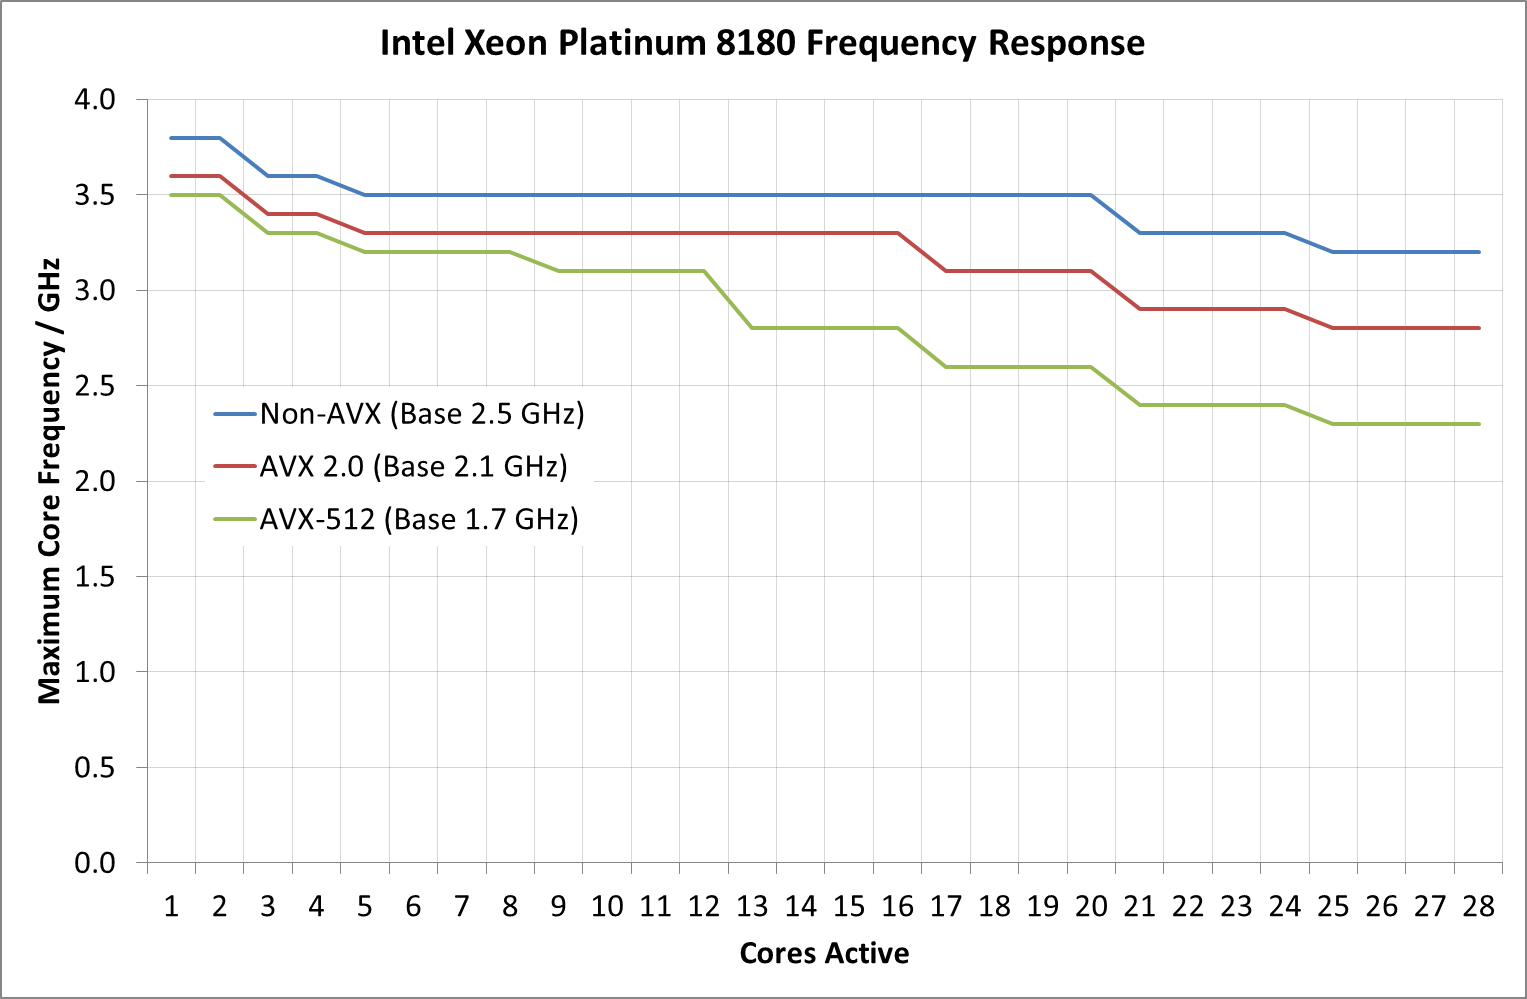
\includegraphics[width=10cm]{images/cpu_freq_avx.png}
            \caption{\label{fig:cpu_freq_avx} La fréquence soutenable par le processeur (axe des ordonnées) varie en fonction du nombre de coeur utilisés (axes des abscisses) et du type d'instructions exécutées: scalaire (en bleu), AVX 2.0 (en rouge) ou AVX 512 (en vert)\protect\footnotemark.}
        \end{figure}
        \footnotetext{Source du graphique: 
        \href{https://www.anandtech.com/show/11544/intel-skylake-ep-vs-amd-epyc-7000-cpu-battle-of-the-decade/8}{\nolinkurl{https://www.anandtech.com/show/11544/intel-skylake-ep-vs-amd-epyc}}
        }
        
        
        L'instruction \verb|rdtsc| est utilisée pour lire le compteur matériel mesurant le nombre de \textit{tics} de l'horloge depuis la dernière réinitialisation du processeur \cite{code:rdtsc}. La fréquence à laquelle ce compteur est incrémenté ne varie pas et correspond à la \textit{fréquence de base nominale} du processeur. Cette fréquence est indépendante de la fréquence d'horloge réelle, qui peut varier. Si les fréquences des processeurs devaient varier, les mesures effectuées avec \verb|rdtsc| seraient erronées. C'est pourquoi nous conseillons de fixer la fréquence du processeur avant l'exécution du micro-benchmark. Dans le cas d'une fréquence fixe différente de la fréquence de base nominale, nous avons mis en place une vérification qui calculera ensuite cette fréquence, et ajustera les résultats mesurés par \verb|rdtsc| comme le calcul de l'\gls{IPC}. Cette fonctionnalité de vérification de la fréquence et de la correction de résultat est utilisable avec l'option \verb|-F true|. Afin d'apporter les corrections voulues, nous avons besoin de mesurer la fréquence de base du processeur ainsi que la fréquence utilisée pour l'exécution.
        
        \paragraph{Mesurer la fréquence de base.} Nous avons développé un code permettant de mesurer la fréquence de base. Il utilise la fonction \verb=sleep()= qui attend un certain nombre de microsecondes ainsi que l'instruction \verb|rdtsc|. Ainsi nous pouvons calculer la fréquence avec le rapport $cycleSpent / timeSpent$ comme indiqué sur \autoref{code:base_freq}. 
        

\begin{minipage}{0.97\linewidth}         \begin{lstlisting}[label=code:base_freq ,language=C, caption={Code utilisé pour mesurer la fréquence de base du processeur. La fonction \texttt{mygettime()} utilise la fonction \texttt{gettimeofday()}\protect\footnotemark ~permet de mesurer le temps nécessaire à l'exécution du code.}]
timeStart = mygettime();
cycleInStart = rdtsc();
    usleep(10000);
cycleInEnd = rdtsc();
timeEnd = mygettime();
cycleSpent = (cycleInEnd - cycleInStart);
freq_Base = cycleSpent / (1000000000 * (timeEnd - timeStart));
\end{lstlisting} \end{minipage}
\footnotetext{gettimeofday(2) - \url{http://man7.org/linux/man-pages/man2/gettimeofday.2.html}}

        \paragraph{Mesurer la fréquence réelle.} Pour pouvoir ajuster les résultats affichés par le benchmark, il est nécessaire de connaître la fréquence à laquelle le processeur est capable d'aller. Cette fréquence peut varier en fonction de l'utilisation du mode \textit{turbo} ou si la fréquence a été limitée de façon logicielle. Pour réaliser cette mesure, nous sommes partis du constat que tous les processeurs modernes sont capables d'exécuter une soustraction sur un registre par cycle d'horloge. 
        
         
\begin{minipage}{0.97\linewidth}         \begin{lstlisting}[label=code:cur_freq ,language=C, caption={Code utilisé pour mesurer la fréquence réelle du processeur.}]
cycleInStart = rdtsc();
__asm__ ("aloop: "
    "sub $0x1,%%eax;"
    "sub $0x1,%%eax;"
    "sub $0x1,%%eax;"
    "sub $0x1,%%eax;"
    "jnz aloop" : : "a" (80000000UL)
);
cycleInEnd = rdtsc();
cycleSpent = (cycleInEnd - cycleInStart);
\end{lstlisting} \end{minipage}  
        
        Dans l'\autoref{code:cur_freq}, le registre \verb|%eax| est initialisé à \verb|80000000|. Grâce à notre hypothèse, il est possible de prévoir que le processeur réalisera ces \verb|80000000| soustractions en autant de cycles. Nous mesurons le nombre de cycles nécessaire à l'exécution du code à l'aide de l'instruction \verb=rdtsc=. Ce nombre correspond au nombre de cycle à la fréquence nominale du processeur. En faisant le rapport entre le nombre de cycles mesurés et celui attendu grâce à notre hypothèse, il est possible de déterminer si le processeur utilise une fréquence plus ou moins rapide que sa fréquence nominale. Nous calculons ainsi l'IPC de cette boucle en faisant le rapport $\frac{80000000}{cycleSpent}$.
        \begin{itemize}
            \item \verb|IPC == 1|: Le processeur utilise sa fréquence de base
            \item \verb|IPC < 1|: Le processeur utilise une fréquence inférieur à sa fréquence de base.
            \item \verb|IPC > 1|: Le processeur est capable d'exécuter des instructions à une fréquence plus élevée que sa fréquence de base (turbo).
        \end{itemize}
    
    
    
        \paragraph{Ajuster les résultats.} En connaissant la fréquence de base et la fréquence accessible par le processeur les résultats donnés par le benchmark peuvent être ajustés. Nous avons utilisé un script externe pour verrouiller la fréquence du processeur Intel Xeon 6150 à 2.00 GHz. Ce processeur a une fréquence de base de 2.70GHz. Le code présenté ci dessus nous a permis de mesurer un \gls{IPC} égale à 0.742. Cela signifie que le processeur utilise une fréquence égale à 74,2\% de sa fréquence de base, soit 2,00 GHz. Ce dernier test nous a permis de valider la méthodologie basée sur \verb|rdtsc| pour mesurer la fréquence réelle du processeur. Ainsi, nous pouvons ajuster les résultats donnés par notre outil grâce à l'option \verb|--frequency true|.

    
\subsection{Résultats}
%%%%%%%%%%%%%%%%%%%%%%%%%%%%%%%%%%%%%%%%%%%%%%%%%%%%%
    À la suite du développement du générateur de \glspl{kernel}, plusieurs expérimentations ont pu être réalisées. Dans cette section, nous présentons les principaux résultats obtenus lors de la caractérisation de processeurs Intel Skylake.
   
   
   

    \subsubsection{Vérifier les performances théoriques}
    %%%%%%%%%%%%%%%%%%%%%%%%%%%%%%%%%%%%%%%%%%%%%%%%%%%%%
    Le générateur de kernels peut être utilisé pour mesurer les performances maximales atteignables par un processeur. Cette performance mesurée en \gls{FLOPS} est notée \gls{flopspeak}. Pour illustrer cette utilisation, nous avons étudié les performances du processeur Intel Xeon 6150 cadencé à 2.7 GHz, possédant 18 coeurs et disposant d'un mode Turbo. Les résultats de cette expérimentation sont donnés dans le \autoref{tab:kg_vs_intel}. 
    
    Comme expliqué dans l'introduction ci-dessus, la fréquence  soutenable par un processeur dépend de la complexité des instructions exécutée et du nombre de coeurs utilisés. La performance de calcul théorique varie donc en fonction de chaque configuration \texttt{\{nombre de coeurs, type d'instructions, Turbo ON/OFF\}}. Pour permettre le calcul de \gls{flopspeak}, Intel donne dans sa documentation les différentes fréquences supportées par le processeur\footnote{\url{https://www.intel.com/content/dam/www/public/us/en/documents/specification-updates/xeon-scalable-spec-update.pdf}}. Ces valeurs sont reportées dans la 4e ligne du \autoref{tab:kg_vs_intel}. Pour un type d'instruction et un nombre de coeur donné, la performance du processeur dépend de l'activation ou non du turbo:
    \begin{itemize}
        
        
        \item \textbf{Turbo ON}: si le turbo est activé, la documentation du processeur donne la fréquence maximale atteignable par le processeur pour une configuration \texttt{\{nombre de coeurs, type d'instructions\}} donnée. Cette fréquence, appelée \textit{Maximum Core Frequency} (MCF), n'est pas garantie. Elle est seulement atteignable si la température du processeur le permet. En fonction de sa qualité de fabrication (fuite de courant) et de l'efficacité de son système de refroidissement, la fréquence maximale atteignable peut varier de 20\%.
        
        \item \textbf{Turbo OFF}: si le turbo est désactivé, la documentation donne la fréquence minimale que le processeur utilisera pour exécuter les instructions. Cette fréquence, appelée \textit{Base Core Frequency} (BCF), est dite \textit{garantie}, car le processeur n'utilisera pas de fréquence inférieure à celle-ci.  La fréquence BCF peut donc être utilisée pour calculer une limite inférieure de la performance du processeur. Si la température et la conception du processeur le permettent, le processeur peut utiliser des fréquences plus élevées. Cependant, comme le turbo est désactivé, la fréquence ne pourra pas dépasser la fréquence de base du processeur (2.7 GHz dans notre exemple).
        
    \end{itemize}
    
    
    Le but de cette expérimentation est d'utiliser le générateur de kernel pour vérifier la fréquence atteignable par le processeur pour différentes configuration. La fréquence maximale atteignable par le processeur n'étant pas garantie (même lorsque le turbo est activé), seul l'exécution du kernel peut permettre de mesurer la performance maximale atteignable par le processeur. Cette performance, mesurée en \gls{FLOPS}, est notée \gls{flopsmax}. Pour chaque type d'instructions (Non-AVX, AVX 2.0 et AVX-512), \gls{flopsmax} peut être mesurée en exécutant des instructions \gls{FMA}. Nous avons utilisé le générateur de kernel pour créer trois benchmarks utilisant trois tailles d'instructions (scalaire, 256 et 512 bits) avec la commande suivante:\\
\begin{minipage}{0.97\linewidth}         \begin{lstlisting}
./kg -W {64,256, 512} -O ffffffffffffff -P double -U 80 -S 1 -L 90000000
\end{lstlisting} \end{minipage}\\


    
    

    \begin{table}[h!]
    \centering
    \resizebox{\textwidth}{!}{%
    \begin{tabular}{|l|cc|cc|cc|cc|cc|cc|}
    \hline
    Jeu d'instruction & \multicolumn{4}{c|}{\cellcolor[HTML]{67FD9A}Non-AVX} & \multicolumn{4}{c|}{\cellcolor[HTML]{34FF34}AVX 2.0} & \multicolumn{4}{c|}{\cellcolor[HTML]{009901}AVX 512} \\ \hline
    Turbo & \multicolumn{2}{c|}{\cellcolor[HTML]{FFFFC7}OFF} & \multicolumn{2}{c|}{\cellcolor[HTML]{FCFF2F}ON} & \multicolumn{2}{c|}{\cellcolor[HTML]{FFFFC7}OFF} & \multicolumn{2}{c|}{\cellcolor[HTML]{FCFF2F}ON} & \multicolumn{2}{c|}{\cellcolor[HTML]{FFFFC7}OFF} & \multicolumn{2}{c|}{\cellcolor[HTML]{FCFF2F}ON} \\ \hline
    Nombre de coeurs & \multicolumn{1}{c|}{\cellcolor[HTML]{ECF4FF}1} & \cellcolor[HTML]{CBCEFB}18 & \multicolumn{1}{c|}{\cellcolor[HTML]{ECF4FF}1} & \cellcolor[HTML]{CBCEFB}18 & \multicolumn{1}{c|}{\cellcolor[HTML]{ECF4FF}1} & \cellcolor[HTML]{CBCEFB}18 & \multicolumn{1}{c|}{\cellcolor[HTML]{ECF4FF}1} & \cellcolor[HTML]{CBCEFB}18 & \multicolumn{1}{c|}{\cellcolor[HTML]{ECF4FF}1} & \cellcolor[HTML]{CBCEFB}18 & \multicolumn{1}{c|}{\cellcolor[HTML]{ECF4FF}1} & \cellcolor[HTML]{CBCEFB}18 \\ \hline
    \rowcolor[HTML]{EFEFEF} 
    Fréquence (GHz) (source Intel) & 2.7 & 2.7 & 3.7 & 3.4 & 2.3 & 2.3 & 3.6 & 3.0 & 1.9 & 1.9 & 3.5 & 2.5 \\ \cline{1-1}
    \rowcolor[HTML]{EFEFEF} 
    \gls{flopspeak} (GFLOPS) & 10.8 & 194.4 & 14.8 & 244.8 & 36.8 & 662.4 & 57.6 & 864 & 60.8 & 1094 & 112 & 1440 \\ \hline
    \rowcolor[HTML]{FFE4E2} 
    \gls{flopsmax} (GFLOPS) & 10.8 & 192.6 & 14.8 & 244.2 & 43 & 772.2 & 57.3 & 858.8 & 86 & 1430 & 112 & 1430 \\ \cline{1-1} 
    \rowcolor[HTML]{FFE4E2} 
    Fréquence calculée (GHz) & 2.7 & 2.7 & 3.7 & 3.4 & {\color[HTML]{00009B} \textbf{2.68}} & {\color[HTML]{00009B} \textbf{2.68}} & 3.58 & {\color[HTML]{000000} 2.97} & {\color[HTML]{00009B} \textbf{2.68}} & {\color[HTML]{00009B} \textbf{2.48}} & 3.5 & 2.48 \\ \hline
    \end{tabular}%
    }
            \caption{
            Mesure de la performance du processeur Intel 6150 utilisant trois jeux d'instructions (teintes vertes), avec et sans Turbo (teintes jaunes) et en utilisant un seul ou tous les coeurs (teintes violettes). Les données mesurées (en rouge) sont à comparer avec les spécifications techniques données par le constructeur (en gris). Les performances mesurées peuvent être supérieures aux performances théoriques (\gls{flopsmax} > \gls{flopspeak}) lorsque le processeur est capable de soutenir une fréquence plus élevée (en bleu) que celle annoncée par le constructeur.}
            \label{tab:kg_vs_intel}
    \end{table}
    
    

    
    La documentation du fabricant indique que le processeur étudié est capable d'exécuter deux instructions par cycle, quelle que soit la taille des instructions utilisées. Ces instructions nécessitant plus ou moins de transistors pour être exécutées (taille, nombre de coeur) le processeur doit adapter sa fréquence pour ne pas surchauffer.  Le Kernel Generator mesure le nombre d'instructions par cycle, ce qui nous permet de vérifier que deux instructions \gls{FMA} sont bien exécutées chaque cycle. Le benchmark permet de vérifier un \gls{IPC} de 2 et mesure la performance \gls{flopsmax} en GFLOPS du code. Grâce à ces deux informations, il est possible de calculer la fréquence réelle qu'utilise le processeur (dernière ligne du  \autoref{tab:kg_vs_intel}). Le calcul de la performance maximale théorique utilisant la fréquence garantie par Intel, il est possible d'obtenir \gls{flopsmax} supérieur à \gls{flopspeak}. Nous remarquons ainsi, quatre fréquences supérieures à celles annoncées par la documentation (en bleu dans le \autoref{tab:kg_vs_intel}). En effet, Intel communique la fréquence minimale garantie pour chaque configuration texttt{\{nombre de coeurs, type d'instructions, Turbo ON/OFF\}}. Cette fréquence minimale est garantie pour tous les processeurs d'un même modèle (même SKU). La qualité de fabrication du processeur peut lui permettre d'atteindre des fréquences plus élevées que celle-ci, comme indiqué en bleu dans le \autoref{tab:kg_vs_intel}. Pour étudier l'évolution de la fréquence et de la température du processeur, nous utilisons un outil développé en interne par HPE. La \autoref{pic_kg_freq_vs_temp} montre que le processeur est capable d'utiliser une fréquence de 2.7 GHz, alors que la fréquence minimale garantie est de 2.3 GHz. Le benchmark a été exécuté pendant trente minutes. Le bon système de refroidissement utilisé empêche le processeur de dépasser sa puissance TDP (Thermal Design Power) et conserve cette fréquence durant toute l'exécution. La puissance TDP est mesurée en watt et exprime la quantité de chaleur dégagée par le processeur lorsqu'il est en charge. Le TDP permet au constructeur de systèmes de refroidissement de calibrer le matériel nécessaire pour refroidir un processeur.  
    
           
    \begin{figure}[!h]
        \centering
        \begin{subfigure}[t]{0.45\linewidth}
            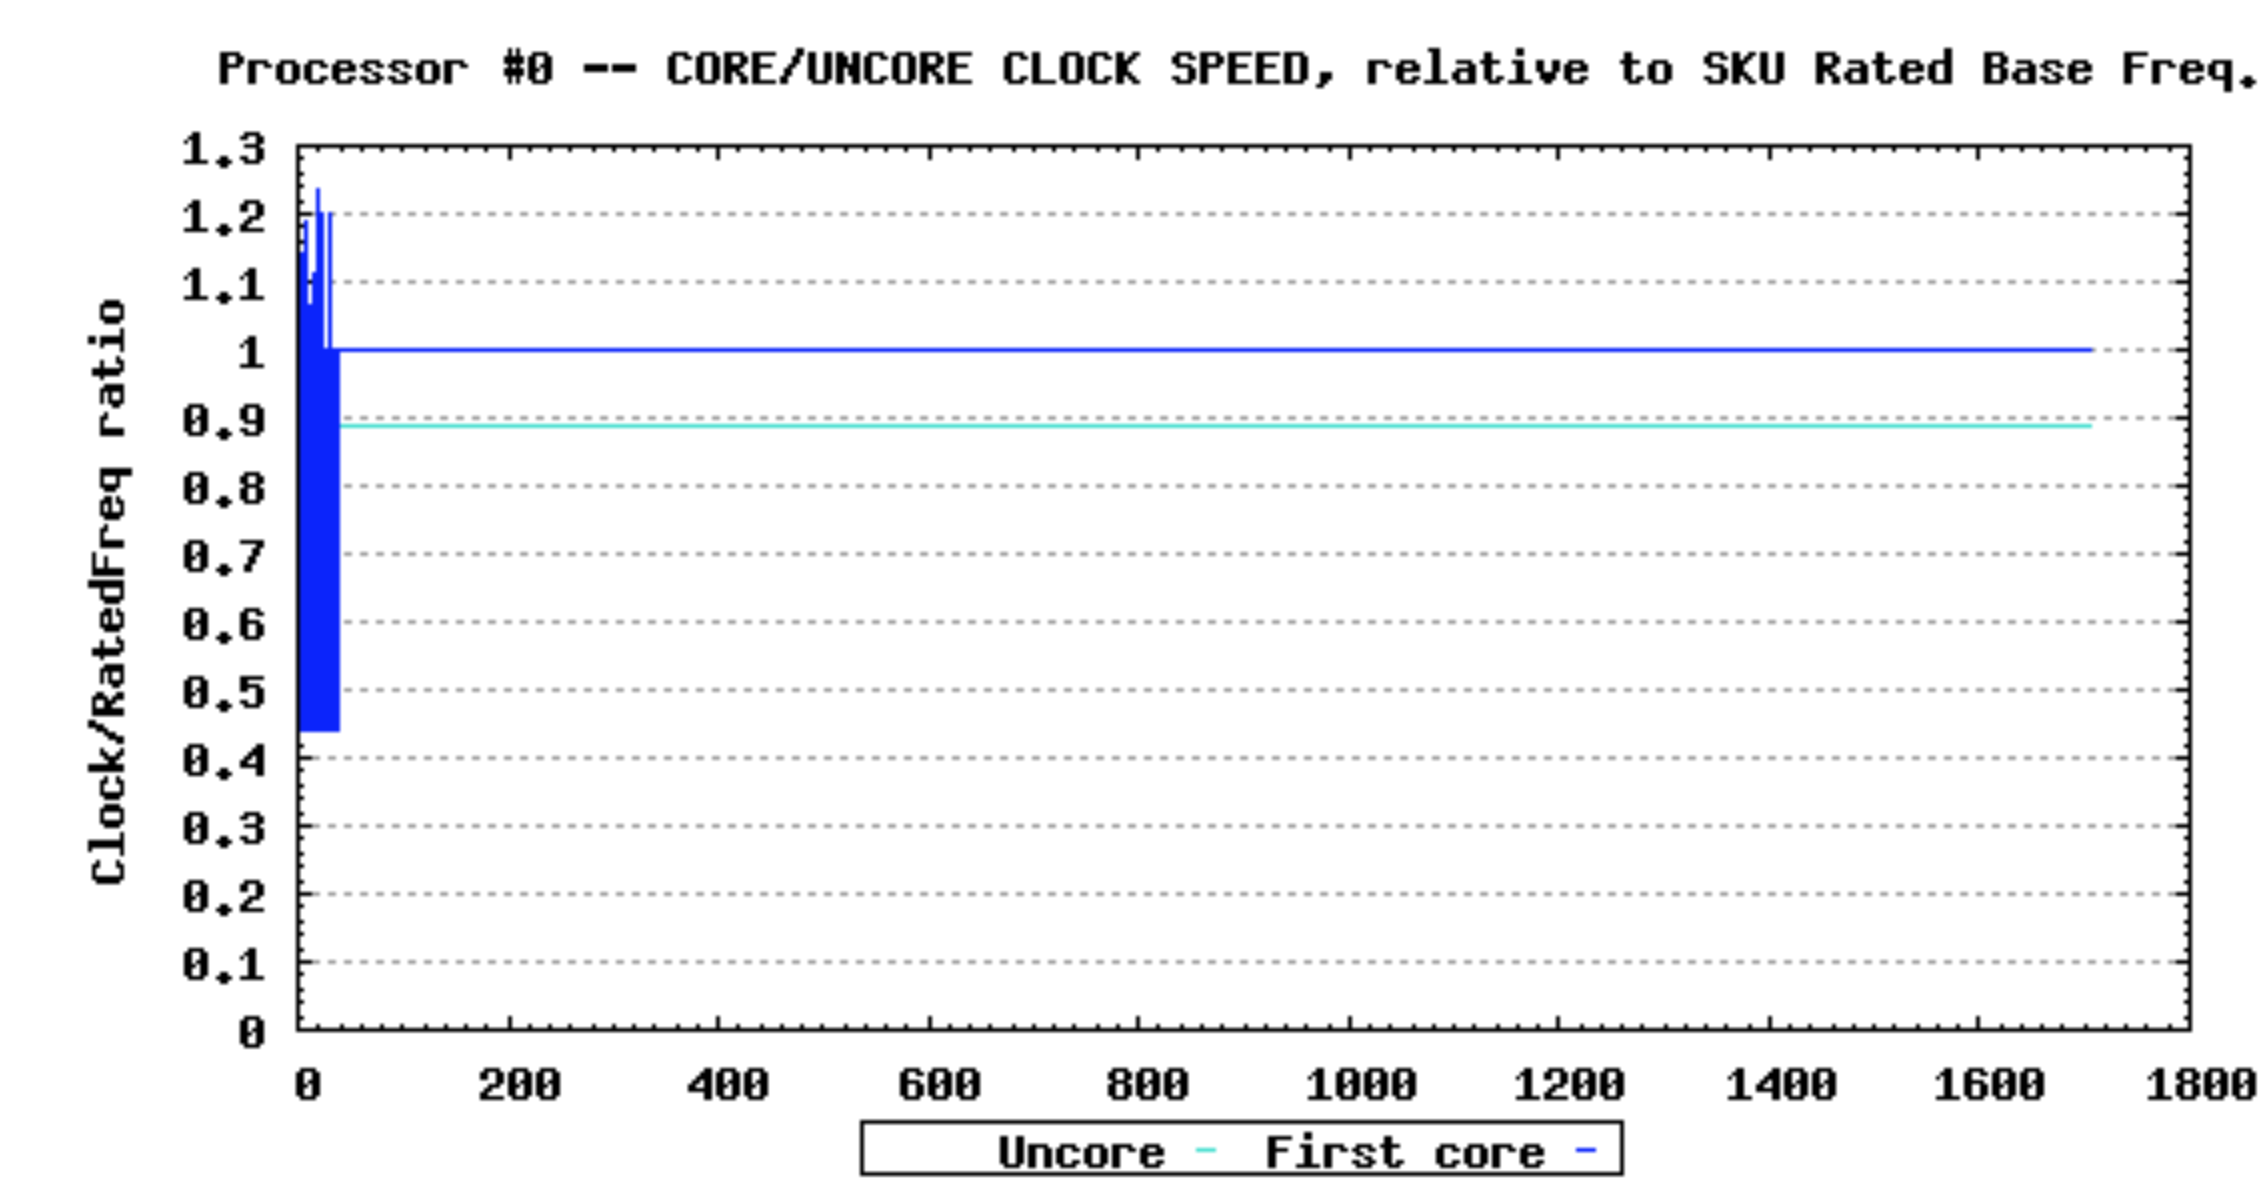
\includegraphics[width=\linewidth]{images/kg_freq.png}
            \caption{Évolution de la fréquence. Un ratio de 1 correspond à la fréquence de base de processeur (2.7 GHz).}
            \label{pic_kg_freq}
        \end{subfigure}
        ~ %add desired spacing between images, e. g. ~, \quad, \qquad, \hfill etc. 
          %(or a blank line to force the subfigure onto a new line)
        \begin{subfigure}[t]{0.45\linewidth}
            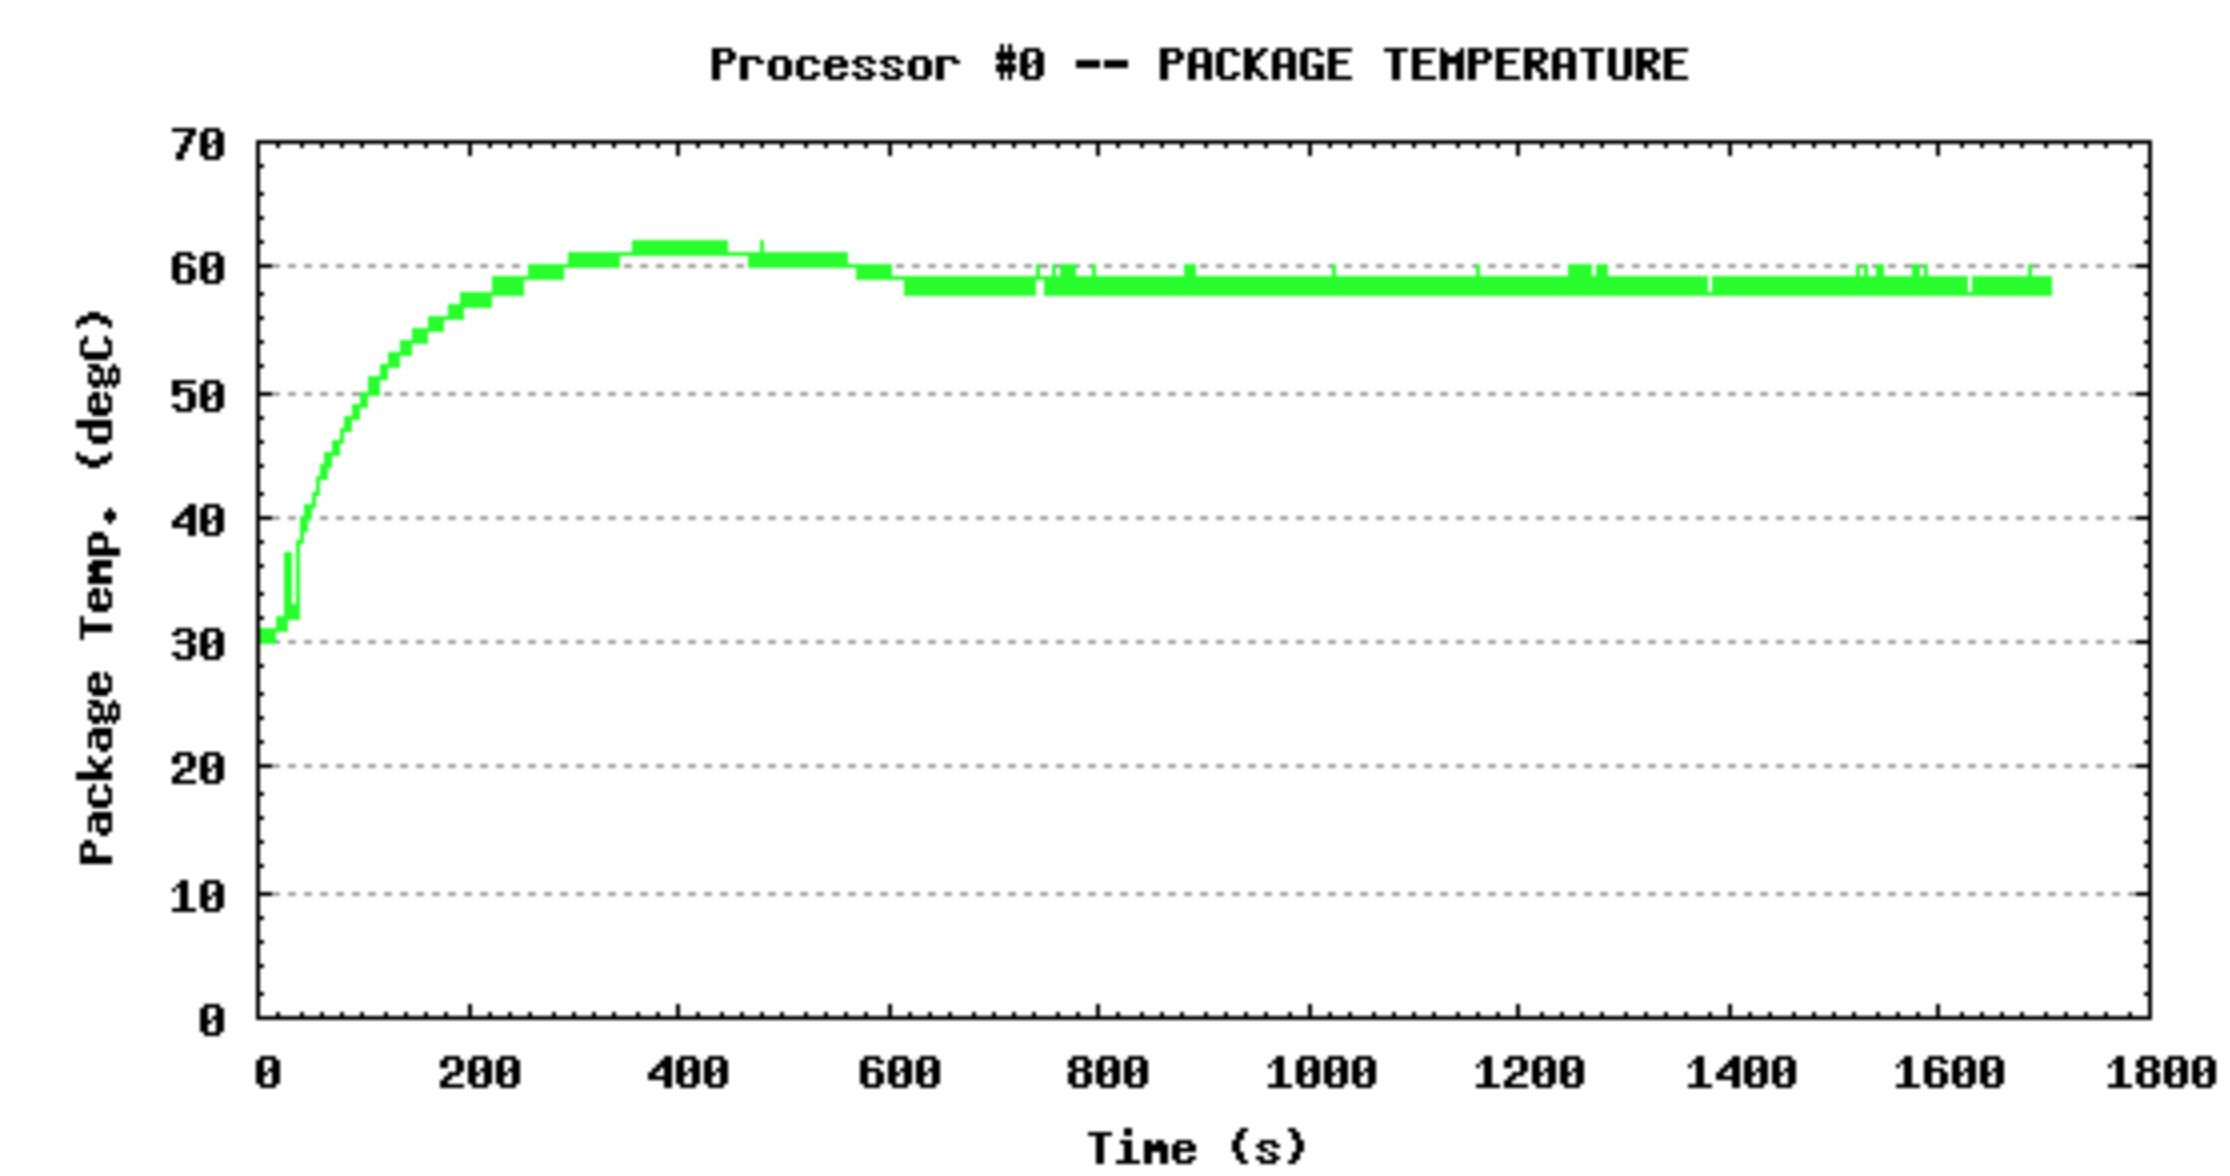
\includegraphics[width=\linewidth]{images/kg_temp.png}
            \caption{Évolution de la température du processeur}
            \label{pic_kg_temp}
        \end{subfigure}
        \caption{Évolution de la fréquence et de la température du processeur pour un benchmark AVX 2.0 exécuté sur 18 coeurs avec le turbo désactivé}\label{pic_kg_freq_vs_temp}
    \end{figure}

        




    
    \subsubsection{Caractérisation de la micro-architecture Haswell}
    %%%%%%%%%%%%%%%%%%%%%%%%%%%%%%%%%%%%%%%%%%%%%%%%%%%%%
    Lors de l'utilisation d'une nouvelle plateforme, l'utilisateur peut utiliser le générateur de benchmarks pour caractériser la microarchitecture et trouver ses points forts ou points faibles. Lors de l'arrivée des processeurs Intel de génération Haswell en 2013, certains codes ont connu des baisses de performances malgré l'utilisation d'une architecture plus récente. Nous avons utilisé le générateur de kernels pour caractériser les performances d'exécution des additions et des multiplications avec la commande suivante : \verb|./kg  -P double -W 64 -O mmmmm| permettant de générer le benchmark suivant:
    
    \begin{minipage}{0.97\linewidth}         \begin{lstlisting}[label=lst:kg_mul ,language=C]
for (i = 0; i < NB_lOOP; i++) {
timeStart = mygettime();
cycleInStart = rdtsc();
__asm__ ("" 
     "myBench:"  
   		"vmulsd %%xmm0, %%xmm1, %%xmm2; "
   		"vmulsd %%xmm0, %%xmm1, %%xmm3; "
   		"vmulsd %%xmm0, %%xmm1, %%xmm4; "
   		"vmulsd %%xmm0, %%xmm1, %%xmm5; "
   		"vmulsd %%xmm0, %%xmm1, %%xmm6; "
     "sub  $0x1, %%eax;"
     "jnz  myBench;"		:: "a" (NB_lOOP_IN));
cycleInEnd = rdtsc();
timeEnd = mygettime();
cycle_total += (cycleInEnd - cycleInStart);
time_total += timeEnd - timeStart;
}
\end{lstlisting} \end{minipage}
    
     La microarchitecture Haswell est capable d'exécuter deux multiplications par cycle. Cependant, l'utilisation du générateur de kernel nous a montré que le processeur n'était pas capable d'exécuter des additions au même rythme que les multiplications. Les résultats présentés dans le \autoref{tab:mul_vs_add} montrent que la microarchitecture Haswell est capable d'exécuter deux multiplications contre une seule addition par cycle.

    \begin{table}[h!]
    \centering
    \begin{tabular}{|l|c|c|c|c|}
        \hline
        Opération & Nombre d'instructions & Frequence & Temps & IPC \\ \hline
        Multiplication & 40000000000 & 2.1 & 7.71 & \textbf{2} \\ \hline
        Addition & 40000000000 & 2.1 & 14.43 & {\color[HTML]{963400} \textbf{1}} \\ \hline
        \end{tabular}%
        
        \caption{Différence de performance lors de l'exécution d'addition et de multiplication sur une architecture Haswell.}
        \label{tab:mul_vs_add}
    \end{table}
    
    Bien sûr, cette caractéristique est documentée et en comptant le nombre de ports destinés aux additions, l'utilisateur du processeur aurait pu en trouver la raison. Cependant la lecture de la documentation de la microarchitecture dépasse le millier de pages et en comprendre les moindres détails est plus difficile que d'utiliser les bons outils. Nous pensons que le générateur de benchmarks peut permettre à n'importe quel utilisateur de rapidement trouver ce genre de caractéristiques. Avant même d'avoir exécuté son application sur une nouvelle plateforme, il peut rapidement se faire une idée de ses performances et trouver ce genre de défauts.




    \subsubsection{Caractérisation de l'exécution dans le désordre}\label{sec:kg_out_of_order_dependency}
    %%%%%%%%%%%%%%%%%%%%%%%%%%%%%%%%%%%%%%%%%%%%%%%%%%%%%

    La puissance d'un supercalculateur vient de sa capacité à réaliser des calculs en parallèle. Pour satisfaire la loi d'Amdahl (voir \autoref{sec:amdhal}). La tâche des développeurs est de maximiser les zones de codes pouvant profiter des ressources parallèles des architectures. Le principal frein à l'utilisation du parallélisme vient de zones de codes dites séquentiels dont les instructions doivent être exécutées à la suite les unes des autres. Cela peut être dû à la dépendance d'une instruction au résultat de l'instruction précédente. Les performances d'un tel code sont souvent très mauvaises car une seule ressource de calcul (un coeur) peut être utilisée pour leur exécution. Cependant, la nature des algorithmes peut assez fréquemment laisser place à certaines optimisations. Dans le domaine des finances, les algorithmes de Monte-Carlo sont très utilisés. Ces codes ont la particularité d'exposer de longues chaînes de dépendances. En restructurant le code, le programmeur peut espérer profiter de l'exécution dans le désordre (voir \aref{sec:out_of_order}). Cela nécessite cependant d'apporter suffisamment d'instructions indépendantes au processeur pour qu'il puisse les exécuter en parallèle. Le processeur est capable d'exécuter plusieurs chaînes indépendantes les unes des autres. La performance d'une telle plateforme dépend alors de sa capacité à en exécuter plusieurs en parallèle. Grâce à l'option \verb|--dependency N| du générateur de kernels, le benchmark peut être utilisé pour caractériser cette fonctionnalité matérielle en générant $N$ chaînes indépendantes. En utilisant une dépendance de 1, chaque instruction a besoin du résultat de l'instruction précédente (voir \autoref{lst_dep1}). Dans ce cas-là, aucune parallélisation n'est possible pour le processeur. L'exécution de ce code atteint un \gls{IPC} de 0.25. Le processeur a besoin de 4 cycles d'horloge pour exécuter une instruction. Le faible IPC vient de la nécessité d'attendre que le résultat de l'opération précédente soit disponible pour pouvoir commencer à être exécutée. Sur le processeur utilisé, l'exécution d'une multiplication AVX-512 est de 4 cycles.
    
    
    
    
\begin{minipage}{0.97\linewidth}         \begin{lstlisting}[label=lst_dep1,language=C, caption=Code généré par la commande \texttt{/kg -W 512 -P double -O mmmmm -D 1}. Chaque instruction utilise le résultat produit par l'instruction précédente.]
"myBench: " 
	"vmulpd %%zmm0, %%zmm6, %%zmm2; "
	"vmulpd %%zmm0, %%zmm2, %%zmm3; "
	"vmulpd %%zmm0, %%zmm3, %%zmm4; "
	"vmulpd %%zmm0, %%zmm4, %%zmm5; "
	"vmulpd %%zmm0, %%zmm5, %%zmm6; "
"sub  $0x1, %%eax;"
"jnz  myBench;"
\end{lstlisting} \end{minipage}

     
    Pour évaluer la capacité du processeur à exécuté plusieurs chaînes indépendantes, différents nombres de chaînes ont pu être générées grâce à l'option \verb|--dependecy N|. Le code généré pour 4 chaînes est présenté sur la \autoref{pic_kg_dep_4}. En faisant varier le nombre de chaînes indépendantes, les résultats présentés dans le \autoref{tab_kg_depth} ont été obtenus. Grâce au tampon d'instructions de système d'exécution dans le désordre, le processeur est capable de commencer l'exécution de plusieurs chaînes indépendantes simultanément. Nous avons pu valider que le processeur est capable d'exécuter au moins 8 chaînes d'instructions indépendantes. Le processeur peut exécuter une multiplication par cycle par pipeline (2 au total). La latence d'une multiplication AVX-512 étant de 4 cycles, le processeur a besoin de 8 chaînes indépendantes pour utiliser la totalité de la puissance du processeur. Cette caractéristique du processeur doit être connue par le programmeur pour transformer son code et obtenir le maximum de performance du processeur. Grâce au générateur de kernels, les nouvelles architectures peuvent être testées pour caractériser ces performances et prévoir leur performance pour des codes pouvant utiliser des chaînes de calculs indépendantes comme la résolution de polynômes par exemple. 
    
         \begin{figure}
            \center
            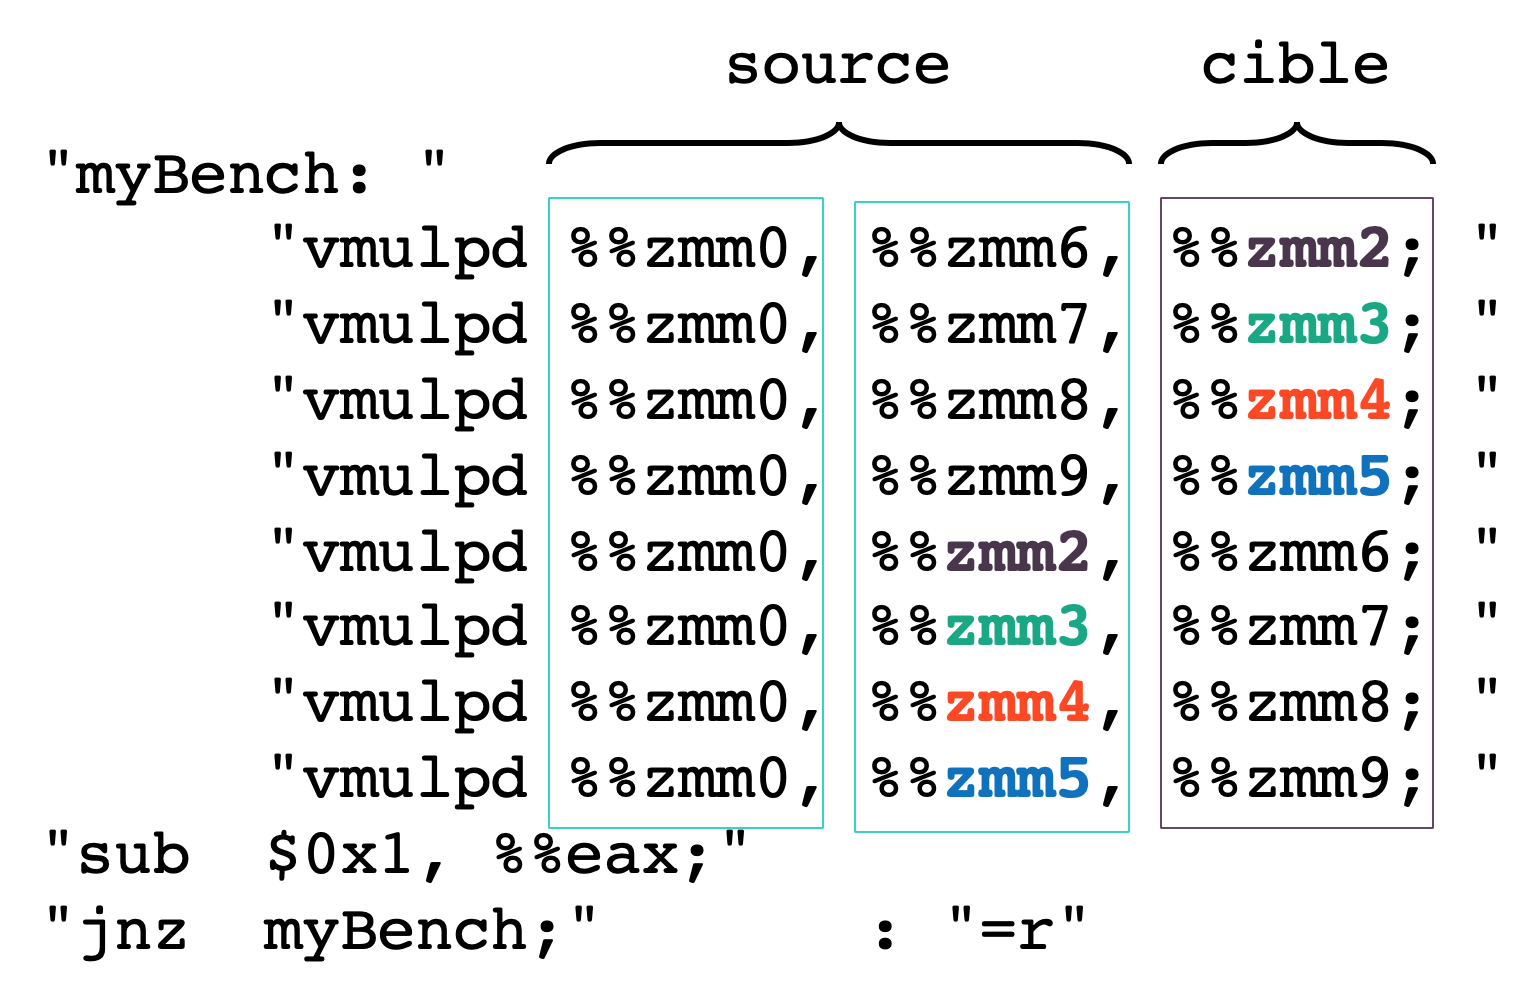
\includegraphics[width=8cm]{images/kg_dep_4.png}
            \caption{\label{pic_kg_dep_4} Code généré par la commande \texttt{/kg -W 512 -P double -O mmmmmmmm -D 4}. Les quatre chaînes de dépendances sont représentées par les quatre couleurs utilisées.}
        \end{figure}

    \begin{table}[h!]
    \centering
    \normalsize
    \begin{tabular}{|l|c|c|c|c|c|c|c|c|c|c|}
    \hline
    Nombre de chaînes & 1 & 2 & 3 & 4 & 5 & 6 & 7 & 8 & 9 & 10 \\ \hline
    IPC & 0.25 & 0.50 & 0.75 & 1 & 1.25 & 1.50 & 1.75 & 2 & 2 & 2 \\ \hline
    \end{tabular}%
    \caption{Mesure du nombre d'instruction par cycle pour un nombre de chaîne de dépendance $N$, dans un benchmark généré à l'aide de la commande \texttt{/kg -W 512 -P double -O mmmmmmmm -D N}. Au moins 8 chaînes d'instrutions indépendantes doivent être présentées au processeur pour l'utiliser au maximum de ses performance (IPC égal à 2).}
    \label{tab_kg_depth}
    \end{table}





    \subsubsection{Caractérisation de la FPU de deux processeurs Skylake}

        La dernière génération de processeur Intel Skylake est répartie en quatre gammes (Bronze, Silver, Gold et Platinium). Les fonctionnalités et les performances des processeurs des différentes gammes étant différentes (voir \autoref{table:skl}), il est important pour notre équipe avant-vente d'en connaître les caractéristiques et les performances pour adapter les configurations des serveurs aux demandes clients. Les processeurs des gammes Bronze ou Silver sont rarement choisis pour répondre à un appel d'offres compte tenu de leurs caractéristiques plus faibles (une FPU au lieu de deux, nombre plus faible de coeurs). Les processeurs haut de gamme (Gold et Platinium) possèdent généralement plus de coeurs, et sont capables d'utiliser des fréquences plus élevées que les processeurs d'entrée de gamme (Bronze et Silver). Bien sûr, comme ces processeurs coûtent plus cher à l'achat, un client choisira un processeur en fonction de son budget, de sa consommation électrique ou du profile de son application.
        
        
        \begin{table}[h!]
        \centering
        \resizebox{\textwidth}{!}{%
        \begin{tabular}{|l|l|l|l|l|l|}
        \hline
        \rowcolor[HTML]{EFEFEF}
        Gamme - référence CPU                                &   Bronze: 31xx                    & Silver: 41xx              & Gold: 51xx            & Gold: 61xx            & Platinium: 81xx           \\ \hline
        Nb. canaux mémoire et vitesse    & 6-ch@2133 Ghz                         & 6-ch\textbf{@2400}      & 6-ch@2400           & 6-ch\textbf{@2666}   & 6-ch@2666                \\ \hline
        Lien UPI (scalabilité)         &     2   (2S-2UPI)       & 2  (2S-2UPI)    & 2 (4S-2UPI)  & 3  (2S-3UPI) & 3    (8S-3UPI)    \\ \hline
        Débit UPI                   & 9.6 GT/s                          & 9.6 GT/s                  & 10.4 GT/s              & 10.4 GT/s             & 10.4 GT/s                 \\ \hline
        HyperThreading  \cite{Marr2002}                &   NON                              & \textbf{OUI}              & OUI                   & OUI                   & OUI                       \\ \hline
        FMA-512 FPU                     &     1                             & 1                         & 1                     & \textbf{2 }           & 2                         \\ \hline
        
        \end{tabular}
        }
        \caption{Principales différences entre les gammes de processeurs Intel de génération Skylake.}
        \label{table:skl}
        
        \end{table}
        
      
      Pour caractériser la performance crête des processeurs \gls{flopsmax}, notre équipe de benchmark utilise des codes tels que HPL. Pour obtenir la meilleure performance atteignable, le benchmark HPL est compilé pour utiliser les instructions vectorielles les plus grandes supporté par le processeur étudié (ici des instructions AVX-512). Les résultats du benchmark Linpack donnés dans le \autoref{table:skl_bench}, montrent que les processeurs les plus performants sont ceux appartenant aux gammes Gold et Platinium. Cette différence de performance peut être expliquée par la présence de deux \gls{FPU} sur les processeurs haut de gamme. Ces deux FPU sont capables d'exécuter chacune une instruction \gls{FMA} AVX-512 par cycle. Grâce au générateur de kernel, cette caractéristique a pu être vérifiée (voir \autoref{table:skl_bench}). 

        \begin{table}[h!]
        \centering
        
        \resizebox{\textwidth}{!}{%
        \begin{tabular}{|l|l|l|l|l|}
        \hline
        \rowcolor[HTML]{EFEFEF}
        Processeur (Nb. FPU)    & Silver: 4110 (1)  & Gold: 5117 (1)   & Gold: 6130 (2)    & Platinium: 8160 (2)        \\ \hline
        Instruction AVX-512 FMA par cycle   & 1             & 1            & 2             & 2                    \\ \hline
        Benchmark HPL (GFLOPS)            & 297           & 372          & 714           & 716                  \\ \hline
        
        \end{tabular}
        }
        \caption{Pour différents processeur, le nombre d'instruction FMA AVX-512 pouvant être exécutée chaque cycle a été mesuré à l'aide du \texttt{Kernel Generator}. En fonction du nombre de FPU présent sur un coeur (1 ou 2), le nombre d'instructions exécuté varie (1 ou 2). La performance \gls{flopsmax} du benchmark HPL mesurée GFLOPS varie de la même façon suivant la gamme du processeur utilisé. Afin de pouvoir comparer les différentes gammes de processeurs la configuration suivante à été appliqué à chaque processeur: désactivation de l'\textit{hyperthreading}, fréquence limitée à 1.5 GHz, utilisation de 8 coeurs. \textbf{todo: revoir les valeurs}}
        \label{table:skl_bench}
        \end{table}
        % 1 FPU : 8 * 2 *1 *1.5 * 8 = 192
        % 2 FPU : 8 * 2 *2 *1.5 * 8 = 384
        
        
        Afin d'estimer l'impact d'une FPU manquante sur la performance d'une application réelle, nous avons utilisé une application de CFD typique. L'application utilisée n'exécute que des instructions vectorielles de 256 bits (AVX-2). Nous nous attendons alors à obtenir des performances différentes entre un processeur Silver et Gold pour une application qui n'est pas limitée par la bande passante mémoire. Étonnamment, les résultats obtenus sur ces deux plateformes sont très proches. Pourtant, nous avons bien montré que les processeurs de gamme supérieure possèdent une FPU de plus et sont donc deux fois plus performants. Pour comprendre ce phénomène, nous avons utilisé le générateur de benchmark pour générer un kernel de calculs utilisant des instructions vectorielles de 256 bits. La performance mesurée pour le kernel sont reportés dans le \autoref{table:skl_bench2}.  
        
       
        
        
        \begin{table}[h!]
        \centering
        % increase table row spacing, adjust to taste
        %\renewcommand{\arraystretch}{1.1}
        % COMMENTS if using array.sty, it might be a good idea to tweak the value of
        %\extrarowheight{1} as needed to properly center the text within the cells

        \resizebox{0.4\textwidth}{!}{%
        \begin{tabular}{|l|l|l|l|l|}
        \hline
        \rowcolor[HTML]{EFEFEF}
                                & Silver: 4110       & Gold: 6130      \\ \hline
        IPC                     & 2                  & 2           \\ \hline
        GFLOP/s                 & 2.38e+10           & 2.37e+10           \\ \hline
        \end{tabular}
        }
        \caption{Mesure de la performance de processeur de deux gammes différentes à l'aide du \texttt{Kernel Generator} et de la commange suivante: \texttt{/kg  -P double -W 256 -O ffffffff}. Alors que le processeur de la gamme Gold possède une FPU de plus, il obtient des performances similaires à celles du processeur de gamme Silver.}
        \label{table:skl_bench2}
        \end{table}
        
        Bien que le processeur Intel Xeon Silver 4110 ne possède qu'une seule FPU, il est capable d'exécuter deux instructions AVX-2 par cycle. Cette caractéristique peut être retrouvée dans la documentation du processeur \footnote{source: \url{https://en.wikichip.org/wiki/intel/microarchitectures/skylake\#Execution_engine_2}}. Les FPU des processeurs Skylake d'entrée de gamme fusionnent deux ports de 256 bits pour former la FPU 512-bits. Cependant, lorsque des instructions de 256 bits sont exécutées, le processeur peut utiliser les deux ports indépendamment pour exécuter deux instructions de 256 bits. La FPU supplémentaire sur les processeurs haut de gamme est une FPU 512 bits qui ne permet pas d'utiliser cette caractéristique et qui pourrait permettre d'exécuter (en théorie) quatre instructions par cycle.
        Afin de mieux comprendre comment cette fusion d'instructions fonctionnait, nous avons utilisé le générateur de benchmarks pour générer des \glspl{kernel} possédant des instructions vectorielles de taille différentes. Les résultats des différentes expérimentations sont reportés dans le \autoref{res:skl}. Chaque cycle, la FPU est capable d'exécuter différentes combinaisons d'instructions: 


        \begin{itemize}
            \item Une instruction AVX 512 bits.
            \item Deux instruction AVX 256 bits.
            \item Deux instructions AVX 128 bits.
            \item Deux instructions scalaire.
            \item Toutes combinaisons de deux instructions dont la taille agrégée ne dépasse pas 512 bits.
        \end{itemize}
        
        
        \begin{table}[h!]
        \normalsize
        % increase table row spacing, adjust to taste
        %\renewcommand{\arraystretch}{1.1}
        % COMMENTS if using array.sty, it might be a good idea to tweak the value of
        %\extrarowheight{1} as needed to properly center the text within the cells
        \centering
        %\resizebox{\textwidth}{!}{%
        \begin{tabular}{|l|c|c|c|c|}
            \hline
            \rowcolor[HTML]{EFEFEF} 
            Gamme & Silver & Gold & Gold & Platinium \\ \hline
            \rowcolor[HTML]{EFEFEF} 
            Ref. processeur Intel Skylake & 4110 & 5117 & 6130 & 8160 \\ \hline
            \rowcolor[HTML]{EFEFEF} 
            Nombre de FPU & 1 & 1 & 2 & 2 \\ \hline
            128 + scalaire & \textbf{2} & \textbf{2} & 2 & 2 \\ \hline
            256 + scalaire & \textbf{2} & \textbf{2} & 2 & 2 \\ \hline
            256 + 128 & \textbf{2} & \textbf{2} & 2 & 2 \\ \hline
            256 & \textbf{2} & \textbf{2} & 2 & 2 \\ \hline
            512 + scalaire & 1 & 1 & 2 & 2 \\ \hline
            512 + 128 & 1 & 1 & 2 & 2 \\ \hline
            512 + 256 & 1 & 1 & 2 & 2 \\ \hline
        
        \end{tabular}
        %}
        \caption{Mesure du nombre d'instruction exécuté chaque cycle pour différents processeur. La FPU des processeurs d'entrée de gamme est capable de fusionner certaines instructions (en gras) pour les exécuter en un seul cycle.}
        \label{res:skl}
        \end{table}
        
        
        
       Ainsi, le processeur haut de gamme bénéficie des deux FPU lorsque le code est capable d'utiliser des instructions vectorielles de 512 bits. Il est fréquent que les applications n'y parviennent pas (mauvaise vectorisation du code, problème du compilateur, dépendances) et utilisent des instructions vectorielles plus petites, les processeurs d'entrée de gamme obtiennent des performances rigoureusement égales. Évidement, la FPU n'est pas la seule responsable de la performance d'une application, le \autoref{table:skl} montrent bien que d'autres caractéristiques diffèrent telles que le nombre de liens UPI ou la possibilité d'utiliser l'hyperthrading . Le but du générateur de kernels est de caractériser une architecture pour le besoin d'une application. Grâce au caractéristique découverte suite à cette expérimentation, plusieurs réponses à des offres d'appels ont été réalisées avec des processeurs d'entrée de gamme. Grâce à cette caractéristique, les applications utilisant des instructions AVX-2 peuvent obtenir des performances assez proches sur des processeurs coûtant beaucoup moins cher.


        
        




%    \subsubsection{Expliquer les performances d'un code}
    %%%%%%%%%%%%%%%%%%%%%%%%%%%%%%%%%%%%%%%%%%%%%%%%%%%%%
 %   Une autre utilisation du générateur de kernel peut permettre d'expliquer les performances d'une autre application. 
    
    
  %   What we have seen in the past months with the releases of the new Skylake processors is that entry level processors like Intel 4110 can perform as good as a top bin processor like the Intel 6148 for real applications thus increasing the $\frac{performance}{price}$ of a large scale cluster. 


\subsection{Conclusion}
%%%%%%%%%%%%%%%%%%%%%%%%%%%%%%%%%%%%%%%%%%%%%%%%%%%%%
    
    L'outil \verb=Kernel Generator= est un générateur de benchmarks qui permet de mesurer la performance maximale (\gls{flopsmax})  d'un processeur pour un type d'instruction vectorielle utilisant différentes configurations (type d'instructions, dépendances...).
    Le générateur de kernel assembleur est un outil très précis pour la caractérisation des \gls{FPU}. Le principal avantage de l'utilisation de l'assembleur est d'éliminer les optimisations du compilateur. Le benchmark doit assurer à l'utilisateur qu'il mesure bien la performance du code qu'il a choisi de générer et qu'il n'a pas été modifié durant la compilation. Il nous a permis d'atteindre des performances souvent égales aux performances théoriques (\gls{flopspeak}). En utilisant le générateur, le programmeur peut être amené à découvrir des particularités de la microarchitecture (comme celle de l'exécution dans le désordre). En comprenant précisément le fonctionnement de la FPU, il pourra même trouver des optimisations pour sa propre application.
    
    Pour le moment, seul l'ISA x86 est supporté, mais l'outil a été codé de façon à faciliter l'ajout d'une nouvelle ISA. Nous avons choisi de commencer à le développer pour des processeurs dont nous connaissons bien le comportement pour valider son bon fonctionnement. L'exemple de la FPU du processeur Intel Xeon 4110, nous a permis de montrer que même sur des architectures que nous connaissons bien, certaines spécificités nous échappent encore. L'utilisation du générateur permet d'en comprendre toutes les particularités.
    
    
    \paragraph{Futures travaux.} La suite du travail comprend la fin du développement de l'option permettant de mixer différentes tailles d'instructions vectorielles dans le même kernel. Nous pensons aussi permettre de générer des instructions générant des déplacements mémoires pour vérifier qu'elles ne gênent pas l'exécution des instructions de calculs. Enfin, pour mieux caractériser les plateformes pour certaines applications comme en cryptographie, nous allons ajouter d'autres instructions pouvant être générées (rotation, décalage...).
    
    \newpage
        \section{Monitoring du bus mémoire}\label{sec:yamb}


Cette section présente l'outil YAMB (\textit{Yet Another Memory Bandwidth profiling tool}). YAMB établit le profil de chaque contrôleur de mémoire en mesurant le nombre de transactions (lecture et écriture) ainsi que le nombre d'évènements \textit{miss} dans le dernier niveau de cache (LLC). Ensuite, il utilise un script python pour dessiner un graphique montrant l'évolution des trois métriques.

\begin{figure}[h!]
\center
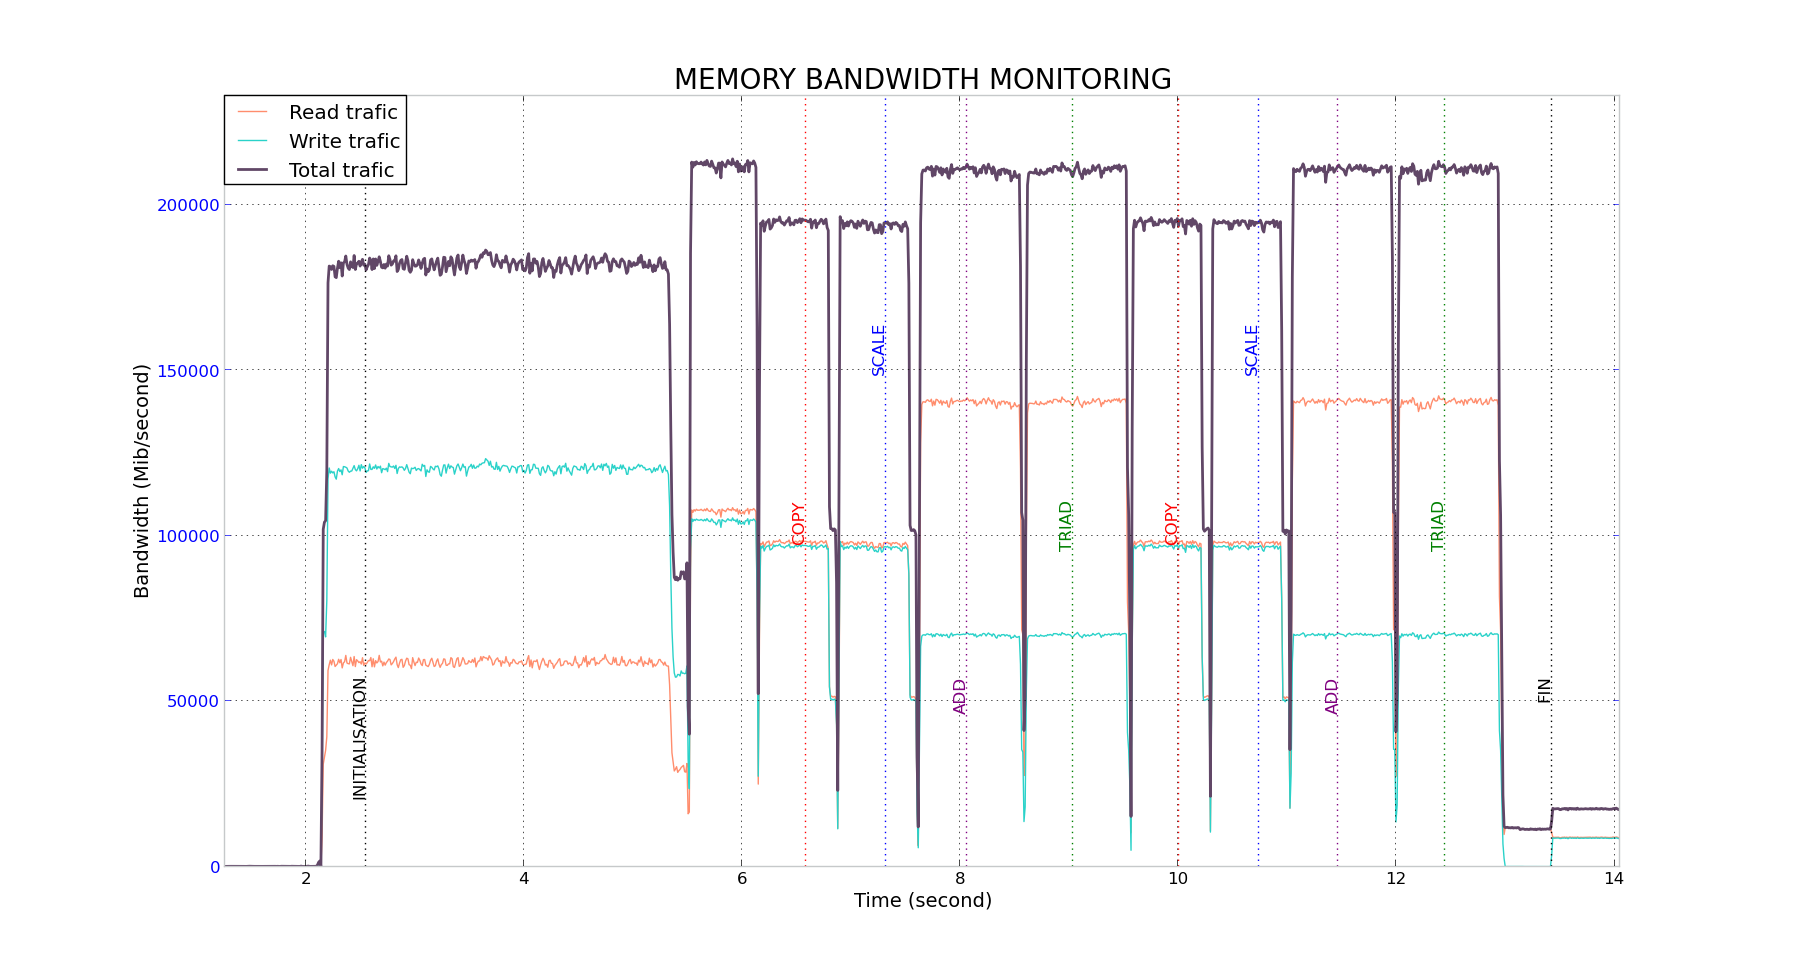
\includegraphics[width=16cm]{images/yamb_stream.png}
\caption{\label{pic:yamb_stream} Exemples d'utilisation de l'outil \texttt{YAMB} pour suivre l'activité du bus mémoire lors de l'exécution du benchmark \texttt{STREAM} pour deux itérations des 4 noyaux de calculs: \texttt{copy}, \texttt{scale}, \texttt{add} et \texttt{triadd}.}
\end{figure}




\subsection{Introduction}
%%%%%%%%%%%%%%%%%%%%%%%%%%%%%%%%%%

    \subsubsection{Motivation}
     %%%%%%%%%%%
     
        Comme présenté dans le \autoref{chap:sota:materiel}, le bus mémoire d'une architecture Von Neuman est le principal goulot d'étranglement des performances des applications de calculs intensifs\cite{Drepper2007}. Le bus mémoire est une ressource partagée par les coeurs d'un même processeur. La mauvaise utilisation de celui-ci par un coeur affecte la performance des autres. Nous observons une augmentation du nombre de coeurs sur les processeurs de dernière génération sans réelle évolution de la performance du bus mémoire. Cette disparité résulte en une augmentation d'accès concurrents à cette ressource partagée limitant la performance des applications. Il est donc primordial de s'assurer de son utilisation optimale (saturation et transferts de données utiles). Pour s'en assurer, il n'est pas possible de réaliser une mesure sur la totalité de l'application (ou d'un noyau de calculs). En effet, une application peut être limitée par la performance du bus, sans qu'il soit saturé. En effet, le déclenchement des accès mémoire par le processeur n’est pas toujours optimal pour saturer le bus mémoire sur la totalité de l'exécution. Par exemple si les accès sont tous réalisés au même moment, le bus peut être saturé pendant un court instant et être ensuite inutilisé. Sur la totalité de l'exécution, on obtiendra une mesure qui indiquera que le bus n'est pas saturé alors qu'il s'agit bien du goulot d'étranglement des performances de l'application. Le bus mémoire étant une ressource critique, il doit être utilisé pour transférer le plus possible de données utiles. Les transferts entre la mémoire et le processeur se font  par paquet (ligne de cache). Il est primordial que le maximum des données présent dans cette ligne de cache soit utilisées pour un calcul lorsque celle-ci est transférée vers le processeur. Pour cela, une adaptation des structures de données peut être nécessaire.
    
    \subsubsection{Objectifs}
    %%%%%%%%%%%
    
        L'objectif de l'outil présenté dans cette section est de répondre aux deux prérogatives indiquées dans précédemment: saturation du bus et utilisation effective. Pour y répondre, l'utilisateur doit posséder un outil lui permettant de suivre son activité avec une résolution fine (de l'ordre de la milliseconde). L'outil en question doit pouvoir distinguer les accès réalisés en lecture et en écriture pour pouvoir s'assurer de l'utilisation effective du bus. Cette méthodologie est présentée dans la section \autoref{sec:smm}.

    \subsubsection{Verrous}
    %%%%%%%%%%%
        
        
        Le système d'exploitation n'a généralement pas connaissance de l'évolution des accès mémoire, contrairement à d'autres ressources comme les I/O où le système d'exploitation réalise l'intermédiaire avec l'application. Mis à part certaines tâches comme la gestion des pages, les accès mémoire sont réalisés par le contrôleur mémoire. Comme étudié dans la \autoref{sec:edl_perf_uncore}, ces compteurs sont situés sur les PMU \textit{uncore}. Sur des architectures modernes telles que les processeurs Intel Skylake, ces compteurs comptent précisément tous les accès mémoire réalisés en distinguant la lecture et  l'écriture. Cependant, comme les compteurs ne sont associés à aucun coeur, il est impossible de faire correspondre un accès mémoire au coeur et donc au processus qui en est responsable. Notre outil a pour objectif d'analyser l'activité d'applications HPC qui utilisent généralement tous les coeurs des processeurs pour la même application. Cette particularité n'est donc pas un verrou majeur pour notre développement. Pour des outils nécessitant plus de précision \cite{Larysch2016}, l'utilisation de ces compteurs n'est cependant pas possible. Les moyens disponibles pour les programmer sont complexes et propres à chaque architecture. Le développement d'un outil utilisant une programmation directe des compteurs rend très difficile la portabilité de l'outil sur différentes architectures.
  
          
    \subsubsection{État de l'art}
    %%%%%%%%%%%%%%%%%%%%%%%%%%%%%%%
    
        Les évènements se produisant sur un processeur peuvent être comptés à l'aide de compteurs matériels. Ils sont accessibles par le biais de composants appelés Performance Monitor Units (PMU). Sur les CPU modernes, il y a au moins deux PMU : une sur le noyau et une sur le socket responsable des évènements qui s'y rapportent (comme l'accès mémoire). Ces compteurs varient d'une architecture à l'autre, ou d'un modèle de processeur à l'autre, ce qui les rend difficiles à programmer et à maintenir. Que ce soit pour le core ou le uncore, ces méthodes sont assez complexes à utiliser et à maintenir. C'est pourquoi nous utilisons des interfaces de haut niveau telles que \textit{PAPI} ou \textit{perf} qui nous permettent de ne plus dépendre de l'implémentation des compteurs à bas niveau. 
        
        De nombreux outils ont été développés pour suivre l'activité du CPU (voir \autoref{sec:edl_monitoring_tools}). Intel propose deux outils, \verb|VTune|\cite{reinders2005vtune} et Intel MBM \footnote{Intel MBM - \url{https://github.com/intel/intel-cmt-cat/wiki}}. Le premier est un outil propriétaire nécessitant une licence payante. Le deuxième est proposé en libre accès sur le dépôt en ligne d'Intel mais n'est compatible qu'avec des architectures Intel.
        
        D'autres outils tels que \verb=TAU= ou \verb=Extrae= présentent de nombreuses informations à l'utilisateur qui rendent difficile la compréhension des résultats. De plus, ce grand nombre d'informations nécessite généralement l'utilisation de plusieurs compteurs matériels qui peuvent ne plus être présents d'une architecture à l'autre. La complexité des outils peut aussi les rendre dépendants de librairies externes non compatibles avec certaines architectures rendant leur utilisation impossible (\verb|MAQAO|).
        
        L'outil \textit{Likwid} propose de mesurer les données transférées (GB) et leur débit (GB/s) pour un noyau de calcul. Il peut aussi générer des traces pour suivre plus précisément l'utilisation du bus mémoire, mais l'outil de visualisation des données n'est plus supporté.
        
        D'autres travaux tels que \textit{Memguard}\cite{Yun2013} mesurent le nombre de \textit{miss} dans le dernier niveau de cache pour en déduire le trafic du bus mémoire. Malheureusement, avec la complexification des architectures et l'utilisation constante des unités de préchargement mémoire, certains transferts mémoires sont réalisés avant qu'un évènement \textit{miss} ne soit déclenché. Il n'est donc plus possible de mesurer le trafic mémoire avec ces techniques-là. 

      
    

\subsection{Développement}
%%%%%%%%%%%%%%%%%%%%%%%%%%%%%%%%%%

    \subsubsection{Choix de l'interface}
        
            De nombreux outils et interfaces ont été développés pour accéder aux compteurs matériels avec leurs avantages et leurs inconvénients. Les principales contraintes de nos développements sont la portabilité des outils et l'accès libre aux sources. Likwid et \textit{Perf Events} sont les outils répondant au maximum des critères de développement énoncés précédemment. Cependant, l'outil de visualisation de Likwid n'est plus supporté. Pour ces raisons et afin d'éviter une surcouche supplémentaire, nous avons choisi de développer nos outils en nous basant sur le système de suivi de performance \textit{Perf Events}. En effet, son intégration dans le noyau lui assure une certaine pérennité et il permet d'utiliser des évènements natifs lorsque les noms symboliques ne sont pas supportés. Ainsi, nous nous assurons un maximum de compatibilité avec les architectures émergentes.
            
            Bien qu'il s'agisse avant tout d'un outil d'espace utilisateur, la commande perf fait partie du noyau Linux du point de vue du développement. Faire partie de Linux assure une haute exigence du développement du code ainsi qu'un support au fil des versions du noyau. Lorsque le noyau supporte le nom symbolique des évènements, \textit{perf} est très simple à utiliser. Dans le cas contraire, \textit{Perf Events} offre la possibilité aux utilisateurs expérimentés d'encoder leurs propres évènements.
            
            L'inclusion de \textit{Perf Events} au projet Linux peut aussi être un inconvénient en rendant l'outil intrinsèquement lié à la version du noyau Linux. Ceci implique que pour utiliser les nouvelles fonctionnalités de perf il faut généralement installer la version du noyau correspondante. La deuxième difficulté vient de l'appel système \textit{perf\_event\_open}. S'il permet d'éviter à l'utilisateur d'écrire manuellement les différents bits de configuration des MSR, beaucoup de travail reste à faire pour le développeur désireux de profiler ses applications. Parce que Linux supporte de nombreux processeurs différents possédant différentes versions de PMU, les développeurs de noyau ont dû laisser la charge de beaucoup de détails de microarchitecture de bas niveau dépendant du code utilisateur. En conséquence, cet appel système est très complexe à utiliser et ne peut pas être utilisé de manière portable. Les principales difficultés consistent à trouver les événements à compter ou à échantillonner, à configurer tous les paramètres à transmettre à l'appel système et à effectuer plusieurs appels système en fonction du nombre de \textit{threads} de l'application profilée et du nombre de coeurs utilisés. Ces différentes difficultés (programmation, portabilité) ont été les principales motivations du développement d'autres outils tels que PAPI, Intel Performance Counter Monitor (PCM) ou NUMAP\cite{Selva2017}.

    \subsubsection{Perf Events}
    %%%%%%%%%%%%%%%%%%%%%%%%
     
        YAMB est plus un utilitaire pour la commande \textit{perf} qu'un outil autonome. Comme présenté dans \autoref{sec:edl_profiling_perf}, \textit{perf} est l'outil de profilage de Linux, et nous espérons que sa large disponibilité le rendra facilement utilisable par le plus grand nombre de personnes.  En raison des permissions limitées que les utilisateurs ont sur les clusters l'outil doit utiliser une interface ne nécessitant pas de droits privilégiés (\textit{root}) pour y accéder. Du fait du développement de l'interface \verb=perf_event= dans le code noyau il est possible pour l'administrateur d'autoriser les utilisateurs normaux à accéder aux compteurs. Cela peut être fait en écrivant la valeur 1 dans le fichier \verb=/proc/sys/kernel/perf_event_paranoid=.
        
        La commande \verb=perf= peut être utilisée pour programmer les PMU \textit{uncore} et accéder aux compteurs des contrôleurs mémoires. L'outil YAMB utilise cette commande pour configurer les PMU pour qu'elles comptent les transactions en cours sur chaque canal mémoire, en lecture et en écriture. La commande peut aussi être utilisée pour compter le nombre d'évènements \textit{miss} dans le cache de dernier niveau (optionnel).
        
        Le coeur de l'outil de profilage YAMB est le lancement de la commande \verb=perf= en arrière-plan et le traitement des données dans un fichier de sortie. Ensuite, un script peut être utilisé pour dessiner le graphique. 
        L'outil \verb=YAMB= reçoit deux options \verb=--start= et \verb=--stop=. L'utilisation de la première option lance la commande \verb|perf| avec les arguments adéquats en arrière-plan. L'appel du script avec l'option \verb=--stop= s'occupe de retrouver le \verb|PID| du processus de \verb|perf| pour l'arrêter et de sauver les données collectées dans un fichier. Entre ces deux appels, l'utilisateur peut exécuter son application ou attendre un certain temps:
\begin{lstlisting}[language=bash]
$ ./yamb.sh --start
$ ... sleep | run application ...
$ ./yamb.sh --stop
\end{lstlisting}
        Comme le montre l'extrait de code ci-dessus, l'avantage de cet outil réside dans la flexibilité de son utilisation. Il est courant dans le travail d'analyste de vouloir suivre l'exécution d'une application pendant une période donnée. L'exécution pouvant durer plusieurs heures, il est important que notre outil ne nécessite pas d'attendre l'exécution complète de l'application pour prodiguer ses résultats. Grâce à cette approche, l'utilisateur se connecte à un serveur durant l'exécution de l'application, lance le profiler pendant une période voulue et l'arrête pour analyser les résultats. Cette méthodologie permet de laisser l'application s'exécuter. Le code de l'application pouvant être instrumenté pour annoter le graphique de résultat, il est possible de tracer et d'identifier les parties du programme mesurée par l'outil.n.
        

    \subsubsection{Annotation}
    %%%%%%%%%%%%%%%%%%%%%%%%

        Pour aider à identifier la zone de code responsable du trafic mémoire, une librairie a été développée. Elle permet d'annoter le code d'une application (\verb=c= et \verb=fortran=) à l'aide d'un \verb=label= et d'une \verb=couleur=. La librairie ne contient que la fonction \verb=yamb_annotate_set_event= permettant d'écrire ces informations en plus d'un pas de temps dans un fichier de journal:
\begin{lstlisting}[label=lst:yamb_api ,language=C]
int yamb_annotate_set_event(const char * label, const char *couleur){
...
    m_LOG_FILE << time_step << " " << label << " " << couleur << endl;
...
}
\end{lstlisting}
    


\subsection{Résultats}
%%%%%%%%%%%%%%%%%%%%%%%%%%%%%%%%%%


    \subsubsection{Application à STREAM}
    %%%%%%%%%%%%%%%%%%%%%%%%

        Cette section présente un exemple d'utilisation de \verb=YAMB= appliqué au benchmark \verb=STREAM=. Pour mieux comprendre l'évolution du trafic mémoire, la première étape est d'annoter les différentes parties du codes intéressantes. Pour cela, nous utilisons la fonction \verb=yamb_annotate_set_event= pour ajouter une trace sur le graphique lors de chaque début de benchmark. L'analyse peut ensuite être lancée avec les commandes suivantes:
    
\begin{lstlisting}[label=lst:yamb_api ,language=C]
$ ./yamb.sh --output log_stream --command ./stream.SKL.192GB
$ python ./format_log.py --data log_stream.perf.mem --annotate log_stream.annotate
\end{lstlisting}

        Le résultat de cette première expérimentation peut être vu sur la \autoref{pic:yamb_stream}. L'utilisation du graphique peut ensuite permettre d'agrandir les parties plus intéressantes comme le noyau de calcul \verb=triad=(voir \autoref{pic:yamb_stream_triad}). Grâce à la distinction entre les accès mémoire réalisés en lecture ou en écriture, nous pouvons remarquer que le ratio de transfert est de deux lectures pour une écriture.
        
        
        \begin{figure}
        \center
        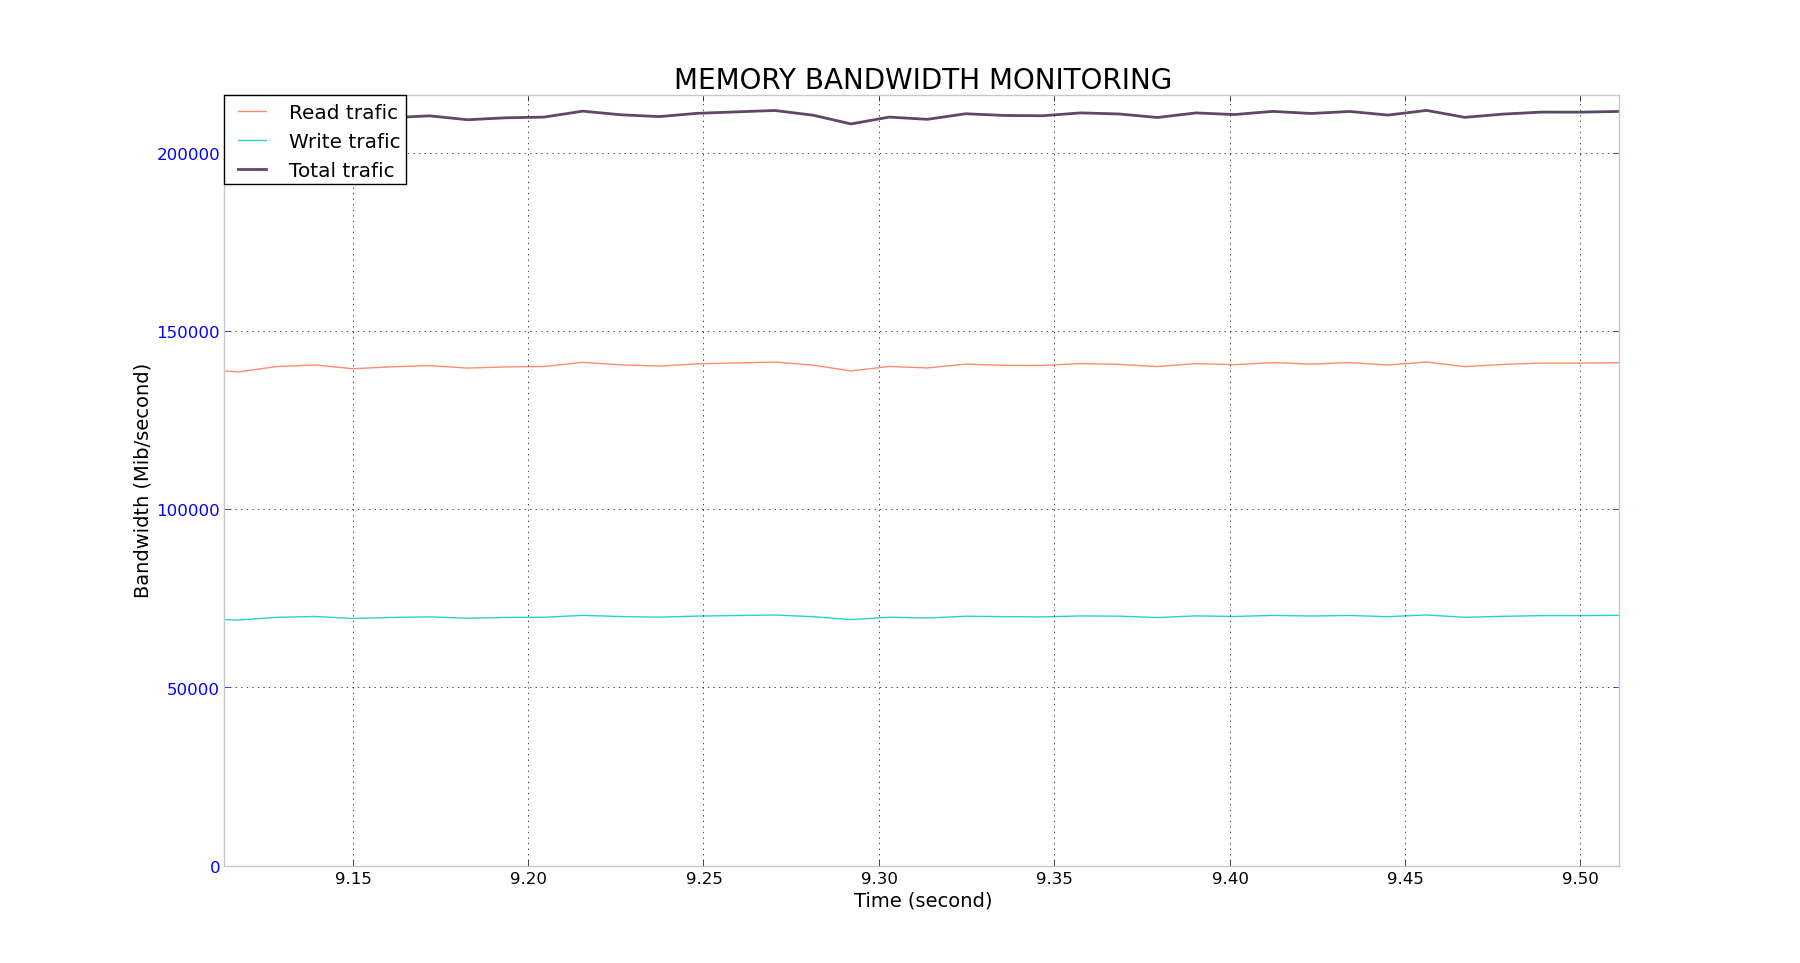
\includegraphics[width=14cm]{images/yamb_stream_triad.png}
        \caption{\label{pic:yamb_stream_triad} Profil de l'utilisation du bus mémoire lors de l'exécution de la fonction \texttt{triad} du benchmark \texttt{STREAM}.}
        \end{figure}


        \paragraph{Autres exemples.} L'outil \verb|YAMB| est utilisé à plusieurs reprises dans ce manuscrit de thèse. Une utilisation est réalisée avec le benchmark \verb=dml_mem= pour caractériser la capacité du cache de dernier niveau à stocker un jeu de données dont la taille s'approche de celle du cache (\autoref{}). Une autre utilisation est présentée dans la \autoref{chap:methodo} pour illustrer l'application de la méthodologie et de l'utilisation des ratios de lecture et écriture pour s'assurer de l'optimalité d'un code.
        
        

    \subsubsection{Mesure de l'impact sur la performance}
    %%%%%%%%%%%%%%%%%%%%%%%%
        Un défaut majeur des outils de mesure de performance est leur impact sur la performance de l'application étudiée. Nous avons réalisé plusieurs tests avec différentes fréquences d'échantillonnage pour estimer l'impact de \verb|YAMB| sur l'application mesurée. Même lorsque la fréquence la plus rapide de \verb=perf= est utilisée (100Hz), l'impact sur la performance est très faible (inférieur à 5\%). Pour une étude suffisamment précise de l'application, obtenir 100 mesures par seconde semble largement suffisant. Nous considérons que cette baisse de performance est suffisamment faible pour s'assurer que la performance mesurée est proche de la performance réelle.
        \newpage
        \section{Profile de l'exécution d'instructions}\label{sec:oprofile}


Cette section présente l'outil \verb=Oprofile++= qui fonctionne en deux étapes: le suivi de performance et l'extraction des noyaux de calculs. Il permet de donner le profile réel des boucles critiques en reliant les évènements mesurés (nombre de cycles et nombre d'instructions exécutées) aux instructions assembleurs associées et de mesurer leur IPC. Il est ensuite possible de quantifier des opportunités d'amélioration, mais aussi de prédire leur performance en fonction d’une amélioration du matériel ou du logiciel.


\begin{lstlisting}[label=lst:dev_op_example, caption=L'outil Oprofile++ permet d'extraire les instructions des noyaux de calculs à partir du code binaire de l'application et d'y associer des mesures d'évènements.]
./oprofile++.sh myapp
    //1\\ START PROFILING
        Starting ... the profiler is now running...
        
    //2\\ EXECUTION 
        Executing ./myapp on CPU #0
        End..
    
    //3\\ STOP PROFILING
    
    //4\\ ANALYSIS 
    cpu_clk_unhalt|       %|  inst_retired|       %|  app_name
               218    50.67            151    26.77   no-vmlinux
               181    42.00            363    64.36   assembly
    
    //5\\ KERNEL EXTRACTION

Kernel from the app name (assembly) 
hot spot with the symbole name (myBench) which takes 64.36% of the profiling
-------------------------------------------------------------------------------
SUM*4       IPC  CYCLES   INSTS   ADDRESS    ASSEMBLY
-------------------------------------------------------------------------------
 1571 |   0.316      38      12    4018f7    vfmadd231pd %zmm0,%zmm1,%zmm2
 1966 |    1.27     594     756    4018fd    vfmadd231pd %zmm0,%zmm1,%zmm3
 1372 |    1.32     503     664    401903    vfmadd231pd %zmm0,%zmm1,%zmm4
  869 |    1.84     436     804    401909    vfmadd231pd %zmm0,%zmm1,%zmm5
  433 |    1.75     433     758    40190f    sub    $0x1,%eax
    0 |       0       0       0    401912    jne    4018f7 <myBench>
-------------------------------------------------------------------------------
LOOP from 401912 to 4018f7 size= 27
    sum(cycles)= 2004 sum(inst)= 2994 #inst= 6 IPC= 1.49 cycles/LOOP= 4.02
-------------------------------------------------------------------------------
\end{lstlisting}

\subsection{Introduction}
%%%%%%%%%%%%%%%%%%%%%%%%%%%%%%%%%%%%%%%%%%%%%%%%%%%%%%%%%%
%%%%%%%%%%%%%%%%%%%%%%%%%%%%%%%%%%%%%%%%%%%%%%%%%%%%%%%%%%
%%%%%%%%%%%%%%%%%%%%%%%%%%%%%%%%%%%%%%%%%%%%%%%%%%%%%%%%%%


    \subsubsection{Motivations}
    %%%%%%%%%%%%%%%%%%%%%%%%%%%%%%%%%%%%%%%%%%%%%%%%%%%%%%%%%%

        
        Pour mener à bien le travail de portage et d'optimisation d’une application, il est important de détecter les \textit{hot spots} et d'identifier les parties du code responsables. Les travaux de Mihail Popov \cite{popov:tel-01412638}  montrent l’importance de les isoler du reste de l’application pour s’y consacrer indépendamment. En effet, les \textit{hot spots} ayant des caractéristiques propres (types d'accès mémoire, pression arithmétique), leur optimisation sera différente. Pour atteindre la performance ultime d’une application, on peut potentiellement porter chaque \textit{hot spot} sur un accélérateur adapté et l’optimiser indépendamment des autres.
        
        De nombreuses applications utilisées dans les systèmes d'informations ne présentent pas ce type de profil et  n'ont pas de goulots d'étranglement évidents. Par conséquent, leurs profils contiennent un grand nombre de fonctions ou de processus dont le temps d'exécution est passé de façon relativement uniforme\cite{Amaral2015}. Ce type de profil est souvent appelé "profil plat" (\textit{flat profil}), car aucune méthode ne domine le temps d'exécution. Dans le calcul haute performance, les \textit{hot spots} sont souvent facilement identifiables, car la majorité du temps d'exécution se déroule dans ces parties du code. 
        
        Le travail d'optimisation d'application est très difficile, notamment sur des applications de calcul haute performance dont le code dépasse souvent les plusieurs milliers de lignes. Il est donc indispensable pour le programmeur d'avoir un outil lui permettant de localiser les \textit{hot spots} de son application.
        

    
    \subsubsection{Objectifs}
    %%%%%%%%%%%%%%%%%%%%%%%%%%%%%%%%%%%%%%%%%%%%%%%%%%%%%%%%%%

        Le programmeur désirant optimiser une application de calcul haute performance doit avoir à sa disposition un outil lui permettant d'obtenir son profil d'exécution détaillant le temps passé dans les différentes parties du code. Une fois ces \textit{hot spots} repérés, l'utilisateur doit connaître précisément comment le code se comporte sur le processeur: type d'instructions utilisées, nombre de cycles par instruction. Utiliser le code source pour cela n'est pas suffisant, car la qualité du code généré par le compilateur peut fortement impacter sa performance (utilisation d'instructions vectorielles). Le second objectif de l'outil proposé doit alors présenter le code assembleur ainsi que les évènements associés pour permettre à l'utilisateur d'identifier la nature du goulot d'étranglement du noyau étudié.
        
        



    \subsubsection{Travaux existants}
    %%%%%%%%%%%%%%%%%%%%%%%%%%%%%%%%%%%%%%%%%%%%%%%%%%%%%%%%%%
        
        De nombreux outils existent pour réaliser l'étude de performance du code, cependant une grande partie ne respecte pas nous pré-requis exprimés en début de chapitre. 
        
        Maqao \cite{Barthou2010} est un outil développé dans le cadre du projet Mont Blanc \cite{Puzovic2012} en source libre.  \verb=MAQAO= permet de détecter les boucles responsables des \textit{hot spots} et d’en analyser leur performance. \verb=MAQAO= comprend le développement de l’outil CQA \cite{Charif-Rubial2014} permettant d’évaluer la qualité du code assembleur et de projeter la performance maximale pour une architecture donnée.  Il est ainsi possible de connaître  les opportunités de vectorisation et des gains potentiels pour les \textit{hot spots} de l'application. Cette analyse nécessite de connaître beaucoup de spécificités de l'architecture utilisée et suppose de que les données soient directement accessibles dans le cache L1. Cet outil est très orienté sur l'analyse de performance de calculs (\textit{FLOP}). Aussi, \verb=MAQAO= permet de réaliser une analyse statique du programme et donne des conseils pour utiliser les drapeaux de compilation adaptés.
        Nous avons eu des difficultés pour l'utiliser: le dépôt \textit{Git} ne permet pas de s'inscrire facilement pour poser des questions, l'absence de page d'informations \textit{wiki} est aussi un manque. L'outil est dépendant de plusieurs librairies qui n'étaient pas disponibles sur les plateformes utilisées. 
        
        Intel propose d'utiliser son compilateur \verb=icc= pour annoter automatiquement les fonctions (\verb=-profile-functions=) ou les boucles (\verb=-profile-loops=) d'une application en instrumentant l'entrée et la sortie de ces parties avec l'instruction \verb=rdtsc=\footnote{\url{https://software.intel.com/en-us/cpp-compiler-developer-guide-and-reference-profile-function-or-loop-execution-time}}. Cette méthode permet d'obtenir une vue d'ensemble de l'utilisation des cycles dans l'application. Il faut cependant posséder le compilateur \verb=icc= et cette méthode n'est compatible qu'avec les plates-formes du constructeur. 
        
        
        \paragraph{Difficultés et verrous.} Le développement d'outil d'analyse de performance est rendu difficile par la faiblesse des compteurs matériels exposée dans la \autoref{sec:edl_hc_conclusion}. Pour assurer un fonctionnement sur une majorité d'architectures, l'outil doit dépendre du minimum possible d'évènements. Il n'est donc pas possible de pouvoir suivre des évènements complexes bien qu'ils puissent être utiles dans l'analyse de performance. La difficulté vient donc de l'impossibilité de développer un outil complet suffisamment portable pour être utilisé sur une majorité d'architectures. 
        

\subsection{Développement}
%%%%%%%%%%%%%%%%%%%%%%%%%%%%%%%%%%%%%%%%%%%%%%%%%%%%%%%%%%
%%%%%%%%%%%%%%%%%%%%%%%%%%%%%%%%%%%%%%%%%%%%%%%%%%%%%%%%%%
%%%%%%%%%%%%%%%%%%%%%%%%%%%%%%%%%%%%%%%%%%%%%%%%%%%%%%%%%%

    L'outil d'analyse de performance de Linux (Oprofile) permet de réaliser un échantillonnage des évènements lors de l'exécution de l'application. Le code source ainsi que le code assembleur peut ensuite être annoté. Cet outil constitue la base du développement de notre version améliorée \verb=Oprofile++=.
    
    \subsubsection{Étape 1: Configuration et activation du profiler}
    %%%%%%%%%%%%%%%%%%%%%%%%%%%%%%%%%%%%%%%%%%%%%%%%%%%%%%%%%%%%%%%%
        
        La première étape qui suit le lancement de l'outil est la collecte d'informations de l'exécution de l'application étudiée. Pour cela, un premier script est utilisé pour activer le \textit{profiler}. Pour faciliter le portage et l'utilisation du profiler sur le plus grand nombre d'architectures nous avons choisi de ne suivre l'évolution que de deux évènements: le nombre de cycles et le nombre d'instructions exécutées. Dans cette première étape, l'outil \verb=Oprofile++= s'occupe de paramétrer le profiler pour compter ces deux évènements à une fréquence qui peut être adaptée pour améliorer la précision de la mesure ou réduire l'impact de l'outil sur les performances de l'application étudiée. 

        Lorsque l'analyse de performance est terminée, un premier fichier est généré contenant les informations de suivie de performance (voir \autoref{lst:dev_op_oprofile_out}). Ce fichier contient pour chaque instruction, son adresse mémoire virtuelle et le nombre d'échantillons mesurés pour les deux évènements. 
        
\begin{lstlisting}[label=lst:dev_op_oprofile_out, caption=Le premier fichier contient les données de performance pour les deux évènements étudiés.]
vma       samples         %    samples         %   app name     symbol name
00402961       20    0.6553         23    0.3100      app_1     matrix_mult
  00402961      6   30.0000          2    8.6957
  00402964      3   15.0000          3   13.0435
\end{lstlisting}   
  
  
        
    \subsubsection{Étape 2: correspondance des évènements et des instructions}
    %%%%%%%%%%%%%%%%%%%%%%%%%%%%%%%%%%%%%%%%%%%%%%%%%%%%%%%%%%%%%%%%%%%%%%%%%%

    La première étape a permis d'obtenir le profile de l'application avec la répartition des deux évènements mesurés. Cependant, aucune information n'est donnée concernant le type des instructions responsables, seule leur adresse mémoire est indiquée. Le but de la deuxième étape est de retrouver l'instruction assembleur correspondante. Pour cela, un deuxième fichier est généré à l'aide de la commande \verb=objdump=. Couplé à l'option \verb=d= cette commande permet de désassembler le binaire de l'application\footnote{objdump - \url{https://linux.die.net/man/1/objdump}}. Dans ce fichier est contenue chaque adresse des instructions de l'application avec l'instruction assembleur correspondante.

\begin{lstlisting}[label=lst:dev_op_obj_out, caption=La commande objdump permet de désassembler le fichier binaire de l'application.]
0000000000401690 <_init>:
  401694:	48 8b 05 5d 29 20 00 	mov    0x20295d(%rip),%rax
\end{lstlisting}  

        Notre première contribution est le développement d'un outil permettant de faire correspondre les adresses mémoires des instructions des deux fichiers. Ainsi, nous possédons dans un même fichier de l'instruction assembleur et des deux compteurs d'évènements associés. 
        

        Les instructions sont regroupées par fonction et les fonctions sont triées par le temps passé à leur exécution. Ce tri en ordre décroissant est très utile lors de l'analyse de performance réalisée par le programmeur, car il commence directement par accéder aux instructions des fonctions les plus longues de l'application. Il est ainsi possible de vérifier que le compilateur a utilisé des instructions vectorielles par exemple. 


    \subsubsection{Étape 3: Extraction des noyaux et analyse de performance}
    %%%%%%%%%%%%%%%%%%%%%%%%%%%%%%%%%%%%%%%%%%%%%%%%%%%%%%%%%%
    
        Les noyaux de calculs (\textit{hot spots}) peuvent se trouver des fonctions différentes du code. Le code assembleur généré peut être très long. Ces deux facteurs rendent l'analyse du programmeur très complexe. Notre deuxième contribution est le développement d'un module permettant d'extraire les noyaux de calculs et de présenter les plus gourmands à l'utilisateur (\autoref{lst:dev_op_extract_out}).
      
\begin{lstlisting}[label=lst:dev_op_extract_out, caption=L'outil Oprofile++ permet de faire correspondre les adresses mémoires des deux fichiers.]
======================================
_FUNCTION_ANALYSIS_ from the app name (assembly) hot spot from the symbole name (myBench) which takes 81.9463% of the profiling
======================================
SUM*4 SUM*3   SUM*2     IPC  CYCLES  INSTS  ADDRESS   ASSEMBLY  
-------------------------------------------------------------------------------
 1657  1221     908 |  2.24     211    472  4201849   vaddsd %xmm0,%xmm1,%xmm2
 1662  1446    1010 |  2.48     697   1731  4201853   vaddsd %xmm0,%xmm1,%xmm3
 1593   965     749 |  3.44     313   1077  4201857   vaddsd %xmm0,%xmm1,%xmm4
 1280  1280     652 |  2.57     436   1122  4201861   vaddsd %xmm0,%xmm1,%xmm5
  844   844     844 |  2.86     216    618  4201865   vaddsd %xmm0,%xmm1,%xmm6
  628   628     628 |  3.14     628   1971  4201869   sub    $0x1,%eax
-------------------------------------------------------------------------------
LOOP from 401d90 to 401d79:
 sum(cycles)= 2501 sum(inst)= 6991 #inst= 7 IPC= 2.79528 cycles/LOOP= 2.50
-------------------------------------------------------------------------------
\end{lstlisting} 

        Les \textit{hot spots} des applications sont souvent caractérisées par la présence de boucles dans le code. Pour extraire ces noyaux de calcul , notre outil recherche les instructions de saut (\textit{jump}) dans le code en parcourant les instructions dans l'ordre du fichier généré lors de l'étape 2. Ainsi, les premiers résultats affichés sont généralement les boucles critiques de l'application. Lorsqu'une boucle est détectée elle est affichée suivie des informations suivantes calculées grâce aux deux compteurs d'évènements: le nombre d'instructions, le nombre de cycles, l'IPC et le nombre de cycles par boucle. 
        
        \paragraph{Sommation d'instruction.} Les processeurs utilisés sont tous superscalaires. Ils sont donc capables d'exécuter plusieurs instructions en un seul cycle. Trouver les instructions exécutées simultanément ainsi que leur nombre n'est pas évident. Pour aider la lecture des résultats, l'outil essaie de sommer le nombre de cycles d'une instruction avec ceux de l'instruction précédente (jusqu'à 4 instructions). Ce calcul permet de mettre en évidence des blocs d'instructions exécutées simultanément comme sur l'\autoref{} de code suivant:
        
        \paragraph{Utilisation recommandée.} La performance d'une application peut sensiblement varier en fonction du jeu de données utilisé. Il est important de réaliser plusieurs profils avec des jeux différents pour isoler les parties du code les plus intéressantes à optimiser. Il est souvent intéressant d'utiliser différents drapeaux de compilation et mesurer leur impact sur le code généré. 
        

\subsection{Résultats}
%%%%%%%%%%%%%%%%%%%%%%%%%%%%%%%%%%%%%%%%%%%%%%%%%%%%%%%%%%
%%%%%%%%%%%%%%%%%%%%%%%%%%%%%%%%%%%%%%%%%%%%%%%%%%%%%%%%%%
%%%%%%%%%%%%%%%%%%%%%%%%%%%%%%%%%%%%%%%%%%%%%%%%%%%%%%%%%%

    Les tests suivant sont réalisés sur un processeur Intel Skylake Gold capable d'exécuter 4 instructions par cycle dont au maximum deux instructions de calculs flottants. Le turbo du processeur est désactivé. 


    \subsubsection{Impact des dépendances}
    %%%%%%%%%%%%%%%%%%%%%%%%%%%%%%%%%%%%%%%%%%%%%%%%%%%%%%%%%%
        La performance de nombreuses applications est détériorée par la présence de dépendances entre les instructions. La seule solution est alors de repenser l'algorithme pour en supprimer le plus possible. Dans cet exemple nous montrons comment la dépendance entre instructions impacte la performance et comment utiliser l'outil \verb=Oprofile++= pour le diagnostiquer. 
        
        L'\autoref{lst:dev_op_dependance} montre le code d'un noyau de calcul généré grâce à l'outil \verb|Kernel Generator| (voir \autoref{sec:kg}). Le noyau consiste en l'exécution de 8 instructions dont chacune utilise comme opérande le résultat de la précédente. À cause de ces dépendances, la performance du noyau est limité par la latence de calcul d'une instruction (4 cycles). La performance maximale atteignable par un tel code est d’une instruction tous les 4 cycles, soit un IPC de 0.25. Ce résultat théorique est bien celui mesuré par notre outil. 
        
        
 \begin{lstlisting}[label=lst:dev_op_dependance, caption=Noyau de calcul présentant une dépendance entre chaque instruction.]
-------------------------------------------------------------------------------
    IPC     CYCLES     INSTS     ADDRESS    ASSEMBLY                         
-------------------------------------------------------------------------------
...
  0.262        825       216      401c27    vfmadd231pd %zmm0,%zmm2,%zmm3
   0.24        800       192      401c2d    vfmadd231pd %zmm0,%zmm3,%zmm4
  0.228        886       202      401c33    vfmadd231pd %zmm0,%zmm4,%zmm5
  0.236        787       186      401c39    vfmadd231pd %zmm0,%zmm5,%zmm6
   0.25        809       202      401c3f    vfmadd231pd %zmm0,%zmm6,%zmm7
  0.271        756       205      401c45    vfmadd231pd %zmm0,%zmm7,%zmm8
  0.232        841       195      401c4b    vfmadd231pd %zmm0,%zmm8,%zmm9
   0.26        759       197      401c51    vfmadd231pd %zmm0,%zmm9,%zmm10
  0.229        808       185      401c57    vfmadd231pd %zmm0,%zmm10,%zmm11
  0.232        772       179      401c5d    vfmadd231pd %zmm0,%zmm11,%zmm12
  0.218        856       187      401c63    vfmadd231pd %zmm0,%zmm12,%zmm13
  0.244        798       195      401c69    vfmadd231pd %zmm0,%zmm13,%zmm14
  0.226        805       182      401c6f    vfmadd231pd %zmm0,%zmm14,%zmm15
  0.244        782       191      401c75    vfmadd231pd %zmm0,%zmm15,%zmm16
  0.254        784       199      401c7b    sub    $0x1,%eax
      0          0         0      401c7e    jne    4018f7 <myBench>
-------------------------------------------------------------------------------
_7_ LOOP from 401c7e to 4018f7 size= 903 
    sum(cycles)= 120060 sum(inst)= 30436 #inst= 152 IPC= 0.254 cycles/LOOP= 600
-------------------------------------------------------------------------------
\end{lstlisting}

        Ce type de dépendance est très courant dans les algorithmes d'application HPC tel que celles réalisant du calcul polynomiales. La solution pour optimiser ce type de noyau est présentée dans la \autoref{sec:kg_out_of_order_dependency}. L'optimisation est réalisée à l'aide du module d'exécution dans le désordre du processeur. Pour en profiter, il est nécessaire de donner suffisamment d'instructions à exécuter à celui-ci. Deux itérations de boucle étant indépendante il est possible de dérouler plusieurs itérations pour calculer plusieurs \textit{streams} à la fois (voir explication dans la \autoref{sec:kg_out_of_order_dependency}). L'\autoref{lst:dev_op_dependance_8_streams} présente le profil de la performance du noyau modifié pour exécuter le calculs de 8 chaînes indépendantes. Appliquer cette optimisation à un code réel peut demander une lourde restructuration du code mais elle est indispensable pour atteindre la performance crête de l'architecture (2 instructions flottantes par cycle).
        

 \begin{lstlisting}[label=lst:dev_op_dependance_8_streams, caption=L'optimisation du noyau précedent permet de présenter au processeur 8 chaînes de calculs indépendantes.]
-------------------------------------------------------------------------------
    IPC     CYCLES     INSTS     ADDRESS    ASSEMBLY                         
-------------------------------------------------------------------------------
...
   2.05        108       221      401c21    vfmadd231pd %zmm0,%zmm9,%zmm2
   1.81         96       174      401c27    vfmadd231pd %zmm0,%zmm10,%zmm3
    2.2        102       224      401c2d    vfmadd231pd %zmm0,%zmm11,%zmm4
   2.56         77       197      401c33    vfmadd231pd %zmm0,%zmm12,%zmm5
   2.32         97       225      401c39    vfmadd231pd %zmm0,%zmm13,%zmm6
   1.89        102       193      401c3f    vfmadd231pd %zmm0,%zmm14,%zmm7
   2.56         86       220      401c45    vfmadd231pd %zmm0,%zmm15,%zmm8
   2.05         92       189      401c4b    vfmadd231pd %zmm0,%zmm16,%zmm9
   2.06         93       192      401c51    vfmadd231pd %zmm0,%zmm2,%zmm10
   2.09         81       169      401c57    vfmadd231pd %zmm0,%zmm3,%zmm11
   1.94        108       210      401c5d    vfmadd231pd %zmm0,%zmm4,%zmm12
   1.92         97       186      401c63    vfmadd231pd %zmm0,%zmm5,%zmm13
   1.97        110       217      401c69    vfmadd231pd %zmm0,%zmm6,%zmm14
   2.61         56       146      401c6f    vfmadd231pd %zmm0,%zmm7,%zmm15
   1.73        117       202      401c75    vfmadd231pd %zmm0,%zmm8,%zmm16
   2.06         94       194      401c7b    sub    $0x1,%eax
      0          0         0      401c7e    jne    4018f7 <myBench>
-------------------------------------------------------------------------------
_7_ LOOP from 401c7e to 4018f7 size= 903 
    sum(cycles)= 15023 sum(inst)= 30413 #inst= 152 IPC= 2.02 cycles/LOOP= 75.1
-------------------------------------------------------------------------------

\end{lstlisting}   




    \subsubsection{Mesure de l'IPC}
    %%%%%%%%%%%%%%%%%%%%%%%%%%%%%%%%%%%%%%%%%%%%%%%%%%%%%%%%%%
    
        L'IPC est une métrique souvent utilisée pour décrire la performance d'une application. L'exemple précédent utilise un noyau artificiel ne comportant que des instructions de calcul. Dans cette seconde expérimentation, nous montrons que conclure de la bonne ou mauvaise performance d'un code à partir de la mesure de l'IPC n'est pas trivial. Le processeur utilisé peut théoriquement exécuter 4 instructions par cycle. Il semble donc évident d'utiliser cette valeur comme la performance maximale à atteindre par l'application. Cependant, il est important de rappeler que si les architectures Skylake peuvent exécuter 4 instructions par cycles, un maximum de deux instructions de calculs flottant peut être exécuté. Pour illustrer nos propos, la performance du noyau présenté dans l'\autoref{lst:dev_op_ipc_missleading} a été mesurée grâce à notre outil \verb=Oprofile++=.

\begin{lstlisting}[label=lst:dev_op_ipc_missleading, caption=Noyau de calcul n'exécutant qu'une opération de calcul par cycle.]
-------------------------------------------------------------------------------
CYCLES       INSTS     ADDRESS    ASSEMBLY                         
-------------------------------------------------------------------------------
  128          145      4018f7    vfmadd231pd %zmm0,%zmm1,%zmm2
  132         1276      4018fd     mov    %bl,%bh
  119          305      4018ff     mov    %cl,%ch
  128          243      401901     mov    %dl,%dh
  105          229      401903    vfmadd231pd %zmm0,%zmm1,%zmm3
  109          189      401909     mov    %bl,%bh
  129         1370      40190b     mov    %cl,%ch
  142          186      40190d     mov    %dl,%dh
  119          256      40190f    vfmadd231pd %zmm0,%zmm1,%zmm4
  135          235      401915     mov    %bl,%bh
  136         1384      401917     mov    %cl,%ch
  138          231      401919     mov    %dl,%dh
  117          199      40191b    vfmadd231pd %zmm0,%zmm1,%zmm5
  117         1109      401921     mov    %bl,%bh
  137          829      401923     mov    %cl,%ch
  127          274      401925     mov    %dl,%dh
  146          303      401927    vfmadd231pd %zmm0,%zmm1,%zmm6
  128          406      40192d     mov    %bl,%bh
  127         1308      40192f     mov    %cl,%ch
  109          222      401931     mov    %dl,%dh
  138          142      401933    vfmadd231pd %zmm0,%zmm1,%zmm7
  119          303      401939     mov    %bl,%bh
  126         1409      40193b     mov    %cl,%ch
  124          209      40193d     mov    %dl,%dh
  123          242      40193f    sub    $0x1,%eax
    0            0      401942    jne    4018f7 <myBench>
-------------------------------------------------------------------------------
_7_ LOOP from 401942 to 4018f7 size= 75 
    sum(cycles)= 3158 sum(inst)= 13004 #inst= 26 IPC= 4.12 cycles/LOOP= 6.31
-------------------------------------------------------------------------------
\end{lstlisting} 
        
        
        Dans cet exemple, nous mesurons l'IPC d'un noyau de calculs dont la performance est de 4.12 instructions par cycle. L'IPC mesurée est supérieur à la performance théorique du processeur car l'instruction de branchement (\verb=jne=) de boucle n'est jamais réellement exécutée grâce au prédicteur de branchement. Contrairement à ce qu'indique cette valeur, la performance du code est très mauvaise car la micro-architecture n'exécute en fait qu'une instruction de calcul par cycle. Le processeur utilise donc la moitié de la performance disponible.
    
        Une architecture exécute toujours un programme donné au maximum de sa capacité. Cependant, la programmation de l'algorithme ainsi que la génération du code peut être de mauvaise qualité. L'outil \verb=Oprofile++= est donc très important pour montrer au programmeur que le code réellement exécuté peut être transformé. L'amélioration des performances d'une application est alors dépendant de la capacité du programmeur à imaginer une autre façon de réaliser ses calculs en utilisant un autre algorithme ou en réordonnant certaines instructions. Dans cette exemple factice, nous pouvons imaginer que la réorganisation des structures de données permettent de supprimer les instructions de déplacement mémoire \verb=mov=. Le code ainsi obtenu est présenté dans  l'\autoref{lst:dev_op_ipc_missleading_ok}. 
    
\begin{lstlisting}[label=lst:dev_op_ipc_missleading_ok, caption=Noyau de calcul exécutant deux opérations de calcul par cycle.]
-------------------------------------------------------------------------------
CYCLES   INSTS     ADDRESS    ASSEMBLY                         
-------------------------------------------------------------------------------
   87      111      4018f7    vfmadd231pd %zmm0,%zmm1,%zmm2
  381      457      4018fd    vfmadd231pd %zmm0,%zmm1,%zmm3
  342      708      401903    vfmadd231pd %zmm0,%zmm1,%zmm4
  403      860      401909    vfmadd231pd %zmm0,%zmm1,%zmm5
  231      694      40190f    vfmadd231pd %zmm0,%zmm1,%zmm6
  335      444      401915    vfmadd231pd %zmm0,%zmm1,%zmm7
  236      725      40191b    sub    $0x1,%eax
    0        0      40191e    jne    4018f7 <myBench>
-------------------------------------------------------------------------------
_7_ LOOP from 40191e to 4018f7 size= 39
    sum(cycles)= 2015 sum(inst)= 3999 #inst= 8 IPC= 1.99 cycles/LOOP= 4.031
-------------------------------------------------------------------------------
\end{lstlisting}

        Après cette transformation, la mesure de l'IPC est alors de 2 instructions par cycle, soit deux fois moins que celui de la version précédente. Pourtant, le noyau exécute bien deux fois plus d'instructions de calculs flottants par cycle. Cette première expérimentation a pour seul objectif d'attirer l'attention de l'utilisateur sur la précaution à prendre pour conclure de la performance d'un code seulement en utilisant la mesure de l'IPC. 
        


    \subsubsection{Impact d'une division ou Kernel de RTM}
    %%%%%%%%%%%%%%%%%%%%%%%%%%%%%%%%%%%%%%%%%%%%%%%%%%%%%%%%%%
    
    \textit{dans cet exemple on peut trouver un exemple d'un code avec une division par une constante qui impacte fortement le code.}\\
    \textit{On montre astuce d'optimisation en remplacant la division pas la mutliplaction de l'inverse}\\
    







\subsection{Conclusion}
%%%%%%%%%%%%%%%%%%%%%%%%%%%%%%%%%%%%%%%%%%%%%%%%%%%%%%%%%%
%%%%%%%%%%%%%%%%%%%%%%%%%%%%%%%%%%%%%%%%%%%%%%%%%%%%%%%%%%
%%%%%%%%%%%%%%%%%%%%%%%%%%%%%%%%%%%%%%%%%%%%%%%%%%%%%%%%%%

    Dans cette section nous proposons un nouvel outil \verb|Oprofile++| qui permet d'extraire les principaux noyaux de calculs d'une application et de donner à l'utilisateur son profil de performance. Contrairement à d'autres outils existants (Vtune, TAU), nous avons voulu développer un outil nécessitant le minimum de dépendances vers des librairies ou des compteurs matériels. Les dépendances et la complexité des outils sont en effet un frein à l'utilisation d'outils plus complexes. En ne dépendant que de deux compteurs présents sur la majorité des architectures et de l'outil de profilage de Linux, nous assurons sa compatibilité avec le plus grand nombre de plateformes. 

    L'augmentation exponentielle de la complexité des architectures et la diversité des applications rend la tâche d'analyse de performance très difficile. Chaque nouvelle configuration (application / architecture) apporte de nouveaux problèmes. Le développement d'un outil réalisant le travail d'analyse de performance automatiquement est ainsi très difficile. Avec \verb|Oprofile++|, nous avons choisi de développer un outil basique, mais qui apporte suffisamment d'informations au programmeur pour qu'il puisse, à l'aide de sa créativité, apporter les modifications nécessaires à l'amélioration du code. L'outil \verb|Opofile++| n'a besoin que du fichier binaire pour pouvoir fonctionner bien que l'accès au code source soit recommandé pour pouvoir appliquer les transformations requises. Si cet outil s'adresse aux programmeurs particulièrement chevronnés, il n'en pas moins un outil essentiel et puissant lorsqu'il est bien utilisé. 
    
    Le profile généré par \verb|Oprofile| permet de localiser les fonctions les modules utilisant le plus de ressources. À partir de ces informations et du profil des évènements enregistrés (nombre de cycle et nombre d'instructions), l'outil \verb|Oprofile++| extrait les noyaux de calculs principaux sur lesquels l'analyse de performance doit se faire. Le profile généré par l'outil permet d'obtenir deux informations essentielles: le type d'instructions exécutées et leur performance. Grâce à cet outil, l'utilisateur peut estimer le gain de performance potentiel d'une optimisation du code. Cette information est essentielle, car les restructurations du code peuvent être difficiles et demander beaucoup d'efforts. Avoir une idée du gain de performance est donc primordial pour motiver la modification du code. 


    \paragraph{Futurs travaux.} L'outil \verb|Oprofile++| peut être difficile à appréhender pour des utilisateurs novices. Nous souhaitons faciliter la lecture du profil des noyaux en apportant d'avantages d'informations à l'utilisateur. Par exemple, nous allons développer une fonctionnalité permettant de calculer la performance maximale théorique du noyau en comptant les instructions de calculs.
    \newpage
        \section{Conclusion}\label{sec:dev_conclusion}
    
    Dans ce chapitre nous présentons les quatre principaux outils développés durant ce travail de thèse. Nous avons commencé par présenter les objectifs à remplir par ces outils et les critères de développement a respecter. Ces critères sont très importants pour assurer leur compatibilité avec le maximum d'architectures, leur facilité d'installation et d'utilisation. 
    Les deux sections suivantes sont consacrées à deux outils permettant la caractérisation des deux parties essentielles de la microarchitecture: le système mémoire et l'unité de calculs d'instruction à nombre flottant. Enfin, les deux dernières sections présentent deux outils permettant de réaliser le suivi de performance: activité du bus mémoire ainsi que l'extraction et la caractérisation des noyaux de calculs d'une application.

%%%%%%%%%%%%%%%%%%%%%%%%%%%%%%%%%%%%%%%%%%%%%
\paragraph{Caractérisation de l'architecture.}
~\\
%%%%%%%%%%%%%%%%%%%%%%%%%%%%%%%%%%%%%%%%%%%%%
    
    La \autoref{sec:dmlmem} présente un premier benchmark appelé \verb|DML_MEM|. Il permet de mesurer la performance soutenable par le système  mémoire pour des accès de type \textit{stride}. Ces accès sont très répandus dans les codes scientifiques utilisant par exemple des algorithmes RTM. Nous avons montré que la complexité des microarchitectures rend impossible la prédiction de performance et que l'utilisation d'un tel benchmark est la seule méthode pour s'assurer de la performance du système mémoire. À travers deux exemples, nous avons vu comment le code source et le compilateur utilisé pouvaient impacter la performance de codes réalisant la même tâche. Nous avons étudié l'impact de la taille des sauts (\textit{strides}), qui pour des raisons architecturales (taille de cache, associativité) peuvent obtenir des performances très inégales. Nous avons remarqué que la totalité des coeurs n'est pas nécessaire pour saturer le bus mémoire et qu'il peut être intéressant d'en désactiver certains pour optimiser la consommation énergétique pour des codes limités par la performance mémoire. Enfin, à travers une série d'exemples nous avons montré comment cet outil pouvait être utilisé et comment sa flexibilité de paramétrage pouvait permettre de réaliser une multitude de tests: fonctionnement des caches, taille des lignes de cache, impact des pages larges, optimisation par déroulement de boucles, performance du préchargement mémoire. Un dernier exemple nous a permis de montrer comment \verb|DML_MEM| pouvait être utilisé pour trouver le couple optimal {fréquence, nombre de coeurs}, permettant de saturer le bus mémoire.\\
    
    Nous avons ensuite présenté l'outil \verb|Kernel Generator| dans la \autoref{sec:kg}. Ce benchmark permet de caractériser la FPU, matériel responsable de l'exécution des instructions de calculs flottants. L'outil utilise des noyaux générés en assembleur pour évaluer très précisément la performance du matériel. Le choix d'utiliser un langage bas niveau permet d'éviter toute intervention du compilateur et nous assure de réaliser des mesures très précises. Grâce aux différentes options, nous avons montré comment utiliser le générateur pour tester différents noyaux de calculs permettant de valider la performance du matériel ou d'en déceler des bogues. Le benchmark peut être utilisé pour réaliser des calculs en simple ou double précision et exécuter des instructions vectorielles de différente taille. Nous montrons comment le générateur de noyaux a été utilisé pour mesurer l'impact de la taille des instructions vectorielles et de l'utilisation du \textit{turbo} sur la fréquence du processeur. Dans un second exemple, nous avons montré comment une caractéristique majeure des architectures Haswell pouvait être détectée facilement. Grâce à une option, nous avons enfin présenté comment l'outil pouvait mesurer la performance du système d'exécution dans le désordre et évaluer le nombre de \textit{stream} de calculs indépendant qu'il parvenait à exécuter. Cette information est une caractéristique majeure pour les applications utilisant plusieurs chaînes de calculs indépendantes.  
    
    
%%%%%%%%%%%%%%%%%%%%%%%%%%%%%%%%%%%%%%%%%%%%%
\paragraph{Suivi et analyse de performances.}
~\\
%%%%%%%%%%%%%%%%%%%%%%%%%%%%%%%%%%%%%%%%%%%%%
    
    Dans la \autoref{sec:yamb} nous présentons un premier outil essentiel pour l'analyse de performance. Appelé \verb=YAMB=, il permet de réaliser le suivi de l'activité du bus mémoire en mesurant le nombre transaction en lecture et en écriture actuellement réalisées sur le bus ainsi que le nombre de \textit{miss} dans le dernier niveau de cache. Séparer le trafic en lecture et en écriture est une fonctionnalité essentielle de l'outil. Nous montrerons comment utiliser ce ratio dans le chapitre suivant. Pour faciliter l'analyse du code, une bibliothèque a été développée permettant depuis le code source d'annoter les parties du code étudiées.\verb=YAMB= est basé sur \verb=perf=, l'outil de suivi de performance de Linux. En utilisant le sous-système de performance \verb=Perf Events=, nous assurons le maximum de compatibilité entre différentes plateformes. Enfin, nous avons étudié l'impact de l'utilisation de l'outil sur les performances de l'application étudiée. La baisse de performance mesurée sur un benchmark tel que \verb=STREAM= est inférieur à 5\%.\\
    
    Enfin, dans la \autoref{sec:oprofile}, nous présentons un nouvel outil d'analyse de performance nommé \verb=Oprofile++=. Cet outil permet d'extraire les boucles critiques d'une application (les \textit{hot spots}) et d'extraire leur profile de performance. Grâce à cet outil, une analyse bas niveau peut être réalisée et permettre d'obtenir des pistes pour l'optimisation des codes. Dans cette section, nous discutons aussi l'utilisation de l'IPC pour caractériser la performance d'un code. Pour terminer, nous avons étudié plusieurs exemples concrets d'analyse de code et montré comment l'outil pouvait être utilisé.
    
    
%%%%%%%%%%%%%%%%%%%%%%%%%%%%%%%%%%%%%%%%%%%%%
\paragraph{Conclusion.}
~\\
%%%%%%%%%%%%%%%%%%%%%%%%%%%%%%%%%%%%%%%%%%%%%
    
    Dans ce chapitre, nous avons présenté quatre outils permettant de réaliser la caractérisation d'une architecture ainsi que le suivi de la performance d'une application. Ces quatre outils ont été élaborés pour respecter les critères de développement présenté dans la première section. 
    
    L'analyse de performance est un travail difficile, nécessitant de nombreuses connaissances du comportement des architectures. Pour aider le développeur dans ce travail, nous proposons quatre nouveaux outils. Chacun d'entre eux permet de répondre à un nombre limité de questions. Contrairement à des solutions existantes comme \verb|VTune|, nous avons choisi de développer plusieurs outils indépendants répondant chacun à une question précise. Cette approche permet une plus grande flexibilité pour l'utilisateur. Nous avons vu à travers divers exemples, que malgré la simplicité apparente des outils, de nombreuses caractéristiques peuvent être établies. Nous espérons qu'en réduisant la complexité de l'outillage, l'adoption des outils auprès des programmeurs sera plus grande.
    
    Les outils présentés dans ce chapitre permettent d'obtenir certaines informations sur l'architecture ou sur la performance d'une application. Cependant, leur réelle efficacité réside dans la faculté de l'utilisateur à les utiliser ensemble pour mener son travail d'analyse. Dans le chapitre suivant, nous verrons comment ces outils utilisés avec la bonne méthodologie peuvent permettre de mener une analyse très fine des codes de calculs haute performance.
    \else
        \section{Monitoring du bus mémoire}\label{sec:yamb}


Cette section présente l'outil YAMB (\textit{Yet Another Memory Bandwidth profiling tool}). YAMB établit le profil de chaque contrôleur de mémoire en mesurant le nombre de transactions (lecture et écriture) ainsi que le nombre d'évènements \textit{miss} dans le dernier niveau de cache (LLC). Ensuite, il utilise un script python pour dessiner un graphique montrant l'évolution des trois métriques.

\begin{figure}[h!]
\center
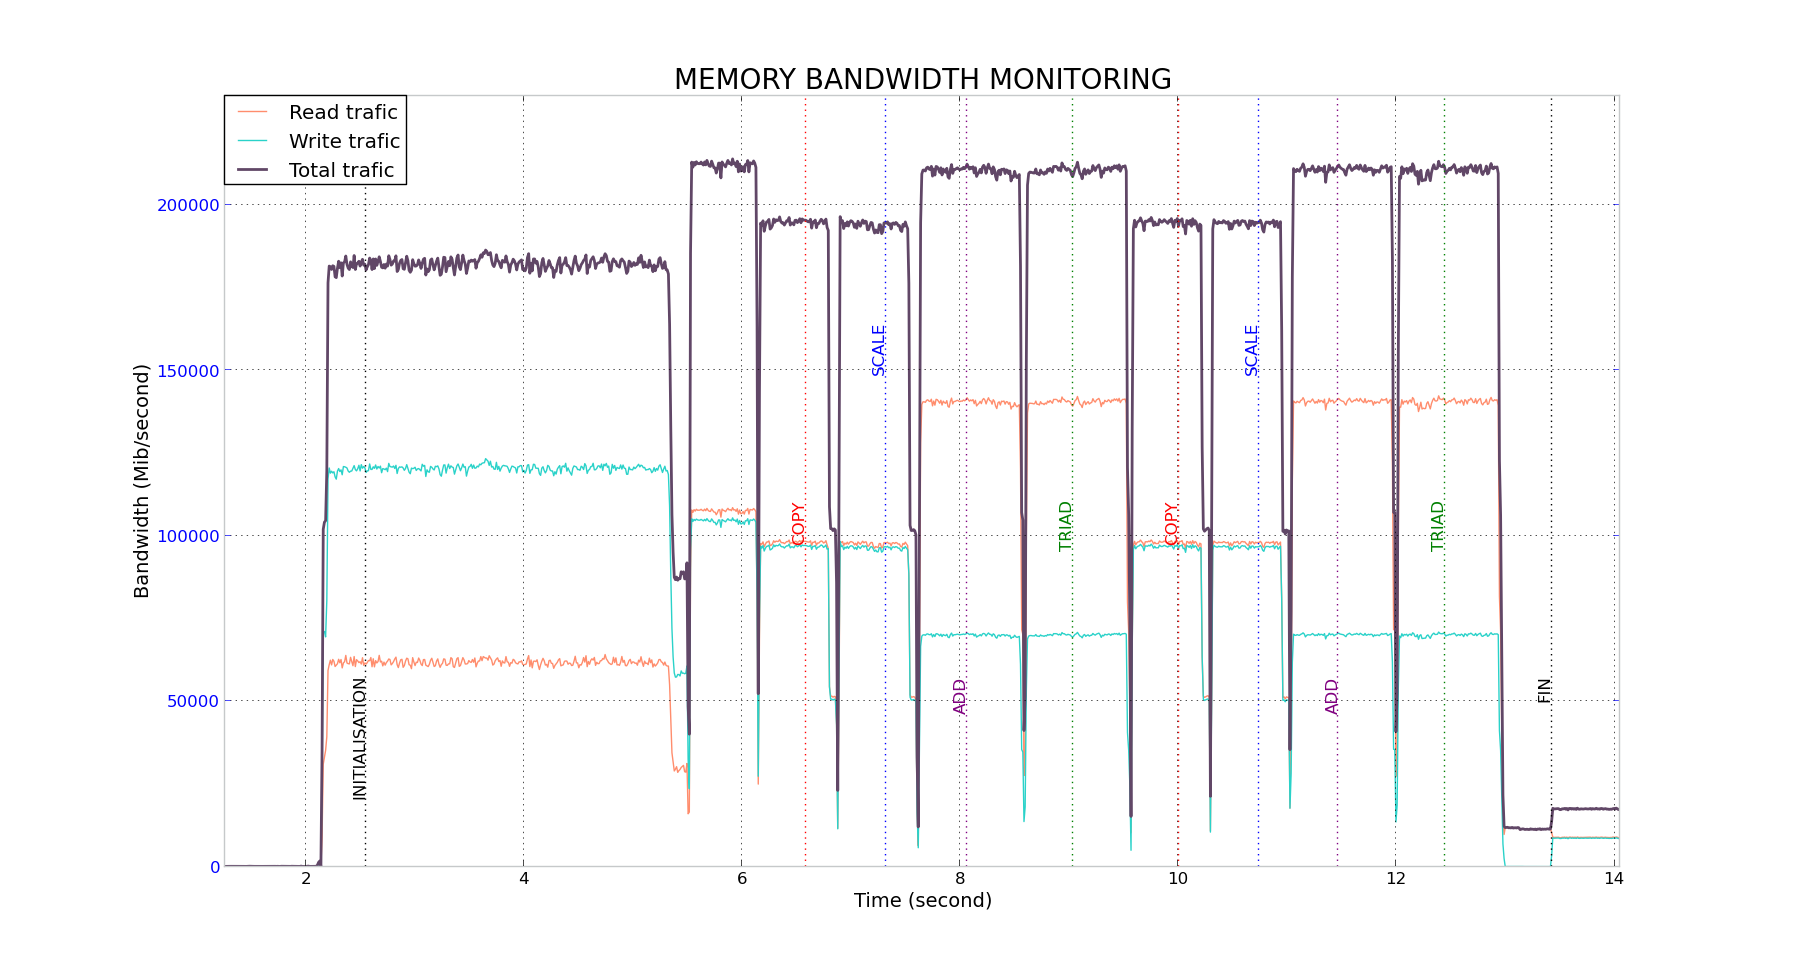
\includegraphics[width=16cm]{images/yamb_stream.png}
\caption{\label{pic:yamb_stream} Exemples d'utilisation de l'outil \texttt{YAMB} pour suivre l'activité du bus mémoire lors de l'exécution du benchmark \texttt{STREAM} pour deux itérations des 4 noyaux de calculs: \texttt{copy}, \texttt{scale}, \texttt{add} et \texttt{triadd}.}
\end{figure}




\subsection{Introduction}
%%%%%%%%%%%%%%%%%%%%%%%%%%%%%%%%%%

    \subsubsection{Motivation}
     %%%%%%%%%%%
     
        Comme présenté dans le \autoref{chap:sota:materiel}, le bus mémoire d'une architecture Von Neuman est le principal goulot d'étranglement des performances des applications de calculs intensifs\cite{Drepper2007}. Le bus mémoire est une ressource partagée par les coeurs d'un même processeur. La mauvaise utilisation de celui-ci par un coeur affecte la performance des autres. Nous observons une augmentation du nombre de coeurs sur les processeurs de dernière génération sans réelle évolution de la performance du bus mémoire. Cette disparité résulte en une augmentation d'accès concurrents à cette ressource partagée limitant la performance des applications. Il est donc primordial de s'assurer de son utilisation optimale (saturation et transferts de données utiles). Pour s'en assurer, il n'est pas possible de réaliser une mesure sur la totalité de l'application (ou d'un noyau de calculs). En effet, une application peut être limitée par la performance du bus, sans qu'il soit saturé. En effet, le déclenchement des accès mémoire par le processeur n’est pas toujours optimal pour saturer le bus mémoire sur la totalité de l'exécution. Par exemple si les accès sont tous réalisés au même moment, le bus peut être saturé pendant un court instant et être ensuite inutilisé. Sur la totalité de l'exécution, on obtiendra une mesure qui indiquera que le bus n'est pas saturé alors qu'il s'agit bien du goulot d'étranglement des performances de l'application. Le bus mémoire étant une ressource critique, il doit être utilisé pour transférer le plus possible de données utiles. Les transferts entre la mémoire et le processeur se font  par paquet (ligne de cache). Il est primordial que le maximum des données présent dans cette ligne de cache soit utilisées pour un calcul lorsque celle-ci est transférée vers le processeur. Pour cela, une adaptation des structures de données peut être nécessaire.
    
    \subsubsection{Objectifs}
    %%%%%%%%%%%
    
        L'objectif de l'outil présenté dans cette section est de répondre aux deux prérogatives indiquées dans précédemment: saturation du bus et utilisation effective. Pour y répondre, l'utilisateur doit posséder un outil lui permettant de suivre son activité avec une résolution fine (de l'ordre de la milliseconde). L'outil en question doit pouvoir distinguer les accès réalisés en lecture et en écriture pour pouvoir s'assurer de l'utilisation effective du bus. Cette méthodologie est présentée dans la section \autoref{sec:smm}.

    \subsubsection{Verrous}
    %%%%%%%%%%%
        
        
        Le système d'exploitation n'a généralement pas connaissance de l'évolution des accès mémoire, contrairement à d'autres ressources comme les I/O où le système d'exploitation réalise l'intermédiaire avec l'application. Mis à part certaines tâches comme la gestion des pages, les accès mémoire sont réalisés par le contrôleur mémoire. Comme étudié dans la \autoref{sec:edl_perf_uncore}, ces compteurs sont situés sur les PMU \textit{uncore}. Sur des architectures modernes telles que les processeurs Intel Skylake, ces compteurs comptent précisément tous les accès mémoire réalisés en distinguant la lecture et  l'écriture. Cependant, comme les compteurs ne sont associés à aucun coeur, il est impossible de faire correspondre un accès mémoire au coeur et donc au processus qui en est responsable. Notre outil a pour objectif d'analyser l'activité d'applications HPC qui utilisent généralement tous les coeurs des processeurs pour la même application. Cette particularité n'est donc pas un verrou majeur pour notre développement. Pour des outils nécessitant plus de précision \cite{Larysch2016}, l'utilisation de ces compteurs n'est cependant pas possible. Les moyens disponibles pour les programmer sont complexes et propres à chaque architecture. Le développement d'un outil utilisant une programmation directe des compteurs rend très difficile la portabilité de l'outil sur différentes architectures.
  
          
    \subsubsection{État de l'art}
    %%%%%%%%%%%%%%%%%%%%%%%%%%%%%%%
    
        Les évènements se produisant sur un processeur peuvent être comptés à l'aide de compteurs matériels. Ils sont accessibles par le biais de composants appelés Performance Monitor Units (PMU). Sur les CPU modernes, il y a au moins deux PMU : une sur le noyau et une sur le socket responsable des évènements qui s'y rapportent (comme l'accès mémoire). Ces compteurs varient d'une architecture à l'autre, ou d'un modèle de processeur à l'autre, ce qui les rend difficiles à programmer et à maintenir. Que ce soit pour le core ou le uncore, ces méthodes sont assez complexes à utiliser et à maintenir. C'est pourquoi nous utilisons des interfaces de haut niveau telles que \textit{PAPI} ou \textit{perf} qui nous permettent de ne plus dépendre de l'implémentation des compteurs à bas niveau. 
        
        De nombreux outils ont été développés pour suivre l'activité du CPU (voir \autoref{sec:edl_monitoring_tools}). Intel propose deux outils, \verb|VTune|\cite{reinders2005vtune} et Intel MBM \footnote{Intel MBM - \url{https://github.com/intel/intel-cmt-cat/wiki}}. Le premier est un outil propriétaire nécessitant une licence payante. Le deuxième est proposé en libre accès sur le dépôt en ligne d'Intel mais n'est compatible qu'avec des architectures Intel.
        
        D'autres outils tels que \verb=TAU= ou \verb=Extrae= présentent de nombreuses informations à l'utilisateur qui rendent difficile la compréhension des résultats. De plus, ce grand nombre d'informations nécessite généralement l'utilisation de plusieurs compteurs matériels qui peuvent ne plus être présents d'une architecture à l'autre. La complexité des outils peut aussi les rendre dépendants de librairies externes non compatibles avec certaines architectures rendant leur utilisation impossible (\verb|MAQAO|).
        
        L'outil \textit{Likwid} propose de mesurer les données transférées (GB) et leur débit (GB/s) pour un noyau de calcul. Il peut aussi générer des traces pour suivre plus précisément l'utilisation du bus mémoire, mais l'outil de visualisation des données n'est plus supporté.
        
        D'autres travaux tels que \textit{Memguard}\cite{Yun2013} mesurent le nombre de \textit{miss} dans le dernier niveau de cache pour en déduire le trafic du bus mémoire. Malheureusement, avec la complexification des architectures et l'utilisation constante des unités de préchargement mémoire, certains transferts mémoires sont réalisés avant qu'un évènement \textit{miss} ne soit déclenché. Il n'est donc plus possible de mesurer le trafic mémoire avec ces techniques-là. 

      
    

\subsection{Développement}
%%%%%%%%%%%%%%%%%%%%%%%%%%%%%%%%%%

    \subsubsection{Choix de l'interface}
        
            De nombreux outils et interfaces ont été développés pour accéder aux compteurs matériels avec leurs avantages et leurs inconvénients. Les principales contraintes de nos développements sont la portabilité des outils et l'accès libre aux sources. Likwid et \textit{Perf Events} sont les outils répondant au maximum des critères de développement énoncés précédemment. Cependant, l'outil de visualisation de Likwid n'est plus supporté. Pour ces raisons et afin d'éviter une surcouche supplémentaire, nous avons choisi de développer nos outils en nous basant sur le système de suivi de performance \textit{Perf Events}. En effet, son intégration dans le noyau lui assure une certaine pérennité et il permet d'utiliser des évènements natifs lorsque les noms symboliques ne sont pas supportés. Ainsi, nous nous assurons un maximum de compatibilité avec les architectures émergentes.
            
            Bien qu'il s'agisse avant tout d'un outil d'espace utilisateur, la commande perf fait partie du noyau Linux du point de vue du développement. Faire partie de Linux assure une haute exigence du développement du code ainsi qu'un support au fil des versions du noyau. Lorsque le noyau supporte le nom symbolique des évènements, \textit{perf} est très simple à utiliser. Dans le cas contraire, \textit{Perf Events} offre la possibilité aux utilisateurs expérimentés d'encoder leurs propres évènements.
            
            L'inclusion de \textit{Perf Events} au projet Linux peut aussi être un inconvénient en rendant l'outil intrinsèquement lié à la version du noyau Linux. Ceci implique que pour utiliser les nouvelles fonctionnalités de perf il faut généralement installer la version du noyau correspondante. La deuxième difficulté vient de l'appel système \textit{perf\_event\_open}. S'il permet d'éviter à l'utilisateur d'écrire manuellement les différents bits de configuration des MSR, beaucoup de travail reste à faire pour le développeur désireux de profiler ses applications. Parce que Linux supporte de nombreux processeurs différents possédant différentes versions de PMU, les développeurs de noyau ont dû laisser la charge de beaucoup de détails de microarchitecture de bas niveau dépendant du code utilisateur. En conséquence, cet appel système est très complexe à utiliser et ne peut pas être utilisé de manière portable. Les principales difficultés consistent à trouver les événements à compter ou à échantillonner, à configurer tous les paramètres à transmettre à l'appel système et à effectuer plusieurs appels système en fonction du nombre de \textit{threads} de l'application profilée et du nombre de coeurs utilisés. Ces différentes difficultés (programmation, portabilité) ont été les principales motivations du développement d'autres outils tels que PAPI, Intel Performance Counter Monitor (PCM) ou NUMAP\cite{Selva2017}.

    \subsubsection{Perf Events}
    %%%%%%%%%%%%%%%%%%%%%%%%
     
        YAMB est plus un utilitaire pour la commande \textit{perf} qu'un outil autonome. Comme présenté dans \autoref{sec:edl_profiling_perf}, \textit{perf} est l'outil de profilage de Linux, et nous espérons que sa large disponibilité le rendra facilement utilisable par le plus grand nombre de personnes.  En raison des permissions limitées que les utilisateurs ont sur les clusters l'outil doit utiliser une interface ne nécessitant pas de droits privilégiés (\textit{root}) pour y accéder. Du fait du développement de l'interface \verb=perf_event= dans le code noyau il est possible pour l'administrateur d'autoriser les utilisateurs normaux à accéder aux compteurs. Cela peut être fait en écrivant la valeur 1 dans le fichier \verb=/proc/sys/kernel/perf_event_paranoid=.
        
        La commande \verb=perf= peut être utilisée pour programmer les PMU \textit{uncore} et accéder aux compteurs des contrôleurs mémoires. L'outil YAMB utilise cette commande pour configurer les PMU pour qu'elles comptent les transactions en cours sur chaque canal mémoire, en lecture et en écriture. La commande peut aussi être utilisée pour compter le nombre d'évènements \textit{miss} dans le cache de dernier niveau (optionnel).
        
        Le coeur de l'outil de profilage YAMB est le lancement de la commande \verb=perf= en arrière-plan et le traitement des données dans un fichier de sortie. Ensuite, un script peut être utilisé pour dessiner le graphique. 
        L'outil \verb=YAMB= reçoit deux options \verb=--start= et \verb=--stop=. L'utilisation de la première option lance la commande \verb|perf| avec les arguments adéquats en arrière-plan. L'appel du script avec l'option \verb=--stop= s'occupe de retrouver le \verb|PID| du processus de \verb|perf| pour l'arrêter et de sauver les données collectées dans un fichier. Entre ces deux appels, l'utilisateur peut exécuter son application ou attendre un certain temps:
\begin{lstlisting}[language=bash]
$ ./yamb.sh --start
$ ... sleep | run application ...
$ ./yamb.sh --stop
\end{lstlisting}
        Comme le montre l'extrait de code ci-dessus, l'avantage de cet outil réside dans la flexibilité de son utilisation. Il est courant dans le travail d'analyste de vouloir suivre l'exécution d'une application pendant une période donnée. L'exécution pouvant durer plusieurs heures, il est important que notre outil ne nécessite pas d'attendre l'exécution complète de l'application pour prodiguer ses résultats. Grâce à cette approche, l'utilisateur se connecte à un serveur durant l'exécution de l'application, lance le profiler pendant une période voulue et l'arrête pour analyser les résultats. Cette méthodologie permet de laisser l'application s'exécuter. Le code de l'application pouvant être instrumenté pour annoter le graphique de résultat, il est possible de tracer et d'identifier les parties du programme mesurée par l'outil.n.
        

    \subsubsection{Annotation}
    %%%%%%%%%%%%%%%%%%%%%%%%

        Pour aider à identifier la zone de code responsable du trafic mémoire, une librairie a été développée. Elle permet d'annoter le code d'une application (\verb=c= et \verb=fortran=) à l'aide d'un \verb=label= et d'une \verb=couleur=. La librairie ne contient que la fonction \verb=yamb_annotate_set_event= permettant d'écrire ces informations en plus d'un pas de temps dans un fichier de journal:
\begin{lstlisting}[label=lst:yamb_api ,language=C]
int yamb_annotate_set_event(const char * label, const char *couleur){
...
    m_LOG_FILE << time_step << " " << label << " " << couleur << endl;
...
}
\end{lstlisting}
    


\subsection{Résultats}
%%%%%%%%%%%%%%%%%%%%%%%%%%%%%%%%%%


    \subsubsection{Application à STREAM}
    %%%%%%%%%%%%%%%%%%%%%%%%

        Cette section présente un exemple d'utilisation de \verb=YAMB= appliqué au benchmark \verb=STREAM=. Pour mieux comprendre l'évolution du trafic mémoire, la première étape est d'annoter les différentes parties du codes intéressantes. Pour cela, nous utilisons la fonction \verb=yamb_annotate_set_event= pour ajouter une trace sur le graphique lors de chaque début de benchmark. L'analyse peut ensuite être lancée avec les commandes suivantes:
    
\begin{lstlisting}[label=lst:yamb_api ,language=C]
$ ./yamb.sh --output log_stream --command ./stream.SKL.192GB
$ python ./format_log.py --data log_stream.perf.mem --annotate log_stream.annotate
\end{lstlisting}

        Le résultat de cette première expérimentation peut être vu sur la \autoref{pic:yamb_stream}. L'utilisation du graphique peut ensuite permettre d'agrandir les parties plus intéressantes comme le noyau de calcul \verb=triad=(voir \autoref{pic:yamb_stream_triad}). Grâce à la distinction entre les accès mémoire réalisés en lecture ou en écriture, nous pouvons remarquer que le ratio de transfert est de deux lectures pour une écriture.
        
        
        \begin{figure}
        \center
        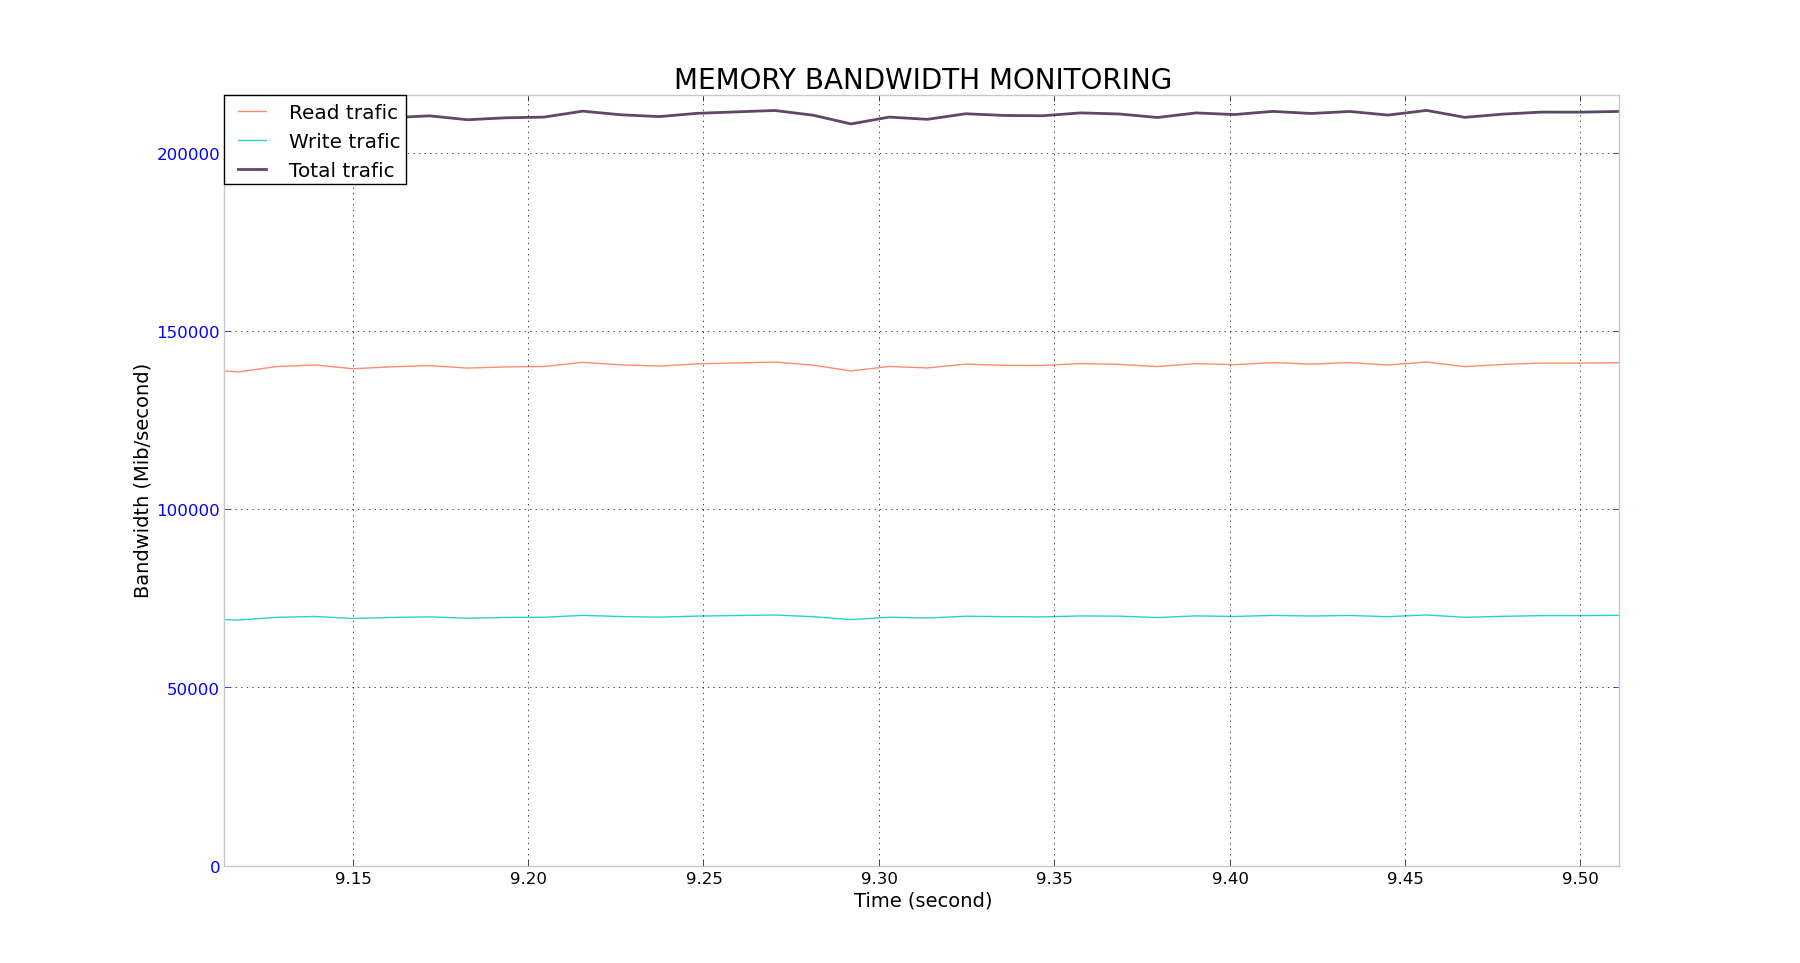
\includegraphics[width=14cm]{images/yamb_stream_triad.png}
        \caption{\label{pic:yamb_stream_triad} Profil de l'utilisation du bus mémoire lors de l'exécution de la fonction \texttt{triad} du benchmark \texttt{STREAM}.}
        \end{figure}


        \paragraph{Autres exemples.} L'outil \verb|YAMB| est utilisé à plusieurs reprises dans ce manuscrit de thèse. Une utilisation est réalisée avec le benchmark \verb=dml_mem= pour caractériser la capacité du cache de dernier niveau à stocker un jeu de données dont la taille s'approche de celle du cache (\autoref{}). Une autre utilisation est présentée dans la \autoref{chap:methodo} pour illustrer l'application de la méthodologie et de l'utilisation des ratios de lecture et écriture pour s'assurer de l'optimalité d'un code.
        
        

    \subsubsection{Mesure de l'impact sur la performance}
    %%%%%%%%%%%%%%%%%%%%%%%%
        Un défaut majeur des outils de mesure de performance est leur impact sur la performance de l'application étudiée. Nous avons réalisé plusieurs tests avec différentes fréquences d'échantillonnage pour estimer l'impact de \verb|YAMB| sur l'application mesurée. Même lorsque la fréquence la plus rapide de \verb=perf= est utilisée (100Hz), l'impact sur la performance est très faible (inférieur à 5\%). Pour une étude suffisamment précise de l'application, obtenir 100 mesures par seconde semble largement suffisant. Nous considérons que cette baisse de performance est suffisamment faible pour s'assurer que la performance mesurée est proche de la performance réelle.
        \newpage
    \fi 
%\printbibliography[heading=references,segment=\therefsegment]
   